\documentclass[amsmath,amssymb,superscriptaddress]{revtex4-1}
\usepackage[latin1]{inputenc}
\usepackage{amsfonts}
\usepackage{amssymb}
\usepackage{float}
\usepackage{graphicx}
\usepackage{hyperref}
\usepackage[detect-all]{siunitx}
\usepackage{xr}
\externaldocument{paper}
\usepackage{rotating}
\usepackage[margin=2cm]{geometry}
\renewcommand{\thefigure}{S\arabic{figure}}
\renewcommand{\theequation}{S\arabic{equation}}
\renewcommand{\thesection}{S\arabic{section}}
\renewcommand{\thetable}{S\Roman{table}}

\begin{document}
\title{SI for ``Bayesian determination of the effect of a deep eutectic solvent on the
structure of lipid monolayers''}% Force line breaks with \\%
\author{A.~R.~McCluskey}
\thanks{A.R.M. and A.S.-F. contributed equally to this work}
\email{a.r.mccluskey@bath.ac.uk/andrew.mccluskey@diamond.ac.uk}
\affiliation{Department of Chemistry, University of Bath, Claverton Down,
Bath, BA2 7AY, UK}
\affiliation{Diamond Light Source, Harwell Campus, Didcot, OX11 0DE, UK}

\author{A.~Sanchez-Fernandez}
\thanks{A.R.M. and A.S.-F. contributed equally to this work}
\altaffiliation[Present address: ]{Department of Food Technology, Lund
University, SE-211 00 Lund, Sweden.}
\affiliation{Department of Chemistry, University of Bath, Claverton Down,
Bath, BA2 7AY, UK}
\affiliation{European Spallation Source, SE-211 00 Lund, Sweden}

\author{K.~J.~Edler}
\affiliation{Department of Chemistry, University of Bath, Claverton Down,
Bath, BA2 7AY, UK}

\author{S.~C.~Parker}
\affiliation{Department of Chemistry, University of Bath, Claverton Down,
Bath, BA2 7AY, UK}

\author{A.~J.~Jackson}
\affiliation{European Spallation Source, SE-211 00 Lund, Sweden}
\affiliation{Department of Physical Chemistry, Lund University, SE-211 00
Lund, Sweden}

\author{R.~A.~Campbell}
\affiliation{Division of Pharmacy and Optometry, University of Manchester,
Manchester, UK}
\affiliation{Institut Laue-Langevin, 71 avenue des Martyrs, 38000, Grenoble,
France}

\author{T.~Arnold}
\email{tom.arnold@esss.se}
\affiliation{Department of Chemistry, University of Bath, Claverton Down,
Bath, BA2 7AY, UK}
\affiliation{Diamond Light Source, Harwell Campus, Didcot, OX11 0DE, UK}
\affiliation{European Spallation Source, SE-211 00 Lund, Sweden}
\affiliation{ISIS Neutron and Muon Source, Science and Technology Facilities
Council, Rutherford Appleton Laboratory, Harwell Oxford, Didcot, OX11 0QX,
UK}

\date{\today}

\maketitle

All datasets, figure file and analysis/plotting scripts, allowing for a fully reproducible analysis of all work presented herein. See DOI: 10.5281/zenodo.2538002

\section{XRR parameters at each surface pressure}
Tables \ref{tab:liptab1}-\ref{tab:liptab4} give the best fit values for the custom model that were fitted to each surface pressure, for each lipid. These values were used for comparison to assess the effect of the choline chloride:glycerol on the lipid.

\section{Neutron reflectometry and SLD profiles}
Figure \ref{fig:neutron} shows the neutron reflectomery and scattering length density profiles for DMPC at \SI{25}{\milli\newton\per\meter} (two contrasts) and DPPC at \SI{15}{\milli\newton\per\meter} (two contrasts).

\section{Grazing incident X-ray diffraction (GIXD)}
\label{sec:gixd}
We have already indicated that the surface pressure was measured using an Aluminium Wilhelmy plate because the standard paper plates did not wet properly. This method did allow us to measure Langmuir isotherms, but these were inconsistent and as such, not a reliable method for determining the phase of the lipid monolayers.
Instead we were able to measure GIXD for DPPC and DMPC over a range of different surface pressures and temperatures and representative data from these measurements are shown in Figure \ref{fig:gixd} for \SI{30}{\milli\newton\per\meter} and \SI{22}{\celsius} (and \SI{7}{\celsius} for DMPC).
Unfortunately, despite our best efforts, the quality of GIXD data obtained was not entirely satisfactory.
All of data contains a weak artefact which we believe is due to scattering from the Teflon trough, which is probably due to the relatively low meniscus of the DES (due to its low surface tension compared to water). In addition we cannot see the expected (1,1) peak observed for these lipids on water.
It is unclear whether this is because these peaks are absent or too weak to be measured.
Nonetheless, Figure \ref{fig:gixd} shows clear diffraction peaks (which we assume to be the (2, 0)) for DPPC at \SI{22}{\celsius} and for DMPC at \SI{7}{\celsius}.
These peaks are also visible at lower surface pressures (data not shown).
The presence of any diffraction feature indicates the presence of an LC phase at these temperatures.
Importantly there is no such peak observed for DMPC at \SI{22}{\celsius} (see \ref{fig:gixd}), indicating that DMPC is in the LE phase at this temperature.
The position of the (2,0) peak, approx \SI{1.48}{\per\angstrom}, is similar to that found under the same conditions in water.\cite{Watkins2009}
We therefore assume that the phase behaviour on the DES is similar to that observed on water and that the phases observed at \SI{30}{\milli\newton\per\meter} are the same at the other surface pressures measured with XRR and NR.
While we have no direct evidence, we have extended this assumption to DLPC and DMPG since there is no reason to believe that the phases of these molecules should be different from that observed for DMPC.

\section{Probability distribution functions}
The two-dimensional probability distribution functions (PDFs) for all parameters and all lipids from the X-ray reflectometry models are given in Figures \ref{fig:dlpc1}-\ref{fig:dmpg4}.
The two-dimensional probability distribution functions (PDFs) for all parameters and all lipids from the neutron reflectometry models are given in Figures \ref{fig:dmpcn1}-\ref{fig:dppcn2}.

\section{Tables and Figures}

%
\begin{table}
  \centering
	\caption{\ The best-fit values, and associated 95 \% confidence intervals for the varying parameters in the XRR models, at the highest surface pressure (SP) measured. The values for $\phi_h$ were obtained from the use of Eqn. \ref{equ:phih}}
	\label{tab:liptab1}
	\begin{tabular}{l|l|l|l|l}
		Lipid & DLPC & DMPC & DPPC & DMPG \\
    SP/mNm$^{-1}$ & 30 & 30 & 25 & 25 \\
		\hline
		$\sigma_{t,h,s}$/\AA & \input{../output/dlpc/rough35.txt} & \input{../output/dmpc/rough40.txt} & \input{../output/dppc/rough30.txt} & \input{../output/dmpg/rough30.txt} \\
    $d_t$/\AA & \input{../output/dlpc/tail35.txt} & \input{../output/dmpc/tail40.txt} & \input{../output/dppc/tail30.txt} & \input{../output/dmpg/tail30.txt} \\
    \hline
    $V_t$/\AA$^3$ & \input{../output/dlpc/vt.txt} & \input{../output/dmpc/vt.txt} & \input{../output/dppc/vt.txt} & \input{../output/dmpg/vt.txt} \\
		$V_h$/\AA$^3$ & \input{../output/dlpc/vh.txt} & \input{../output/dmpc/vh.txt} & \input{../output/dppc/vh.txt} & \input{../output/dmpg/vh.txt} \\
		$d_h$/\AA & \input{../output/dlpc/head.txt} & \input{../output/dmpc/head.txt} & \input{../output/dppc/head.txt} & \input{../output/dmpg/head.txt} \\
    \hline
    $\phi_h$/$\times10^{-2}$ & \input{../output/dlpc/solh35.txt} & \input{../output/dmpc/solh40.txt} & \input{../output/dppc/solh30.txt} & \input{../output/dmpg/solh30.txt} \\
	\end{tabular}
\end{table}
%
%
\begin{table}
  \centering
	\caption{\ The best-fit values, and associated 95 \% confidence intervals for the varying parameters in the XRR models, at the second highest surface pressure (SP) measured. The values for $\phi_h$ were obtained from the use of Eqn. \ref{equ:phih}}
	\label{tab:liptab2}
	\begin{tabular}{l|l|l|l|l}
		Lipid & DLPC & DMPC & DPPC & DMPG \\
    SP/mNm$^{-1}$ & 30 & 30 & 25 & 25 \\
		\hline
		$\sigma_{t,h,s}$/\AA & \input{../output/dlpc/rough30.txt} & \input{../output/dmpc/rough30.txt} & \input{../output/dppc/rough25.txt} & \input{../output/dmpg/rough25.txt} \\
    $d_t$/\AA & \input{../output/dlpc/tail30.txt} & \input{../output/dmpc/tail30.txt} & \input{../output/dppc/tail25.txt} & \input{../output/dmpg/tail25.txt} \\
    \hline
    $V_t$/\AA$^3$ & \input{../output/dlpc/vt.txt} & \input{../output/dmpc/vt.txt} & \input{../output/dppc/vt.txt} & \input{../output/dmpg/vt.txt} \\
		$V_h$/\AA$^3$ & \input{../output/dlpc/vh.txt} & \input{../output/dmpc/vh.txt} & \input{../output/dppc/vh.txt} & \input{../output/dmpg/vh.txt} \\
		$d_h$/\AA & \input{../output/dlpc/head.txt} & \input{../output/dmpc/head.txt} & \input{../output/dppc/head.txt} & \input{../output/dmpg/head.txt} \\
    \hline
    $\phi_h$/$\times10^{-2}$ & \input{../output/dlpc/solh30.txt} & \input{../output/dmpc/solh30.txt} & \input{../output/dppc/solh25.txt} & \input{../output/dmpg/solh25.txt} \\
	\end{tabular}
\end{table}
%
%
\begin{table}
  \centering
	\caption{\ The best-fit values, and associated 95 \% confidence intervals for the varying parameters in the XRR models, at the second lowest surface pressure (SP) measured. The values for $\phi_h$ were obtained from the use of Eqn. \ref{equ:phih}}
	\label{tab:liptab3}
	\begin{tabular}{l|l|l|l|l}
		Lipid & DLPC & DMPC & DPPC & DMPG \\
    SP/mNm$^{-1}$ & 25 & 25 & 20 & 20 \\
		\hline
		$\sigma_{t,h,s}$/\AA & \input{../output/dlpc/rough25.txt} & \input{../output/dmpc/rough25.txt} & \input{../output/dppc/rough20.txt} & \input{../output/dmpg/rough20.txt} \\
    $d_t$/\AA & \input{../output/dlpc/tail25.txt} & \input{../output/dmpc/tail25.txt} & \input{../output/dppc/tail20.txt} & \input{../output/dmpg/tail20.txt} \\
    \hline
    $V_t$/\AA$^3$ & \input{../output/dlpc/vt.txt} & \input{../output/dmpc/vt.txt} & \input{../output/dppc/vt.txt} & \input{../output/dmpg/vt.txt} \\
		$V_h$/\AA$^3$ & \input{../output/dlpc/vh.txt} & \input{../output/dmpc/vh.txt} & \input{../output/dppc/vh.txt} & \input{../output/dmpg/vh.txt} \\
		$d_h$/\AA & \input{../output/dlpc/head.txt} & \input{../output/dmpc/head.txt} & \input{../output/dppc/head.txt} & \input{../output/dmpg/head.txt} \\
    \hline
    $\phi_h$/$\times10^{-2}$ & \input{../output/dlpc/solh25.txt} & \input{../output/dmpc/solh25.txt} & \input{../output/dppc/solh20.txt} & \input{../output/dmpg/solh20.txt} \\
	\end{tabular}
\end{table}
%
%
\begin{table}
  \centering
	\caption{\ The best-fit values, and associated 95 \% confidence intervals for the varying parameters in the XRR models, at the lowest surface pressure (SP) measured. The values for $\phi_h$ were obtained from the use of Eqn. \ref{equ:phih}}
	\label{tab:liptab4}
	\begin{tabular}{l|l|l|l|l}
		Lipid & DLPC & DMPC & DPPC & DMPG \\
    SP/mNm$^{-1}$ & 20 & 20 & 15 & 15 \\
		\hline
		$\sigma_{t,h,s}$/\AA & \input{../output/dlpc/rough20.txt} & \input{../output/dmpc/rough20.txt} & \input{../output/dppc/rough15.txt} & \input{../output/dmpg/rough15.txt} \\
    $d_t$/\AA & \input{../output/dlpc/tail20.txt} & \input{../output/dmpc/tail20.txt} & \input{../output/dppc/tail15.txt} & \input{../output/dmpg/tail15.txt} \\
    \hline
    $V_t$/\AA$^3$ & \input{../output/dlpc/vt.txt} & \input{../output/dmpc/vt.txt} & \input{../output/dppc/vt.txt} & \input{../output/dmpg/vt.txt} \\
		$V_h$/\AA$^3$ & \input{../output/dlpc/vh.txt} & \input{../output/dmpc/vh.txt} & \input{../output/dppc/vh.txt} & \input{../output/dmpg/vh.txt} \\
		$d_h$/\AA & \input{../output/dlpc/head.txt} & \input{../output/dmpc/head.txt} & \input{../output/dppc/head.txt} & \input{../output/dmpg/head.txt} \\
    \hline
    $\phi_h$/$\times10^{-2}$ & \input{../output/dlpc/solh20.txt} & \input{../output/dmpc/solh20.txt} & \input{../output/dppc/solh15.txt} & \input{../output/dmpg/solh15.txt} \\
	\end{tabular}
\end{table}
%

\begin{figure}[H]
	\centering
	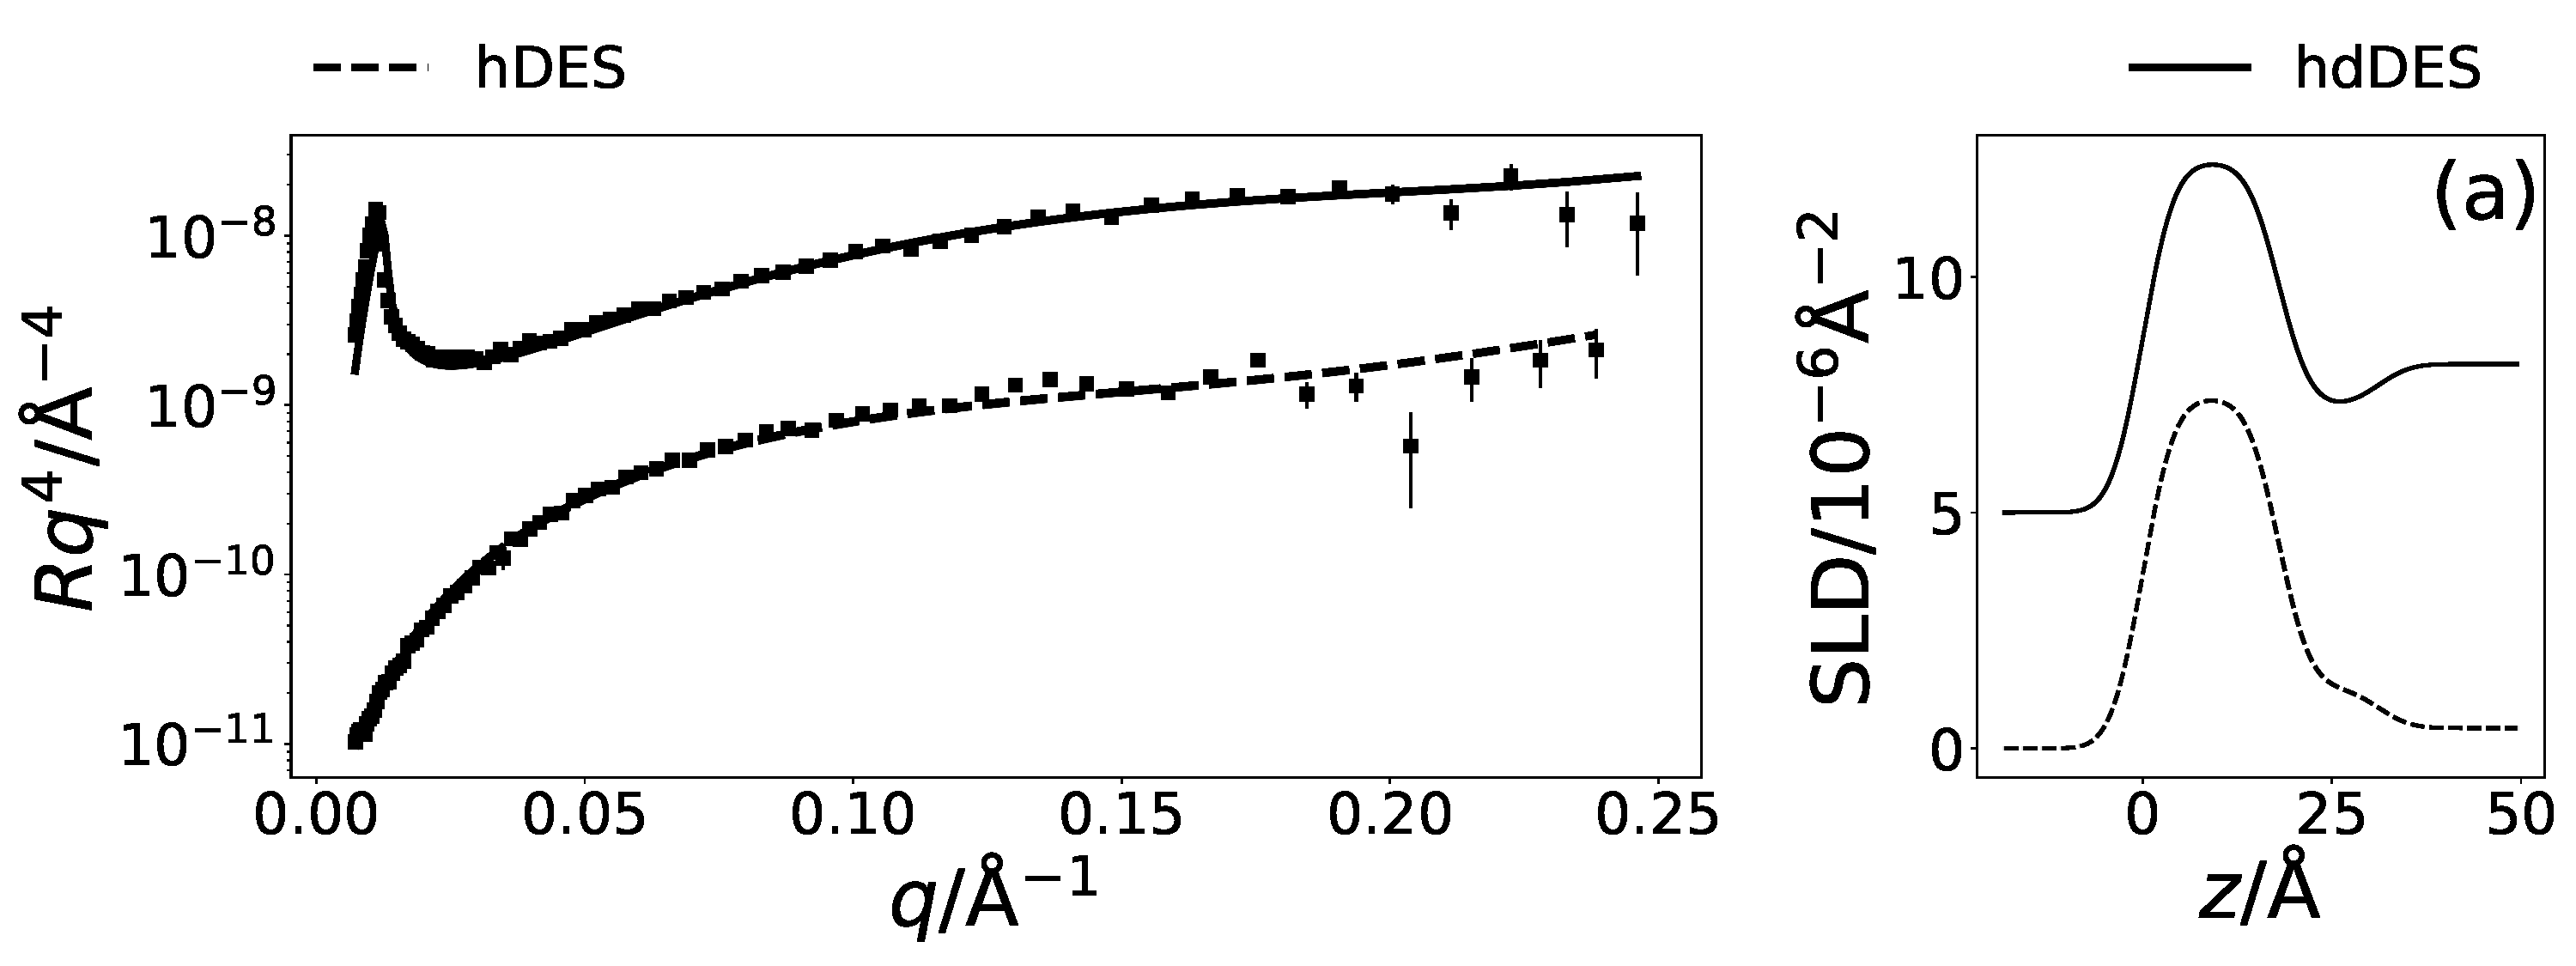
\includegraphics[width=0.9\textwidth]{figures/dmpc_25n_ref_sld}
	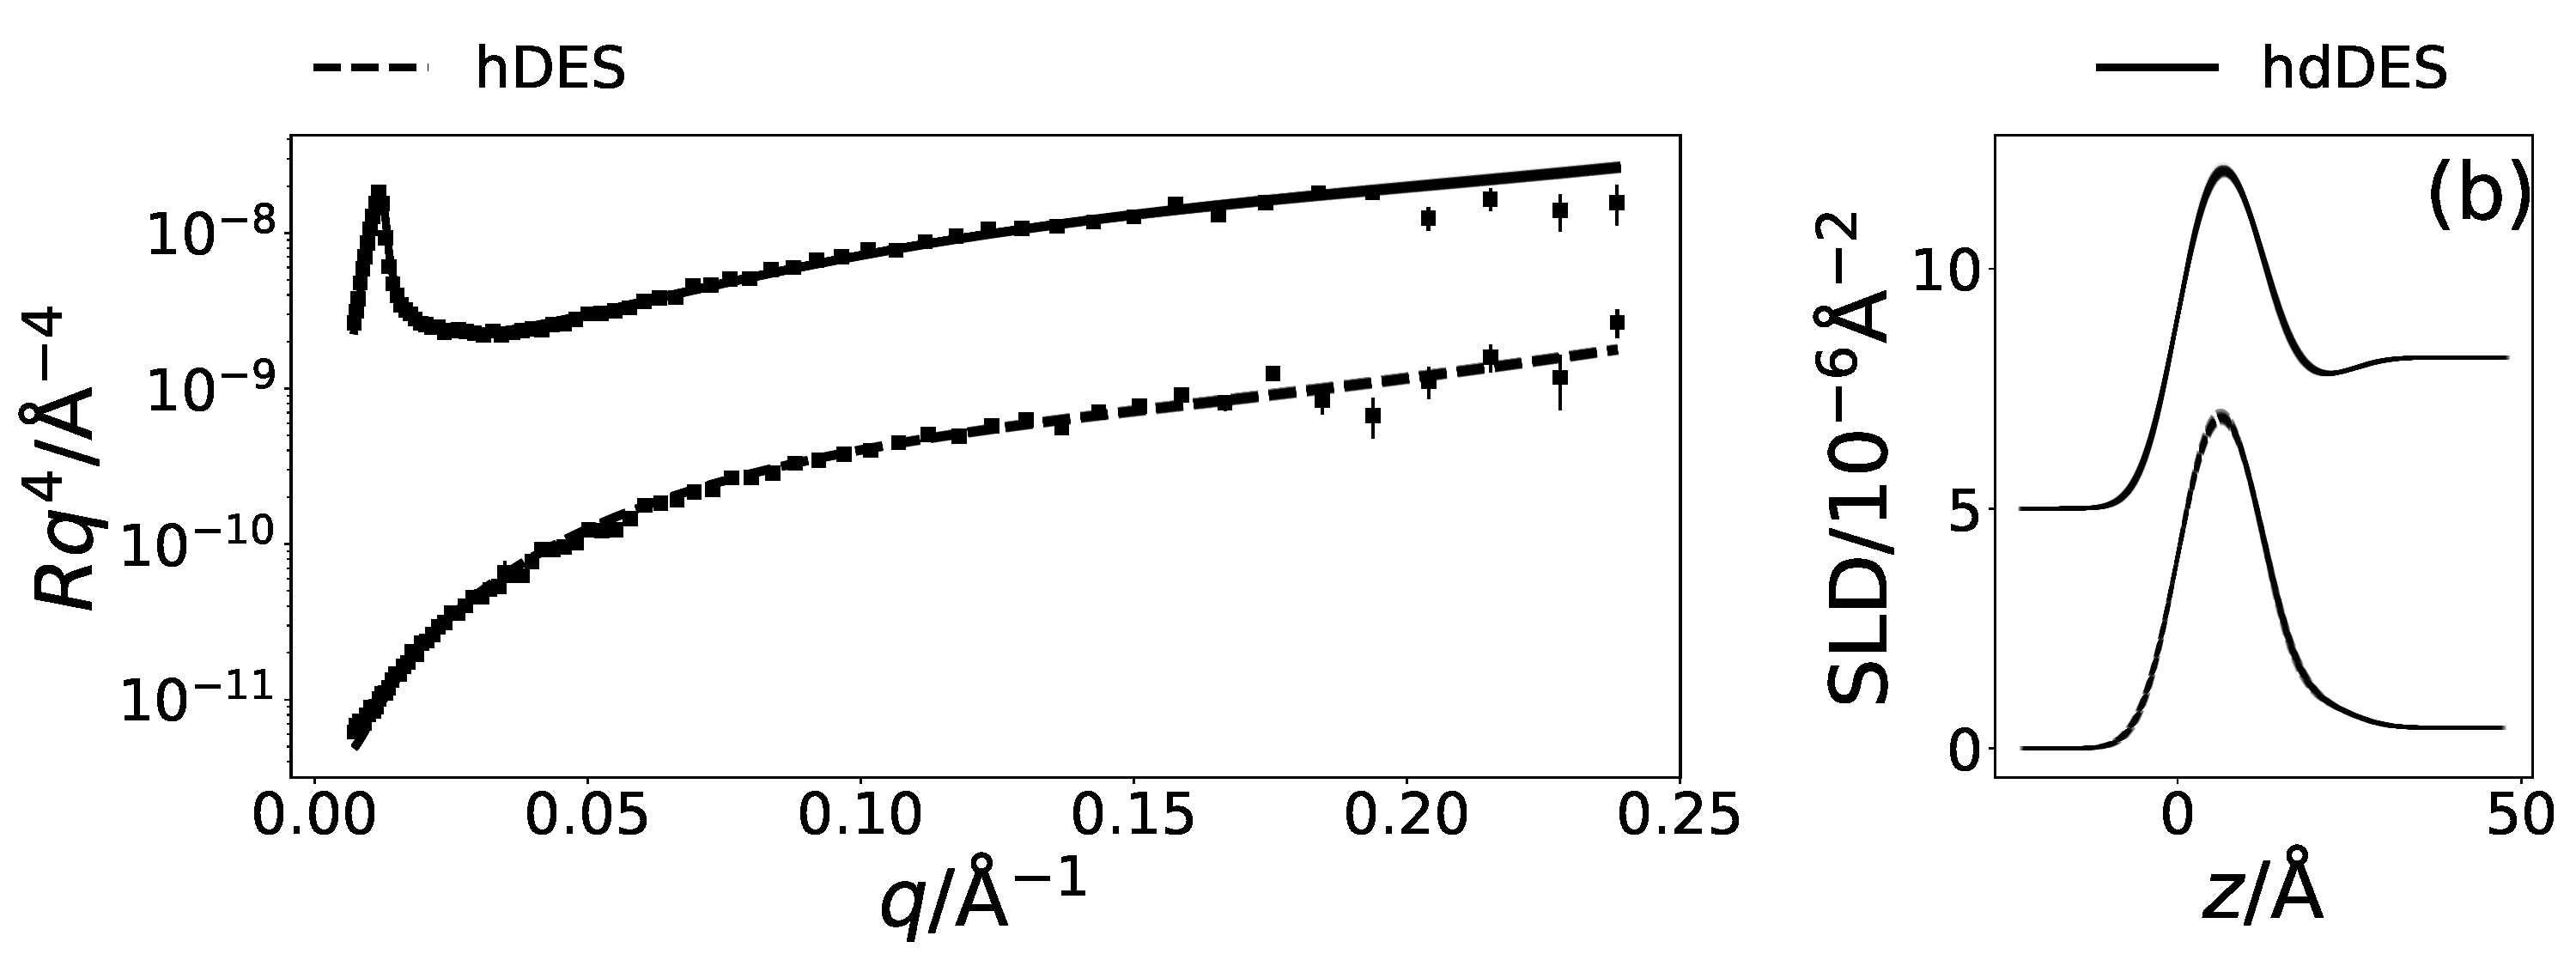
\includegraphics[width=0.9\textwidth]{figures/dppc_15n_ref_sld}
	\caption{The NR and SLD profiles at a surface pressure of (a) 25 mNm$^{-1}$ for two contrasts of DMPC, and (b) 15 mNm$^{-1}$ for two contrasts of DPPC. The NR profiles have been offset in the $y$-axis by an order of magnitude and SLD profiles offset in the $y$-axis by \SI{5e-6}{\per\square\angstrom}, for clarity.}
	\label{fig:neutron}
\end{figure}

\begin{figure}[H]
	\centering
	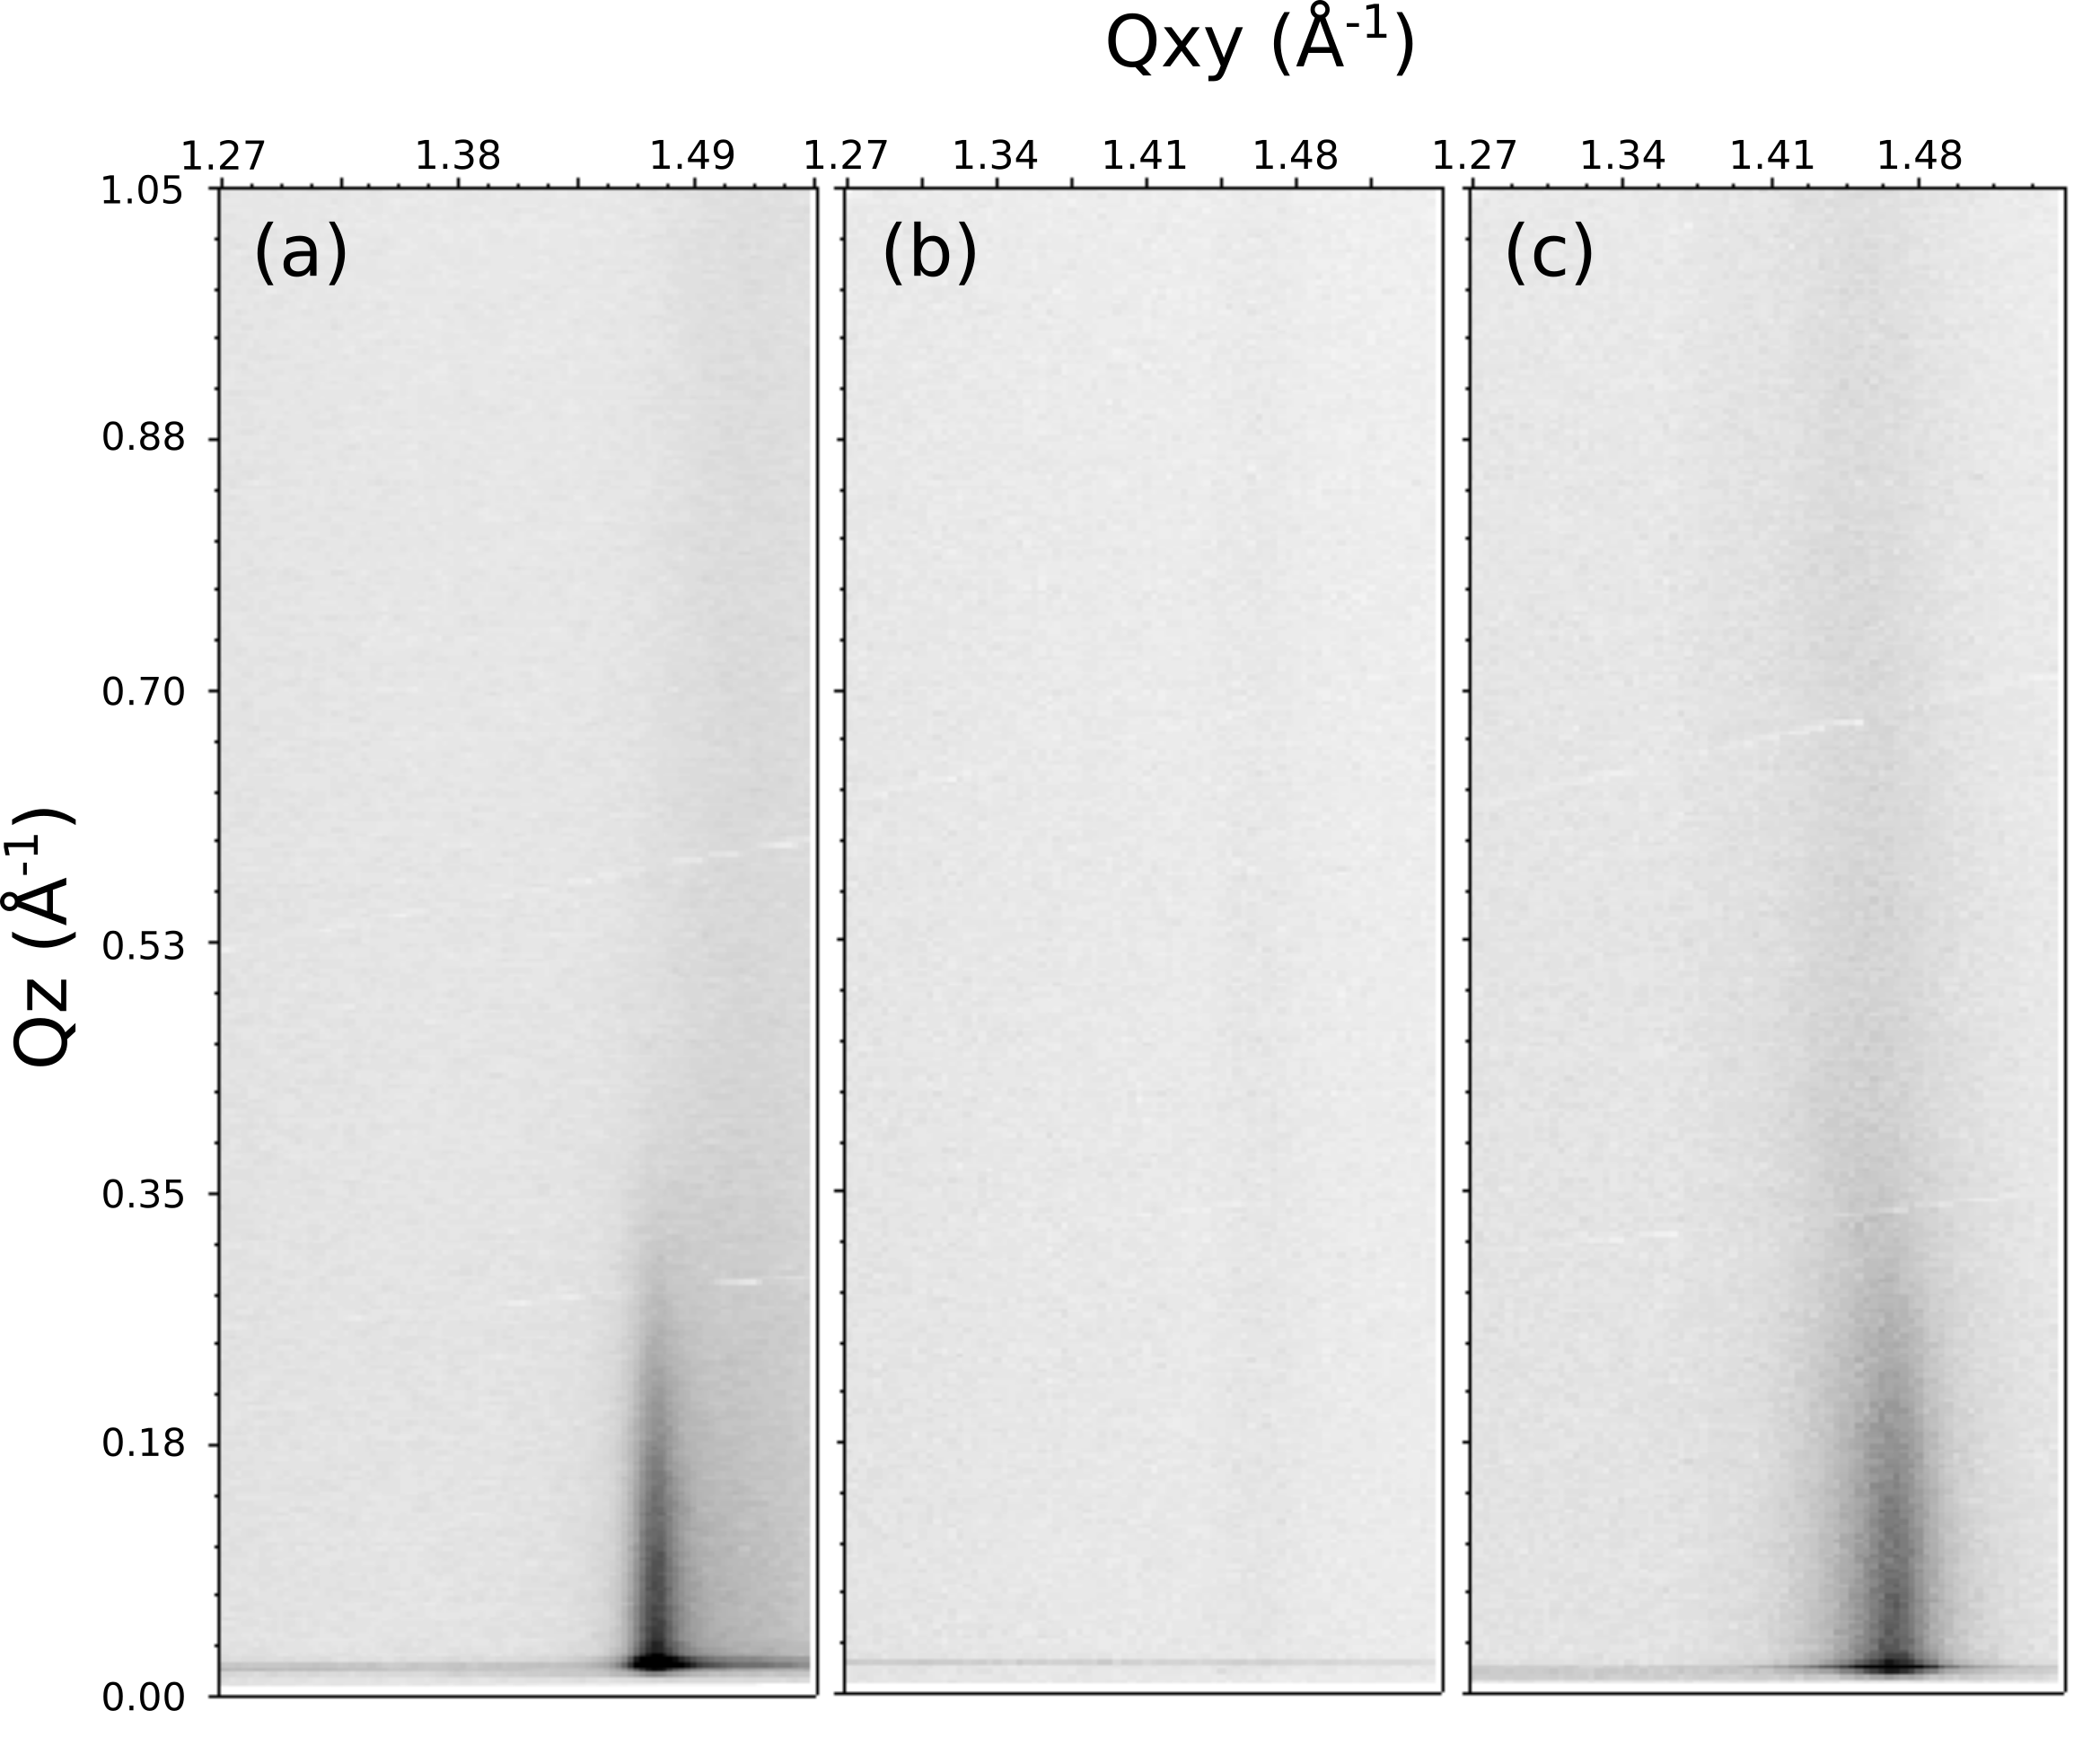
\includegraphics[width=0.50\textwidth]{figures/gixd}
	\caption{The GIXD pattern for (a) DPPC at \SI{30}{\milli\newton\per\meter} at \SI{22}{\celsius}, (b) DMPC at \SI{30}{\milli\newton\per\meter} at \SI{22}{\celsius}, and (c) DMPC at \SI{30}{\milli\newton\per\meter} at \SI{7}{\celsius}.}
	\label{fig:gixd}
\end{figure}

\begin{figure}[H]
	\centering
	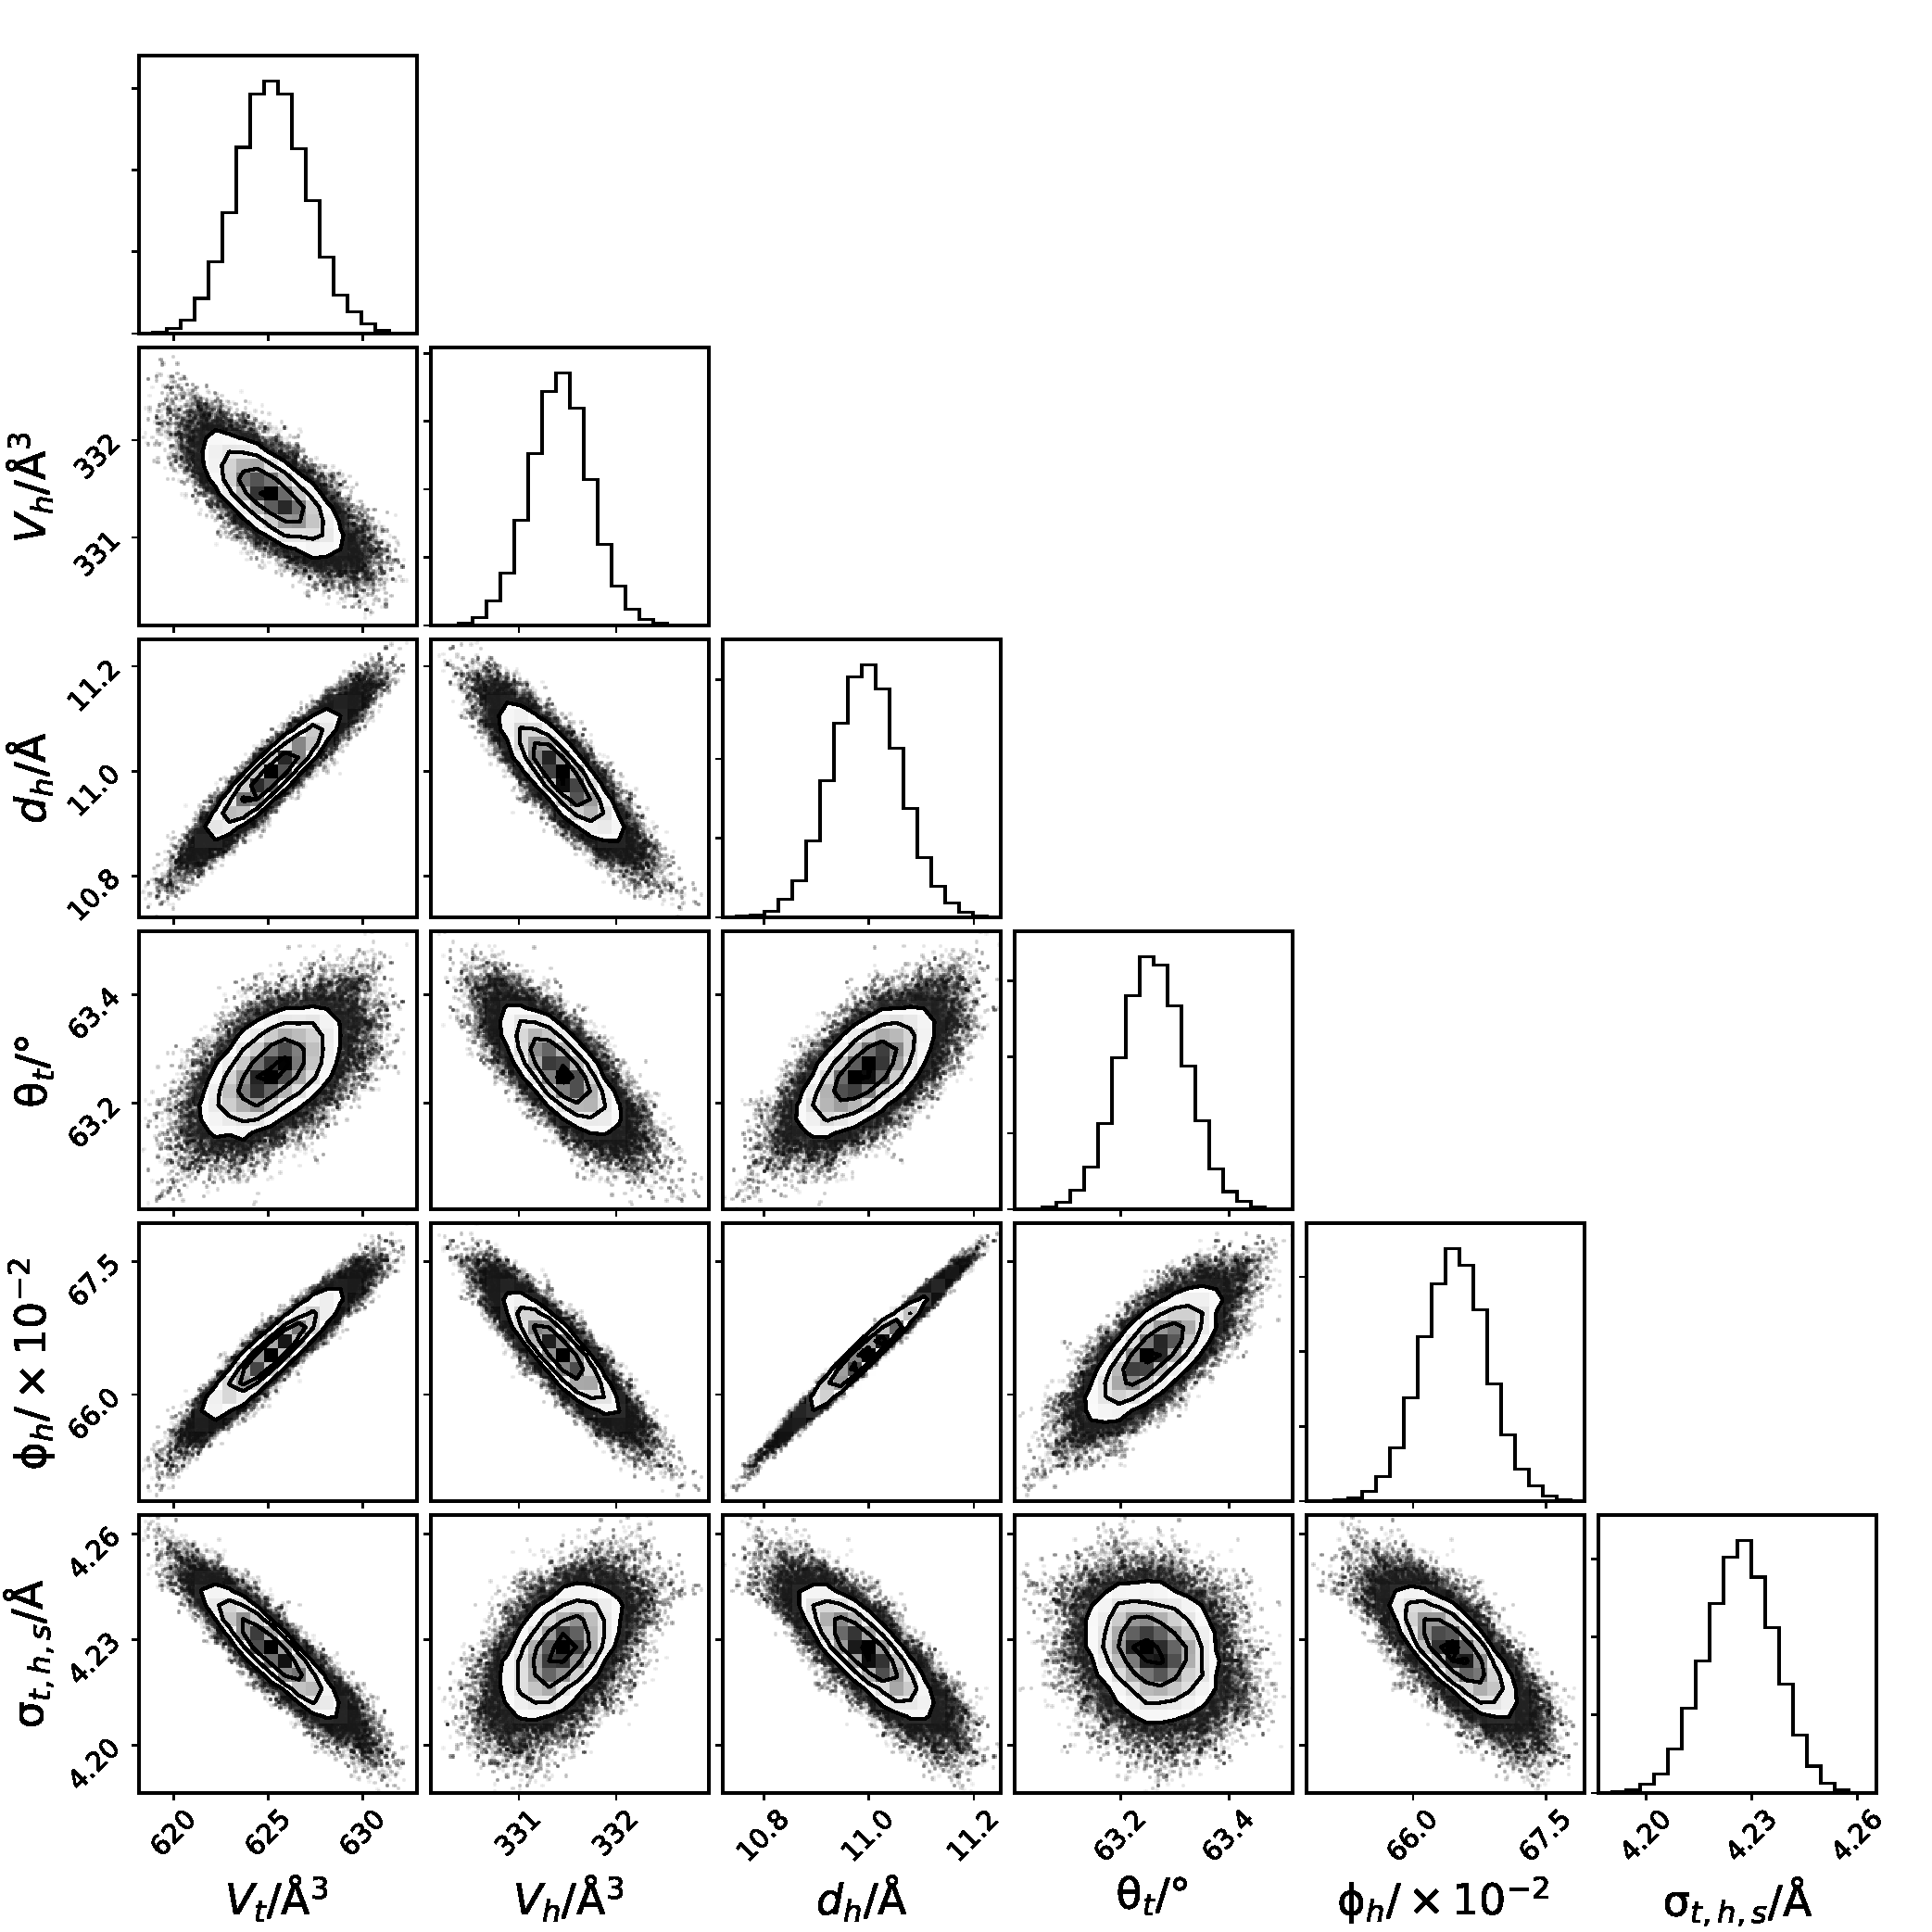
\includegraphics[width=0.50\textwidth]{figures/dlpc1_all_corner}
	\caption{The multi-parameter PDFs for the chemically-consistent model of DLPC X-ray reflectometry data at \SI{20}{\milli\newton\per\meter}.}
	\label{fig:dlpc1}
\end{figure}
\begin{figure}[H]
	\centering
	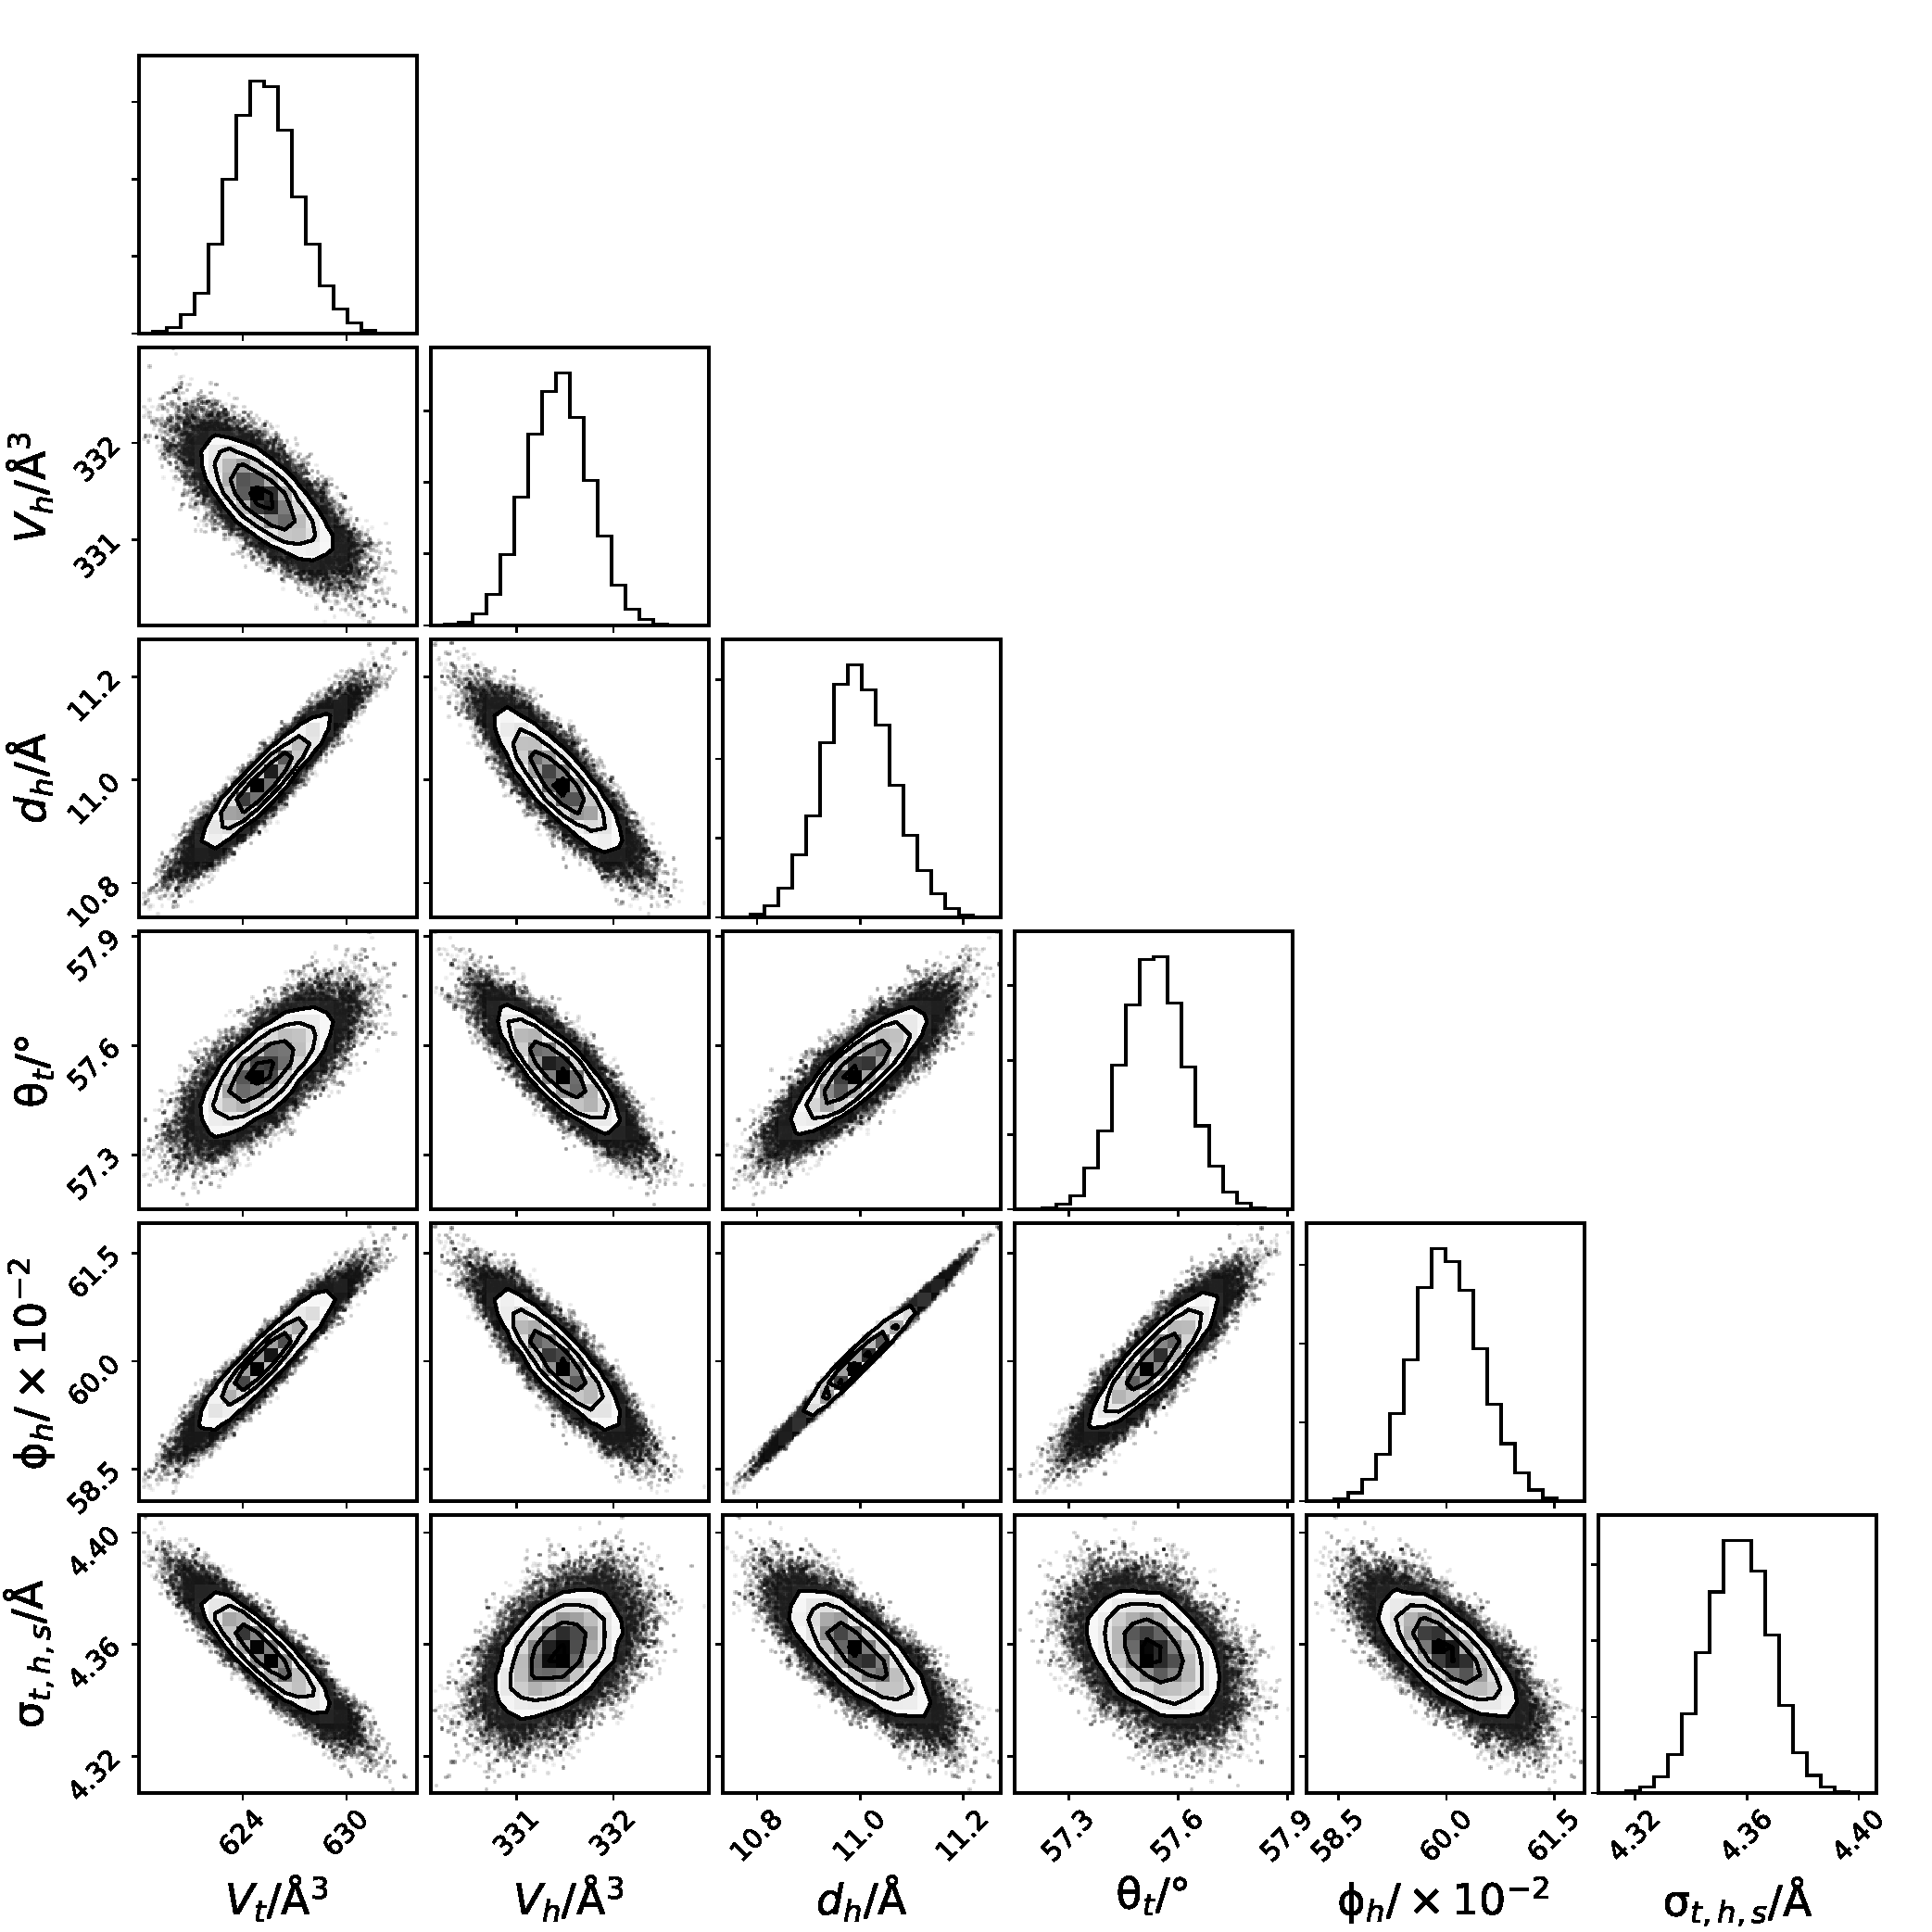
\includegraphics[width=0.50\textwidth]{figures/dlpc2_all_corner}
	\caption{The multi-parameter PDFs for the chemically-consistent model of DLPC X-ray reflectometry data at \SI{25}{\milli\newton\per\meter}.}
	\label{fig:dlpc2}
\end{figure}
\begin{figure}[H]
	\centering
	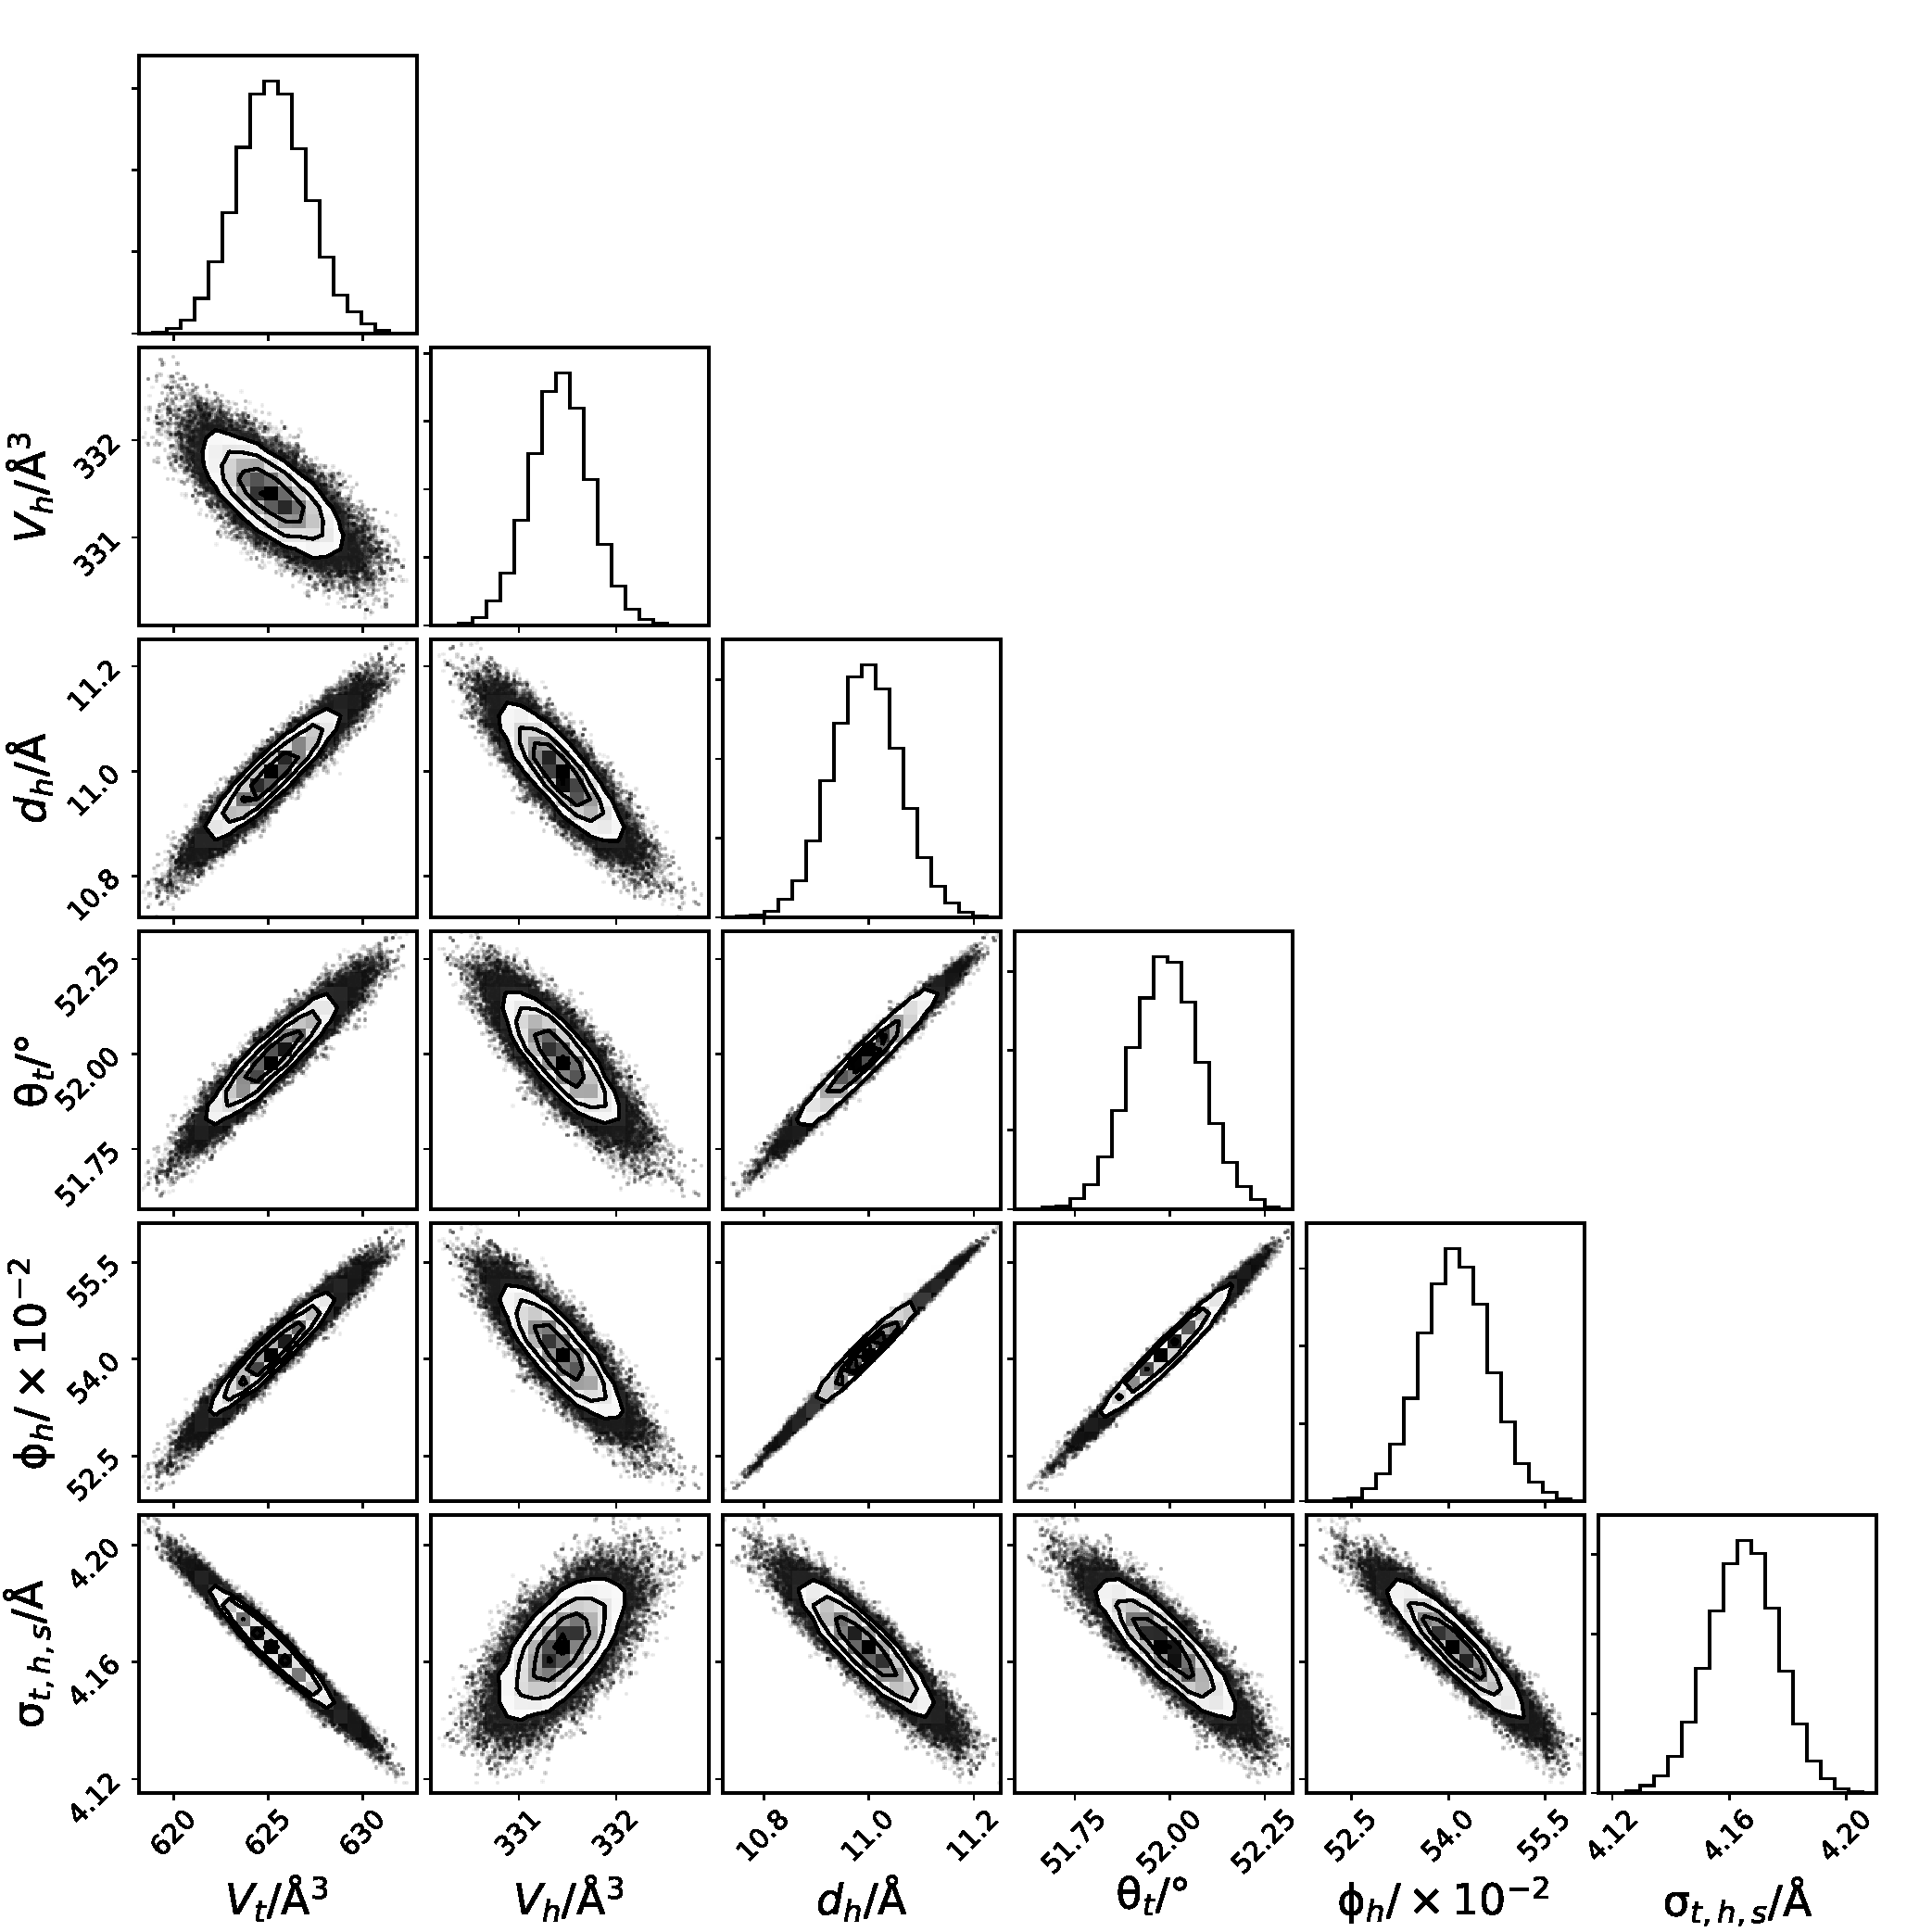
\includegraphics[width=0.50\textwidth]{figures/dlpc3_all_corner}
	\caption{The multi-parameter PDFs for the chemically-consistent model of DLPC X-ray reflectometry data at \SI{30}{\milli\newton\per\meter}.}
	\label{fig:dlpc3}
\end{figure}
\begin{figure}[H]
	\centering
	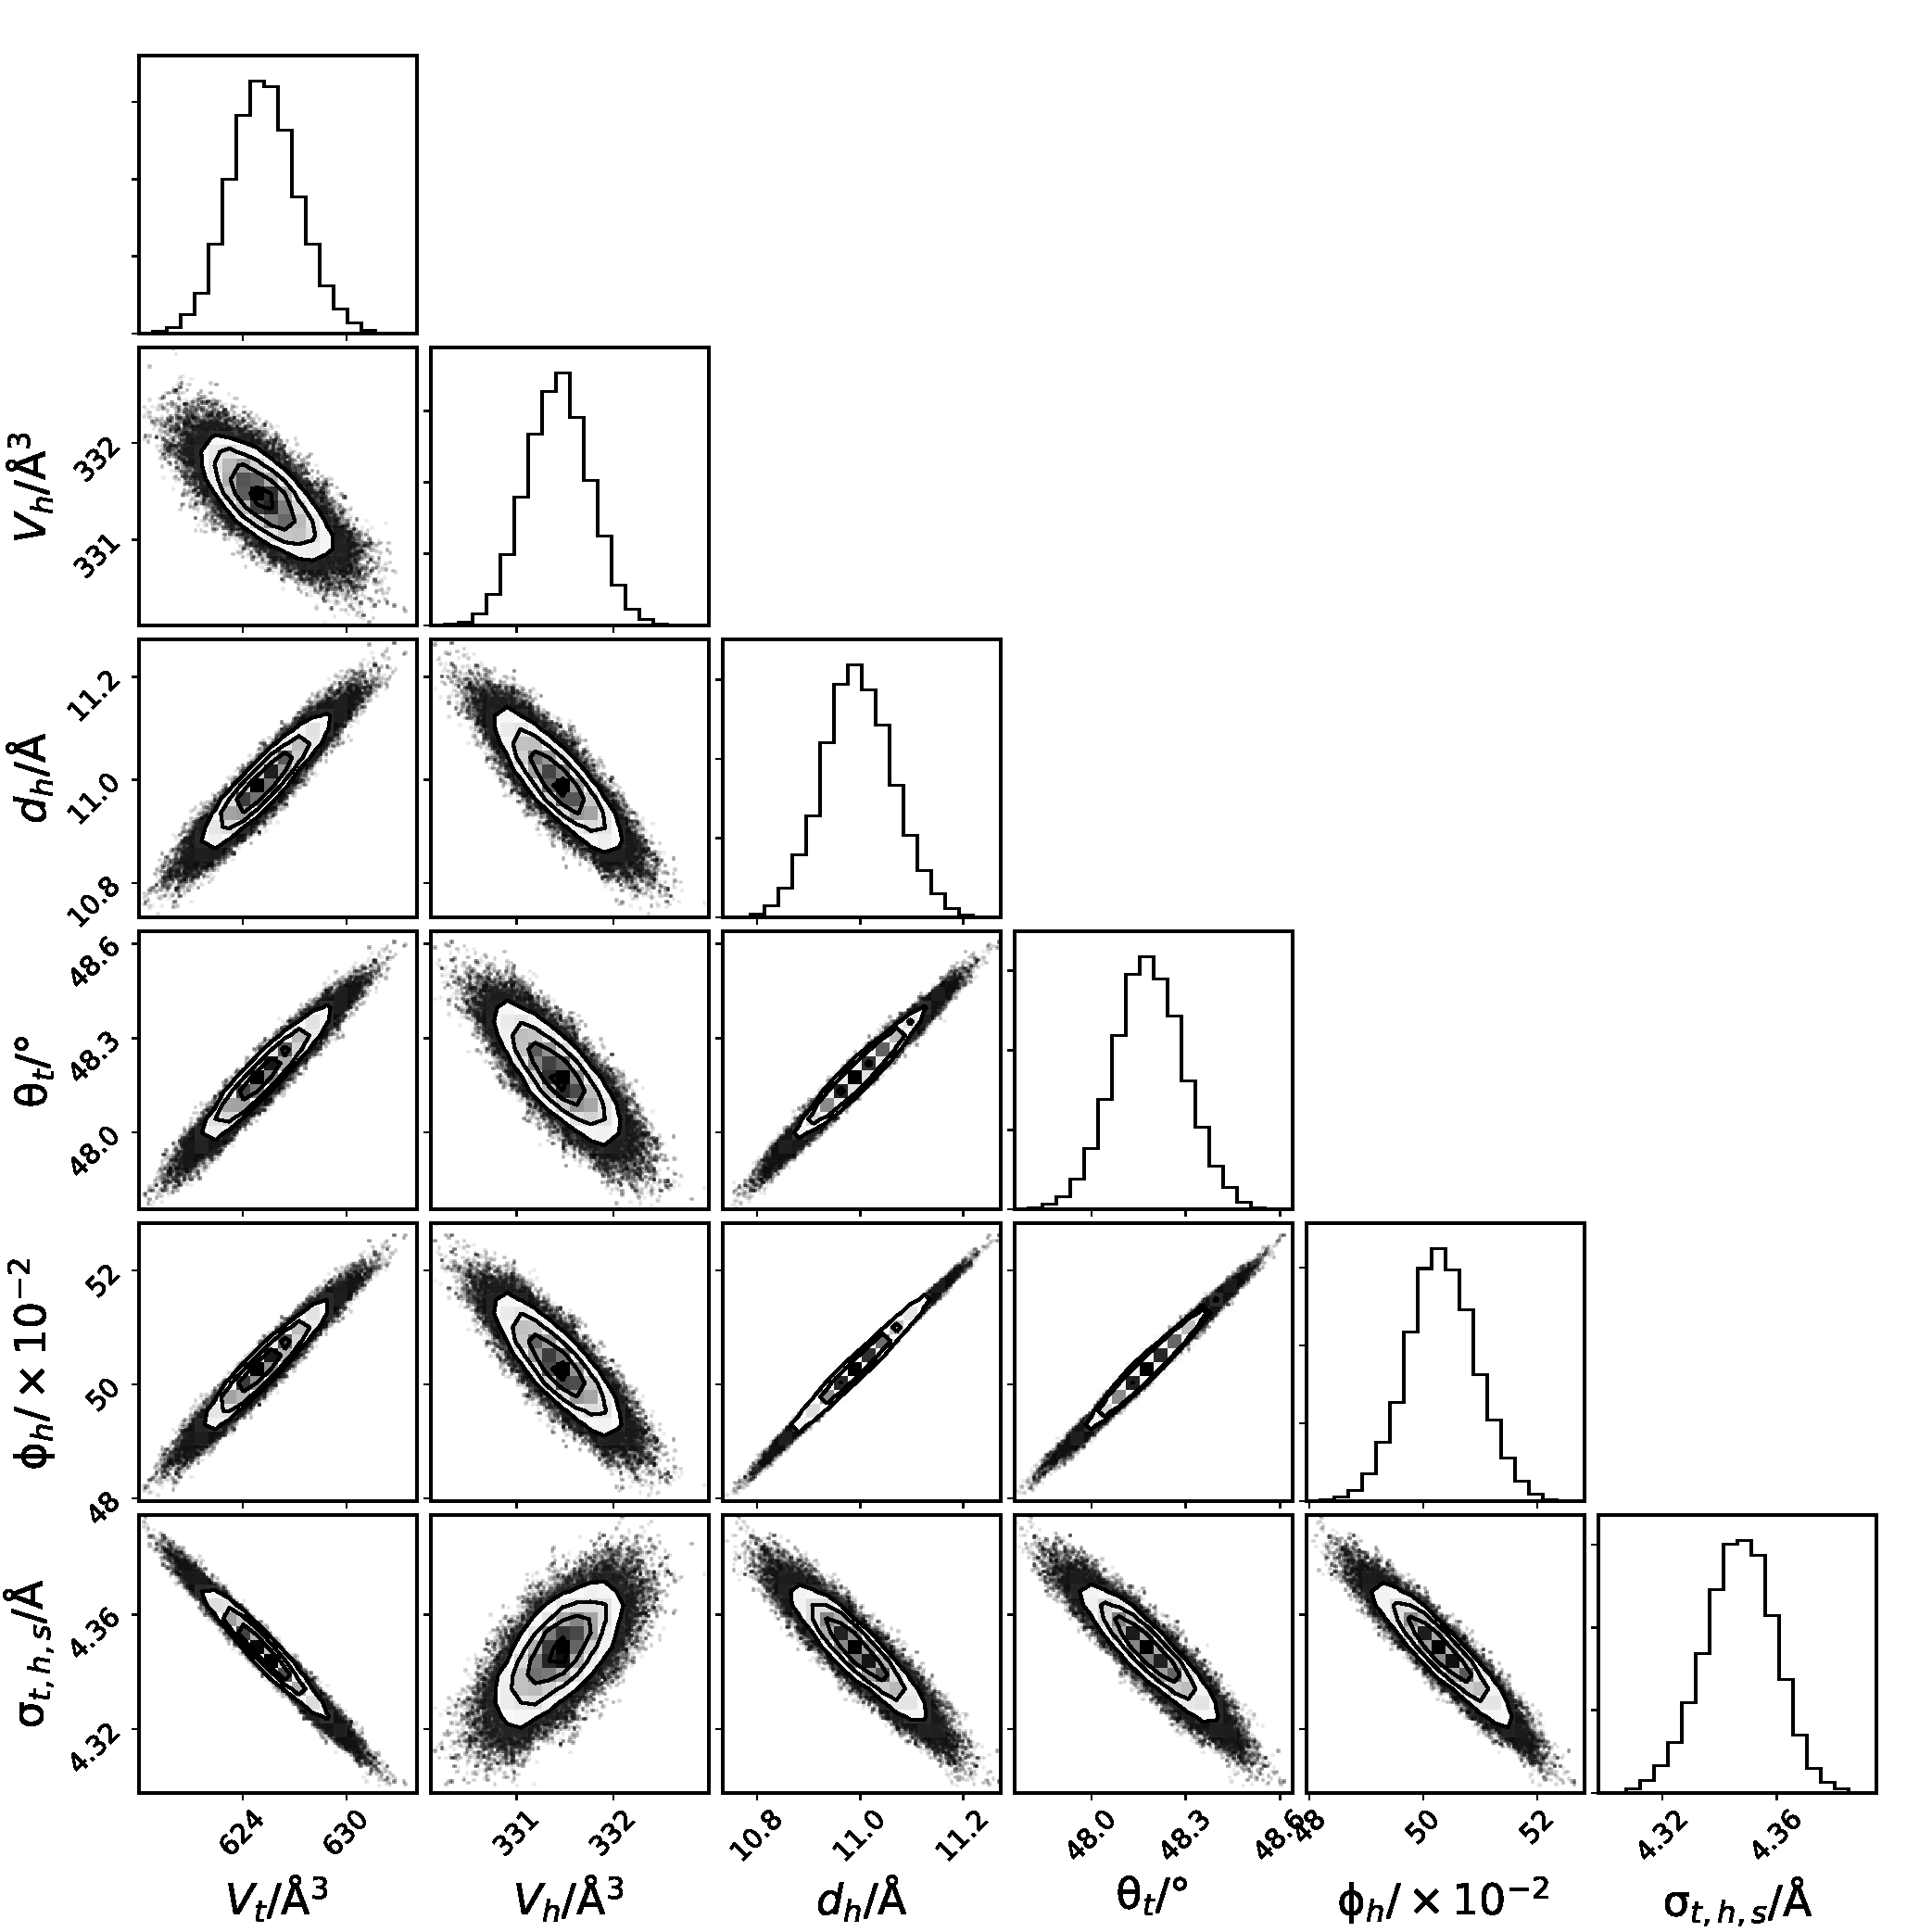
\includegraphics[width=0.50\textwidth]{figures/dlpc4_all_corner}
	\caption{The multi-parameter PDFs for the chemically-consistent model of DLPC X-ray reflectometry data at \SI{35}{\milli\newton\per\meter}.}
	\label{fig:dlpc4}
\end{figure}
\begin{figure}[H]
	\centering
	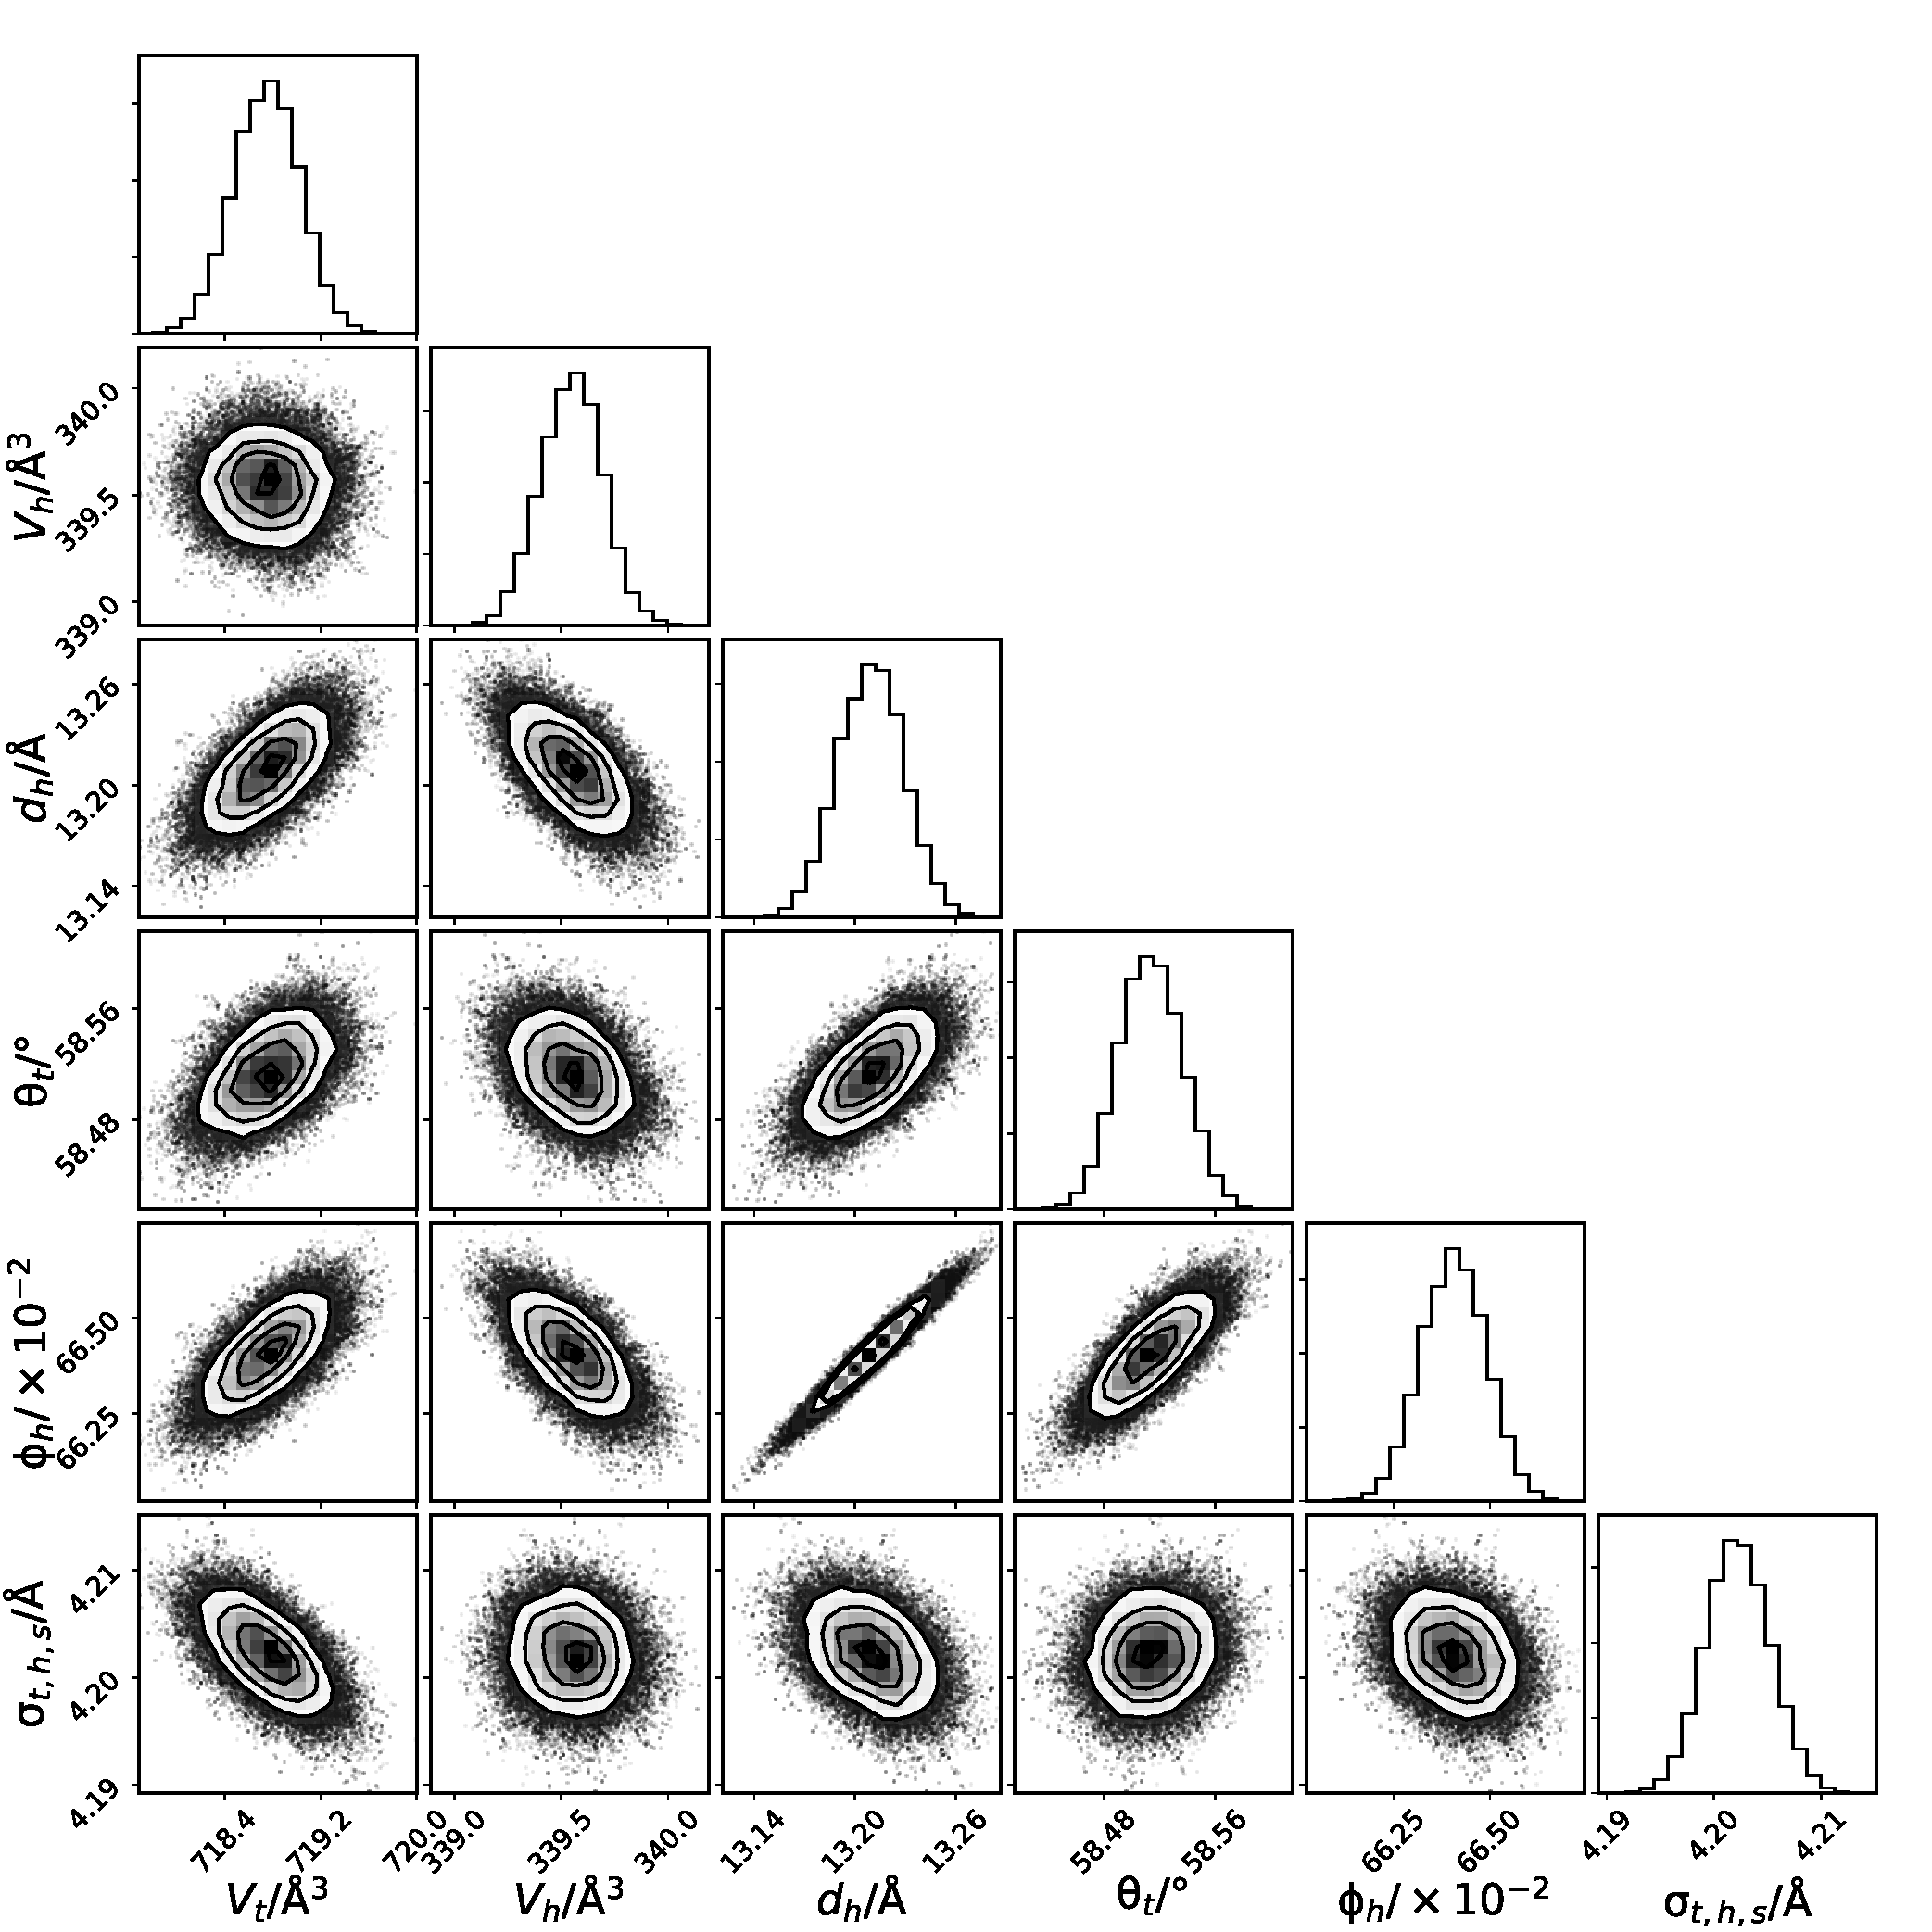
\includegraphics[width=0.50\textwidth]{figures/dmpc1_all_corner}
	\caption{The multi-parameter PDFs for the chemically-consistent model of DMPC X-ray reflectometry data at \SI{20}{\milli\newton\per\meter}.}
	\label{fig:dmpc1}
\end{figure}
\begin{figure}[H]
	\centering
	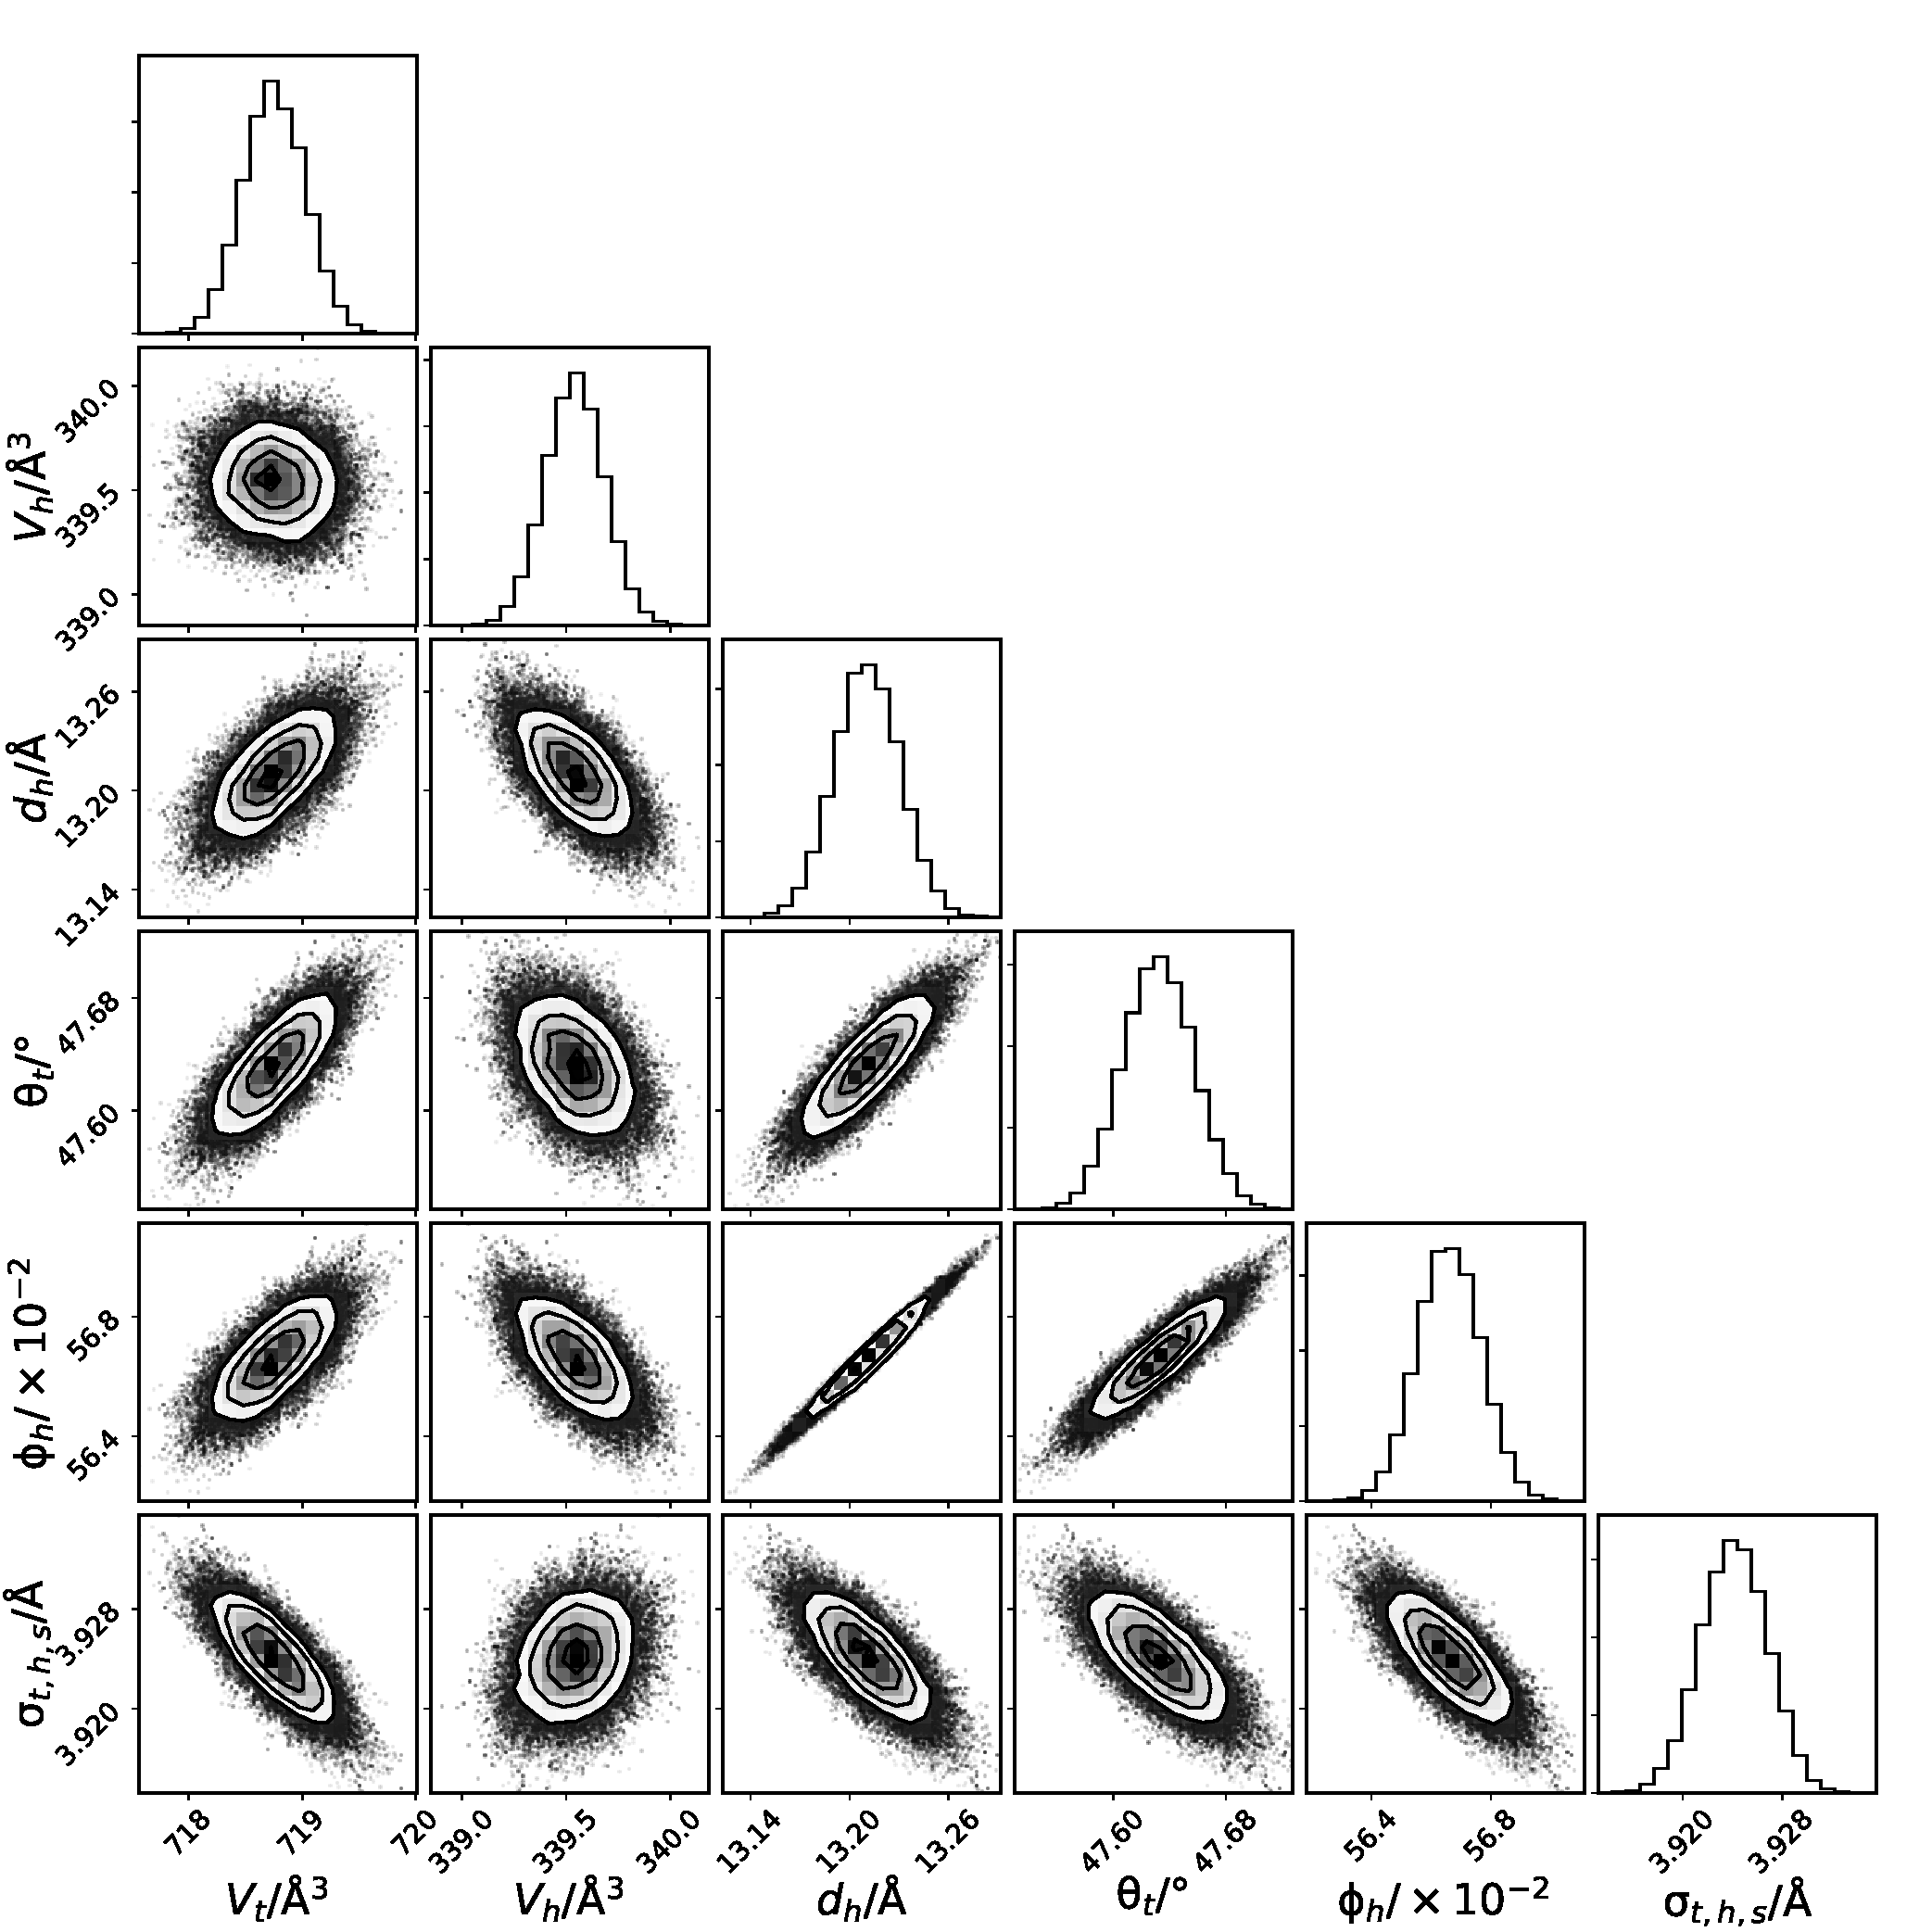
\includegraphics[width=0.50\textwidth]{figures/dmpc2_all_corner}
	\caption{The multi-parameter PDFs for the chemically-consistent model of DMPC X-ray reflectometry data at \SI{25}{\milli\newton\per\meter}.}
	\label{fig:dmpc2}
\end{figure}
\begin{figure}[H]
	\centering
	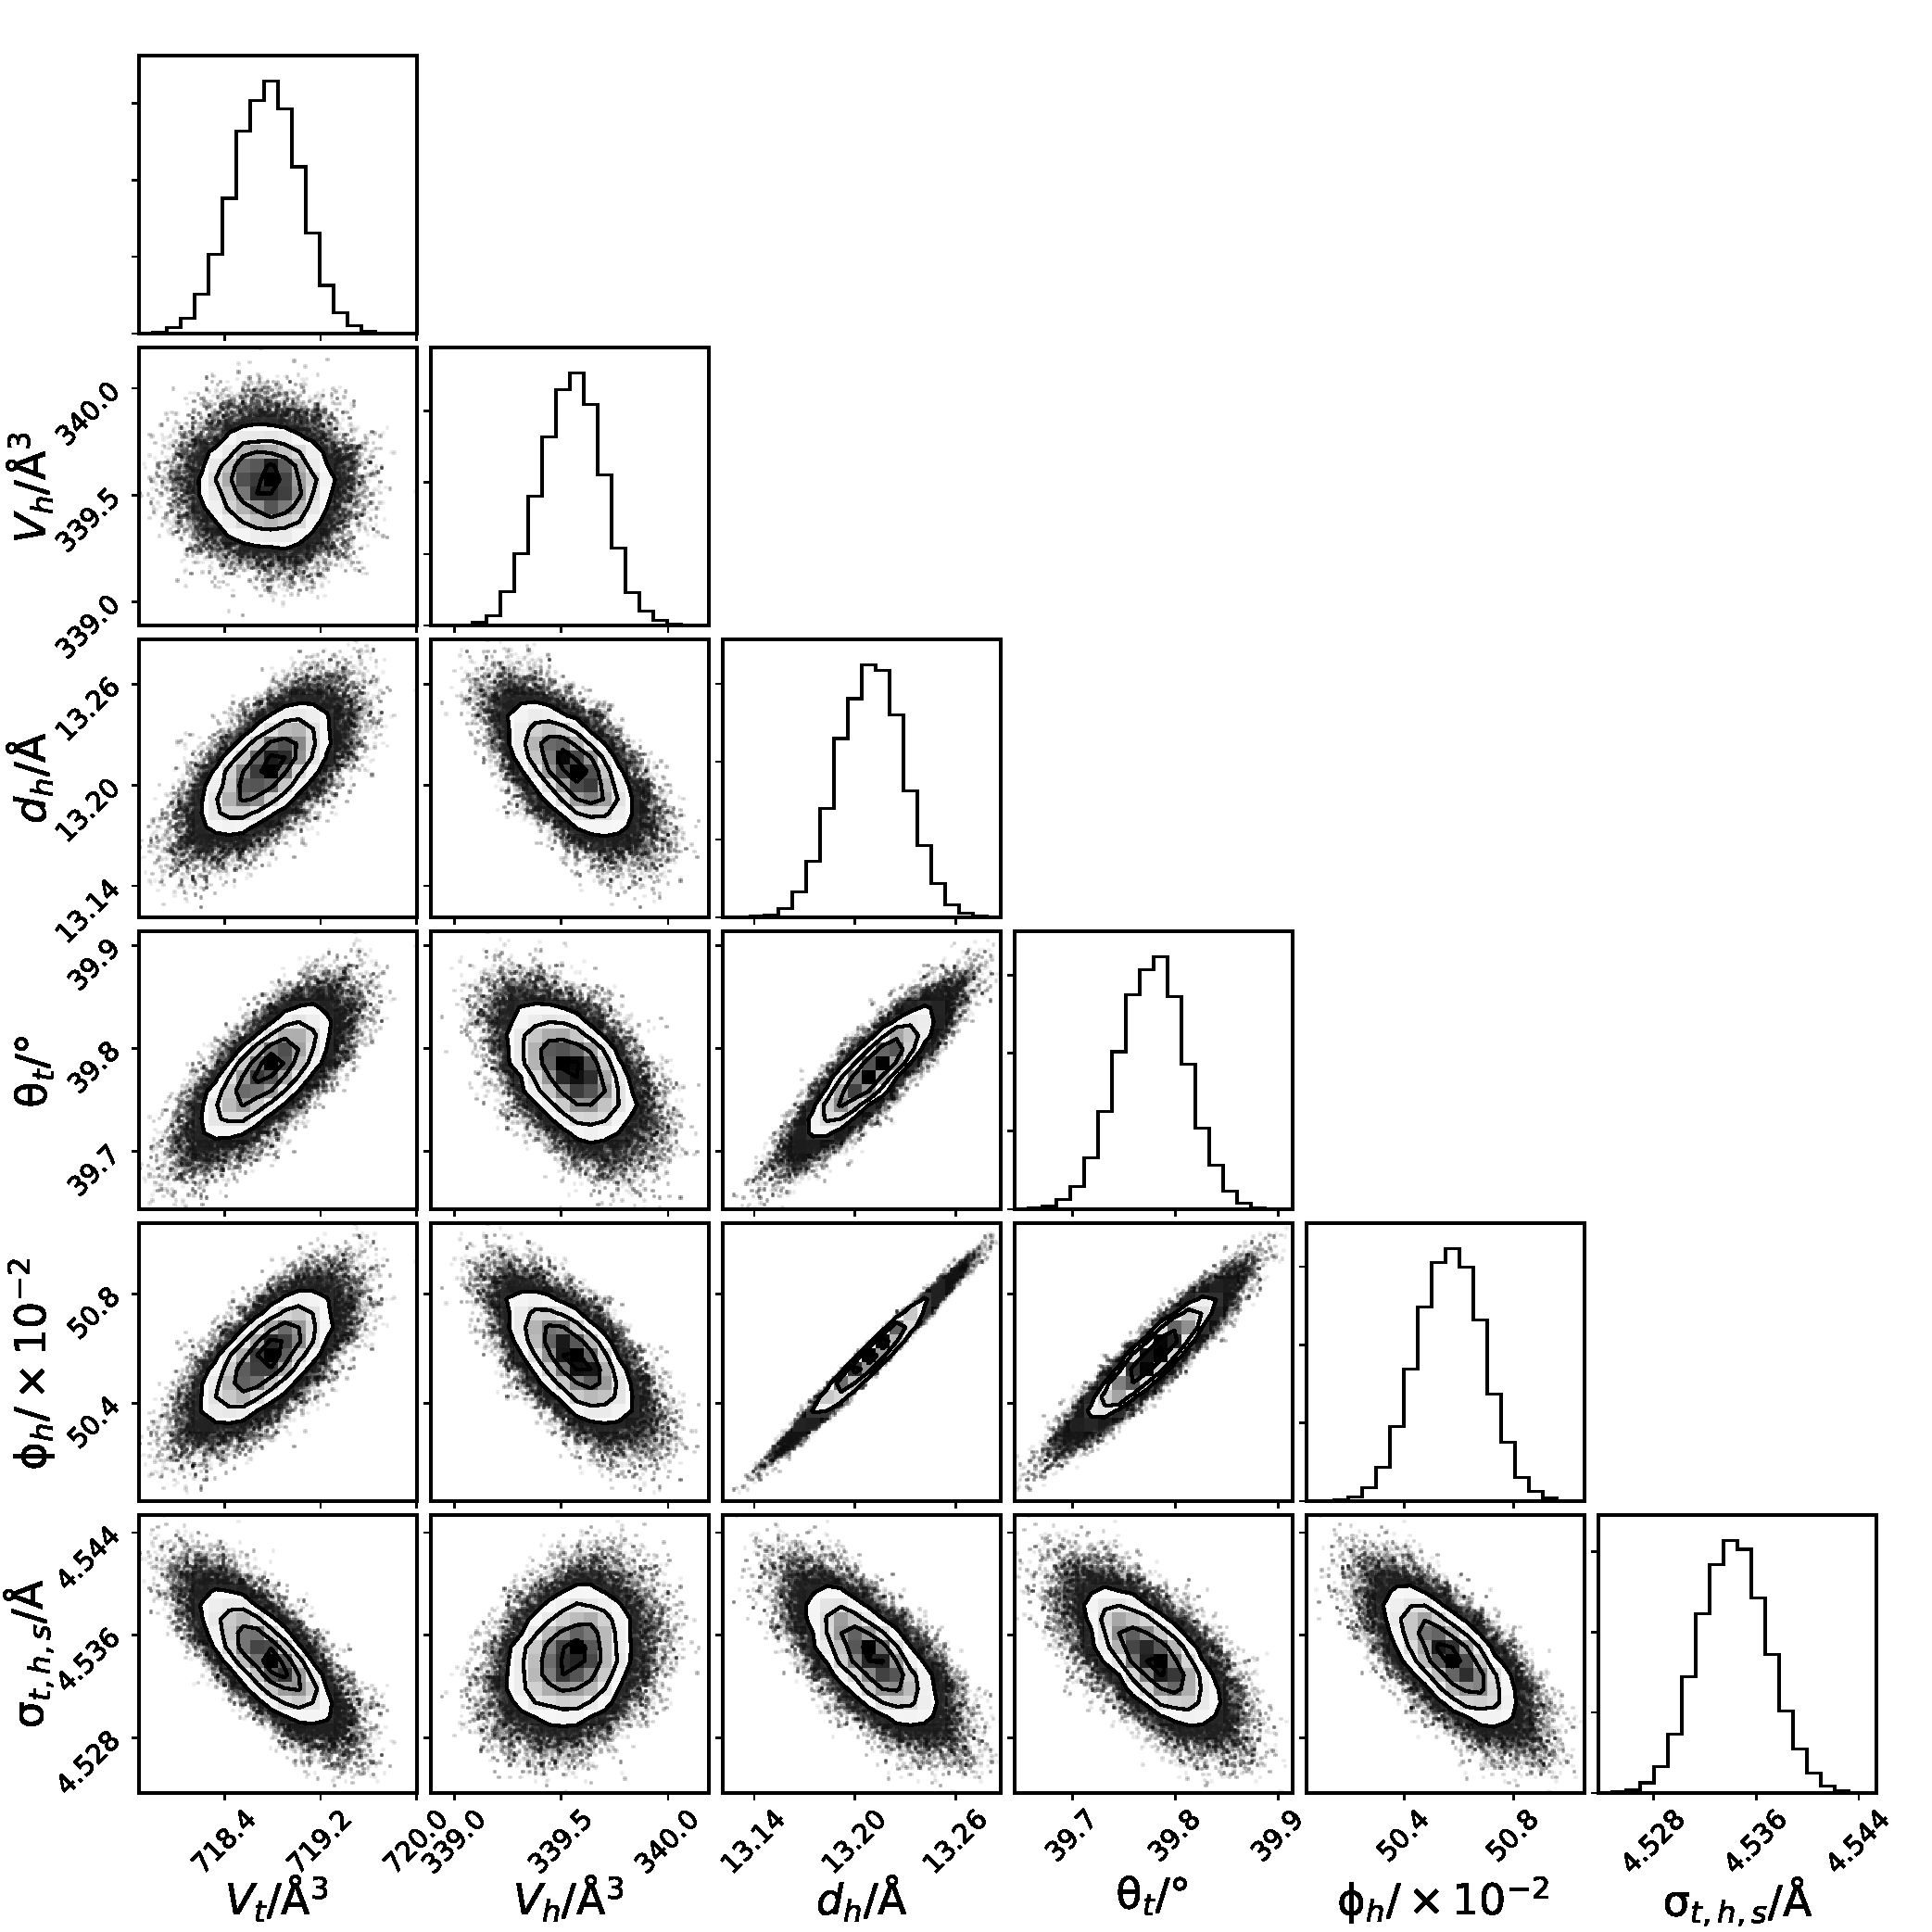
\includegraphics[width=0.50\textwidth]{figures/dmpc4_all_corner}
	\caption{The multi-parameter PDFs for the chemically-consistent model of DMPC X-ray reflectometry data at \SI{40}{\milli\newton\per\meter}.}
	\label{fig:dmpc4}
\end{figure}
\begin{figure}[H]
	\centering
	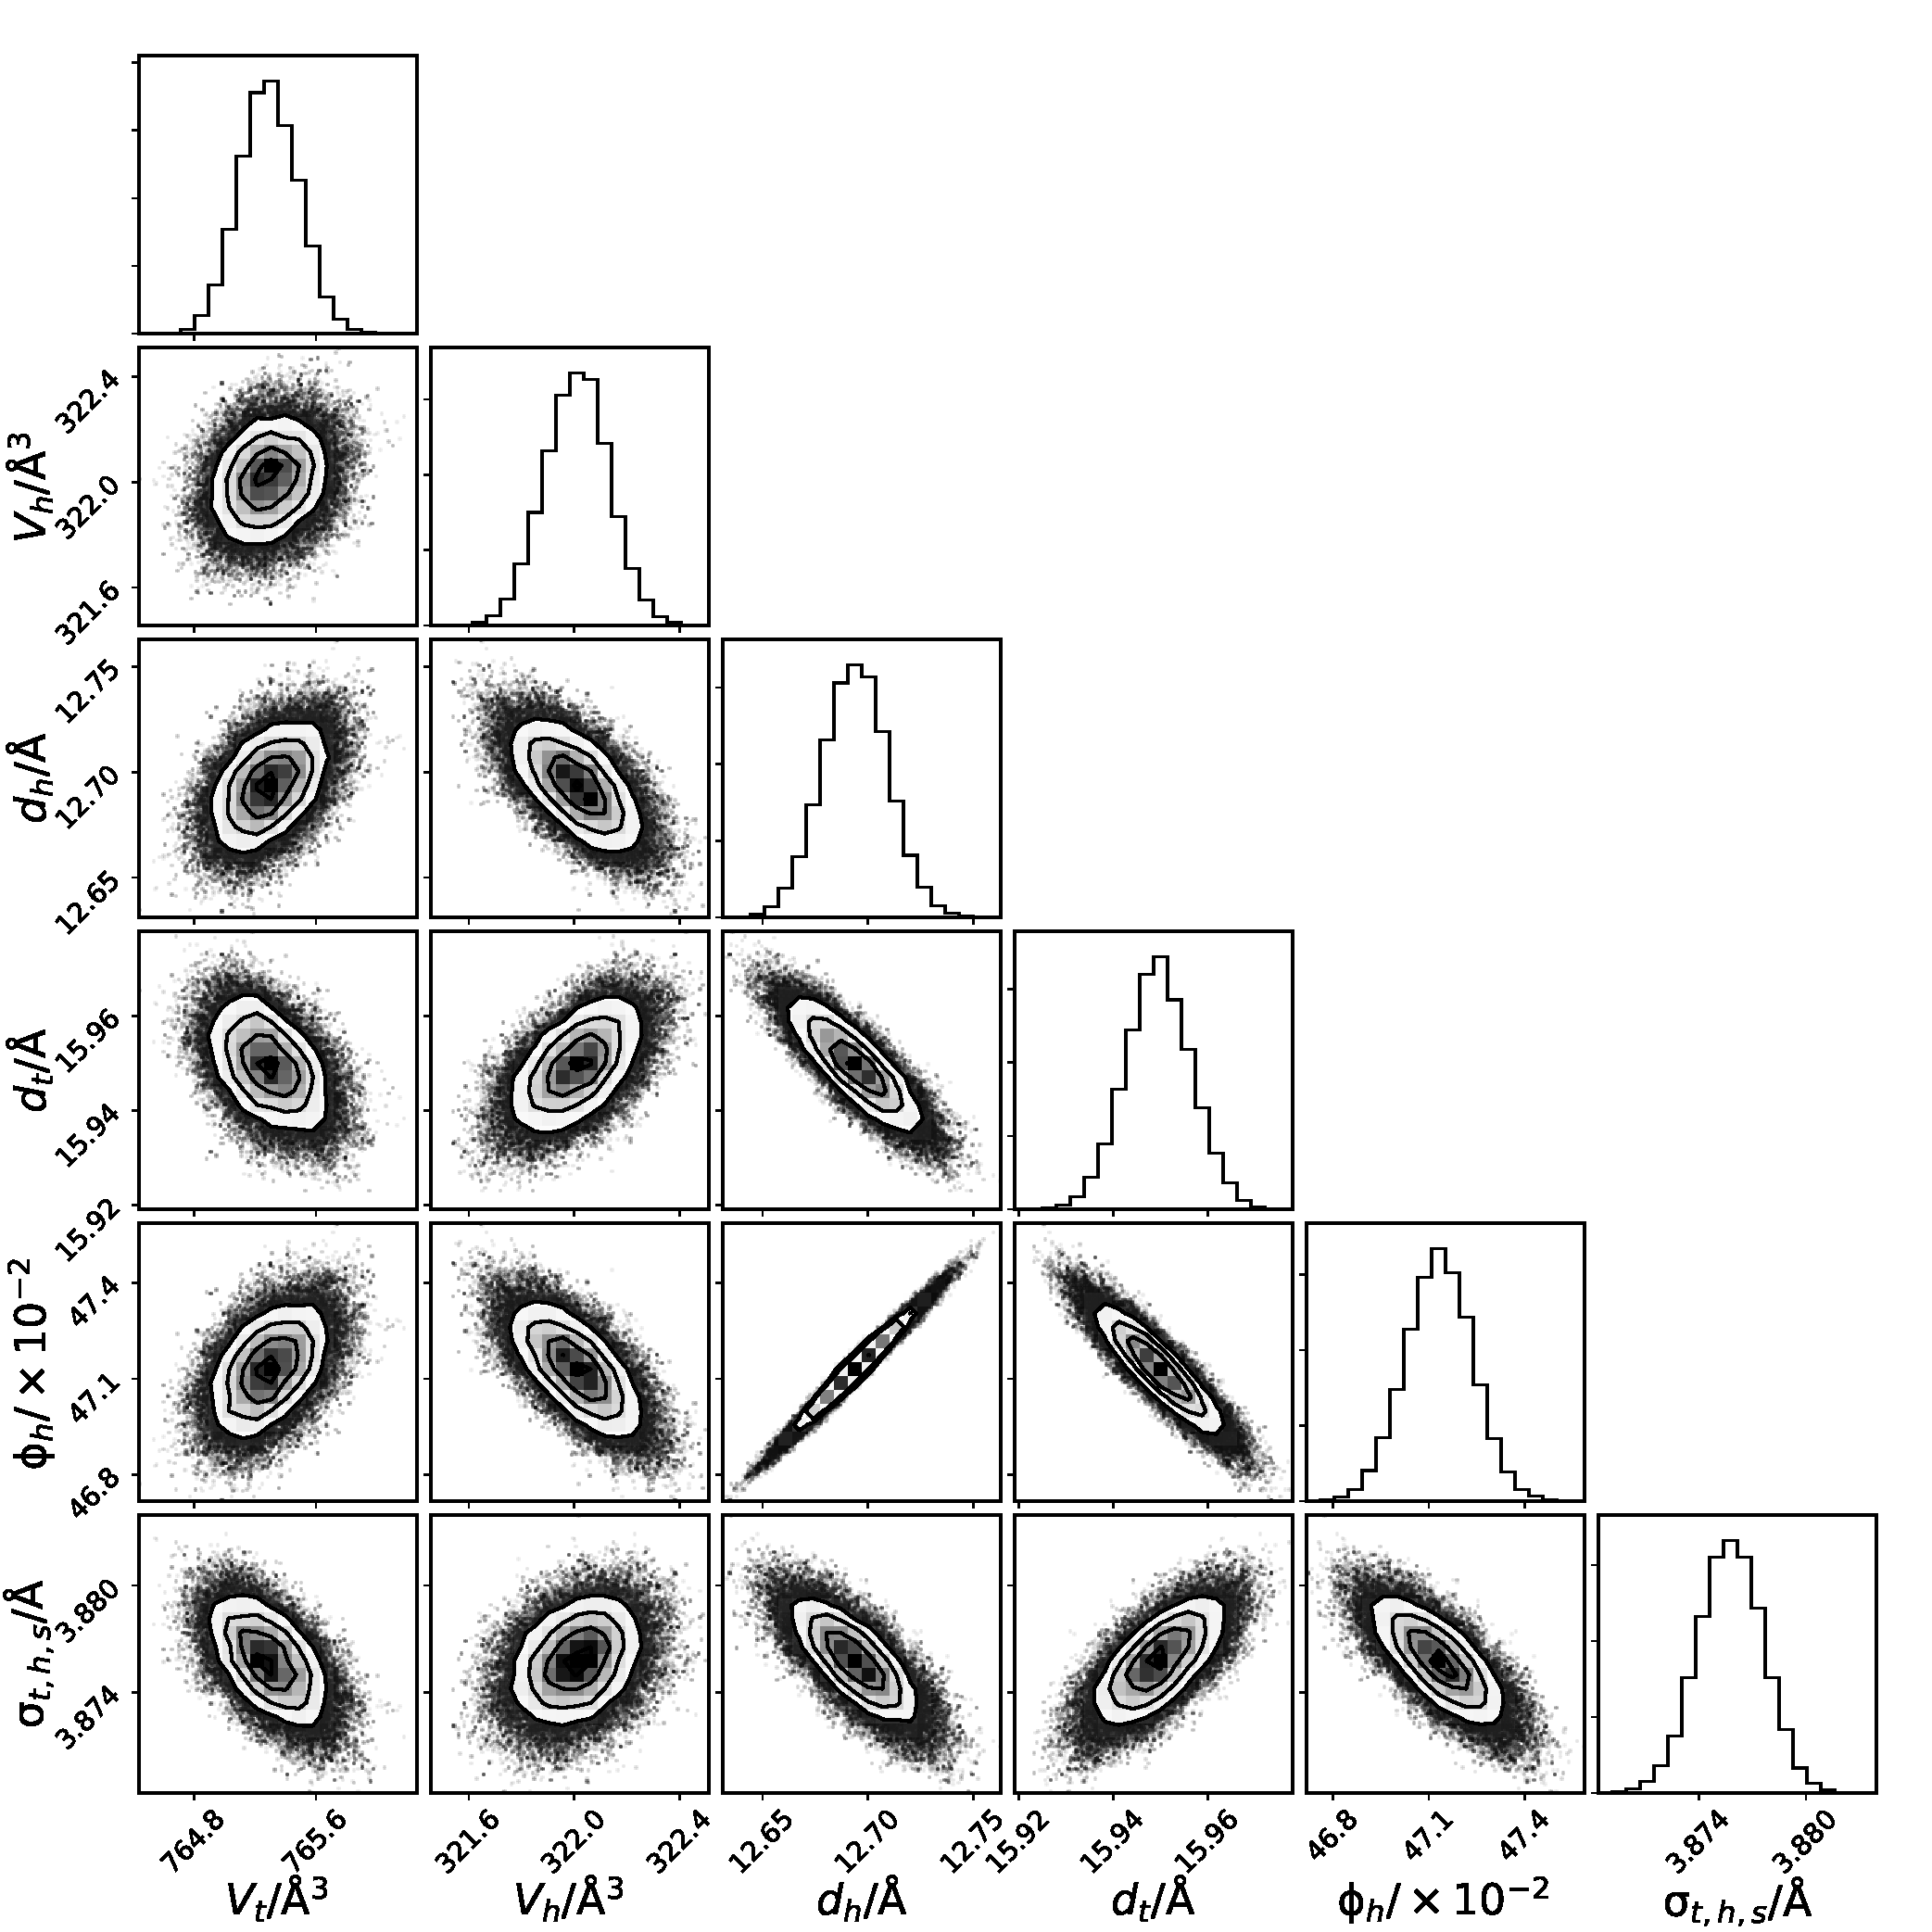
\includegraphics[width=0.50\textwidth]{figures/dppc1_all_corner}
	\caption{The multi-parameter PDFs for the chemically-consistent model of DPPC X-ray reflectometry data at \SI{15}{\milli\newton\per\meter}.}
	\label{fig:dppc1}
\end{figure}
\begin{figure}[H]
	\centering
	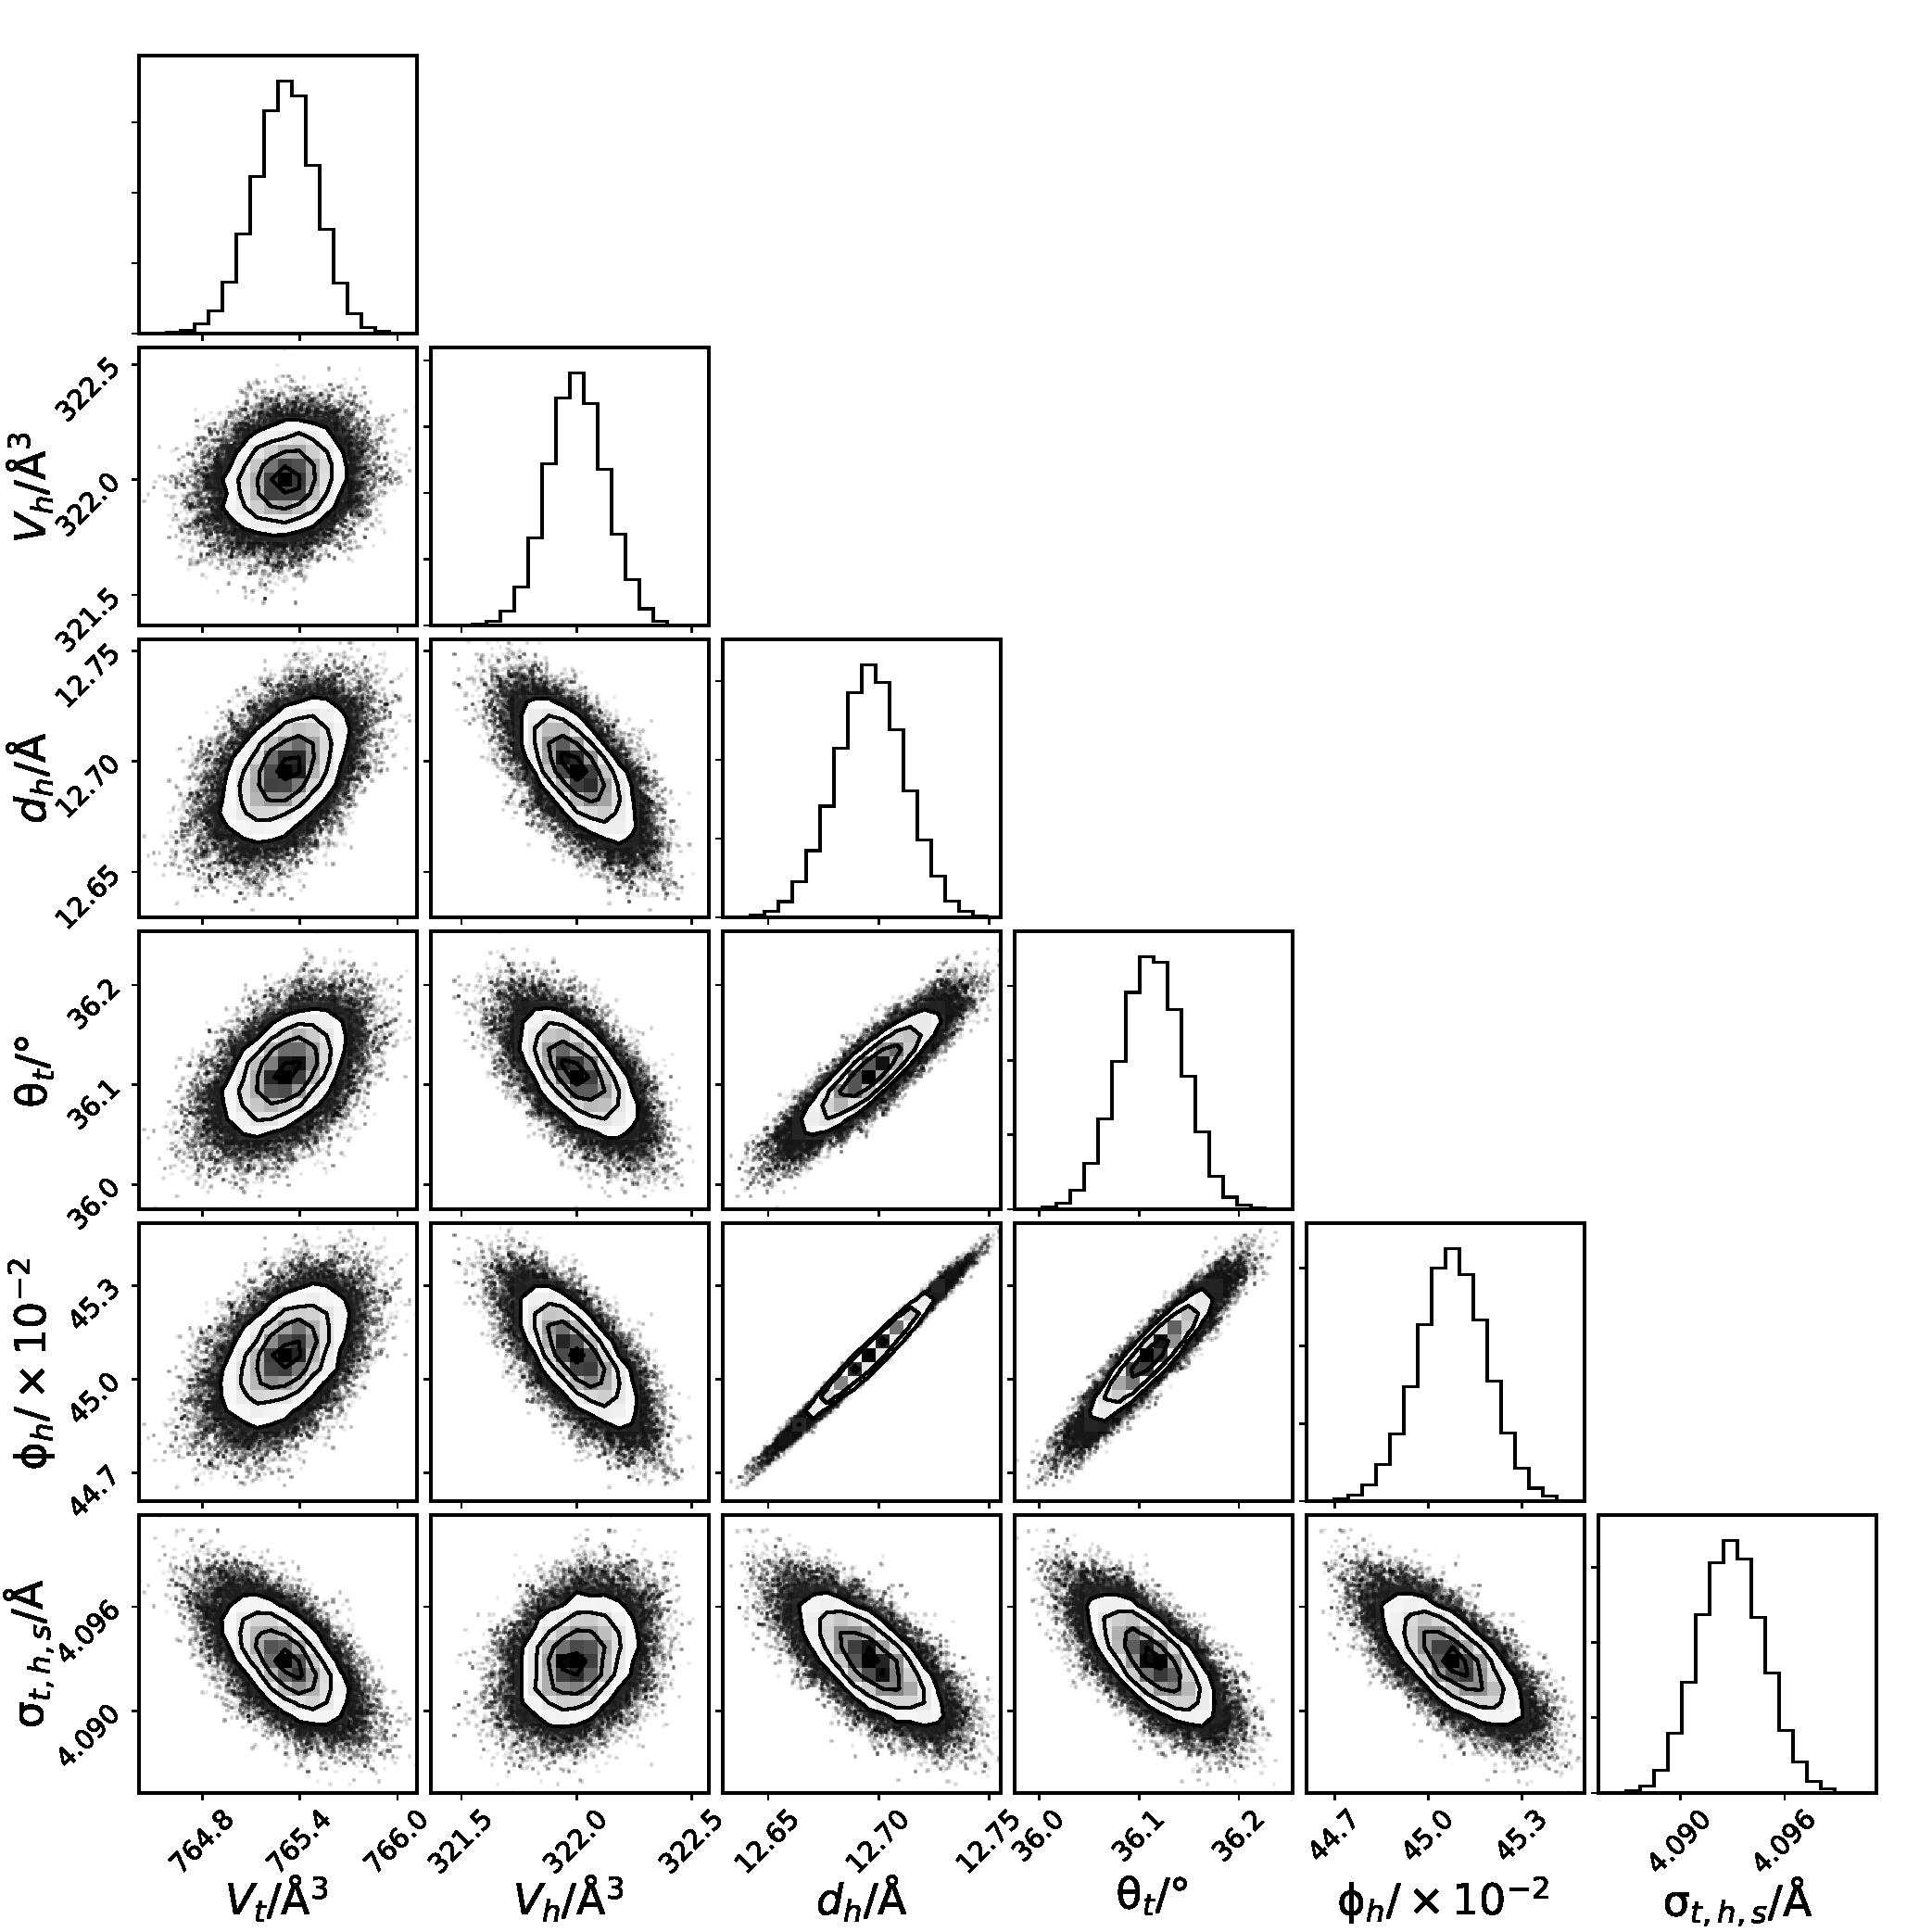
\includegraphics[width=0.50\textwidth]{figures/dppc2_all_corner}
	\caption{The multi-parameter PDFs for the chemically-consistent model of DPPC X-ray reflectometry data at \SI{20}{\milli\newton\per\meter}.}
	\label{fig:dppc2}
\end{figure}
\begin{figure}[H]
	\centering
	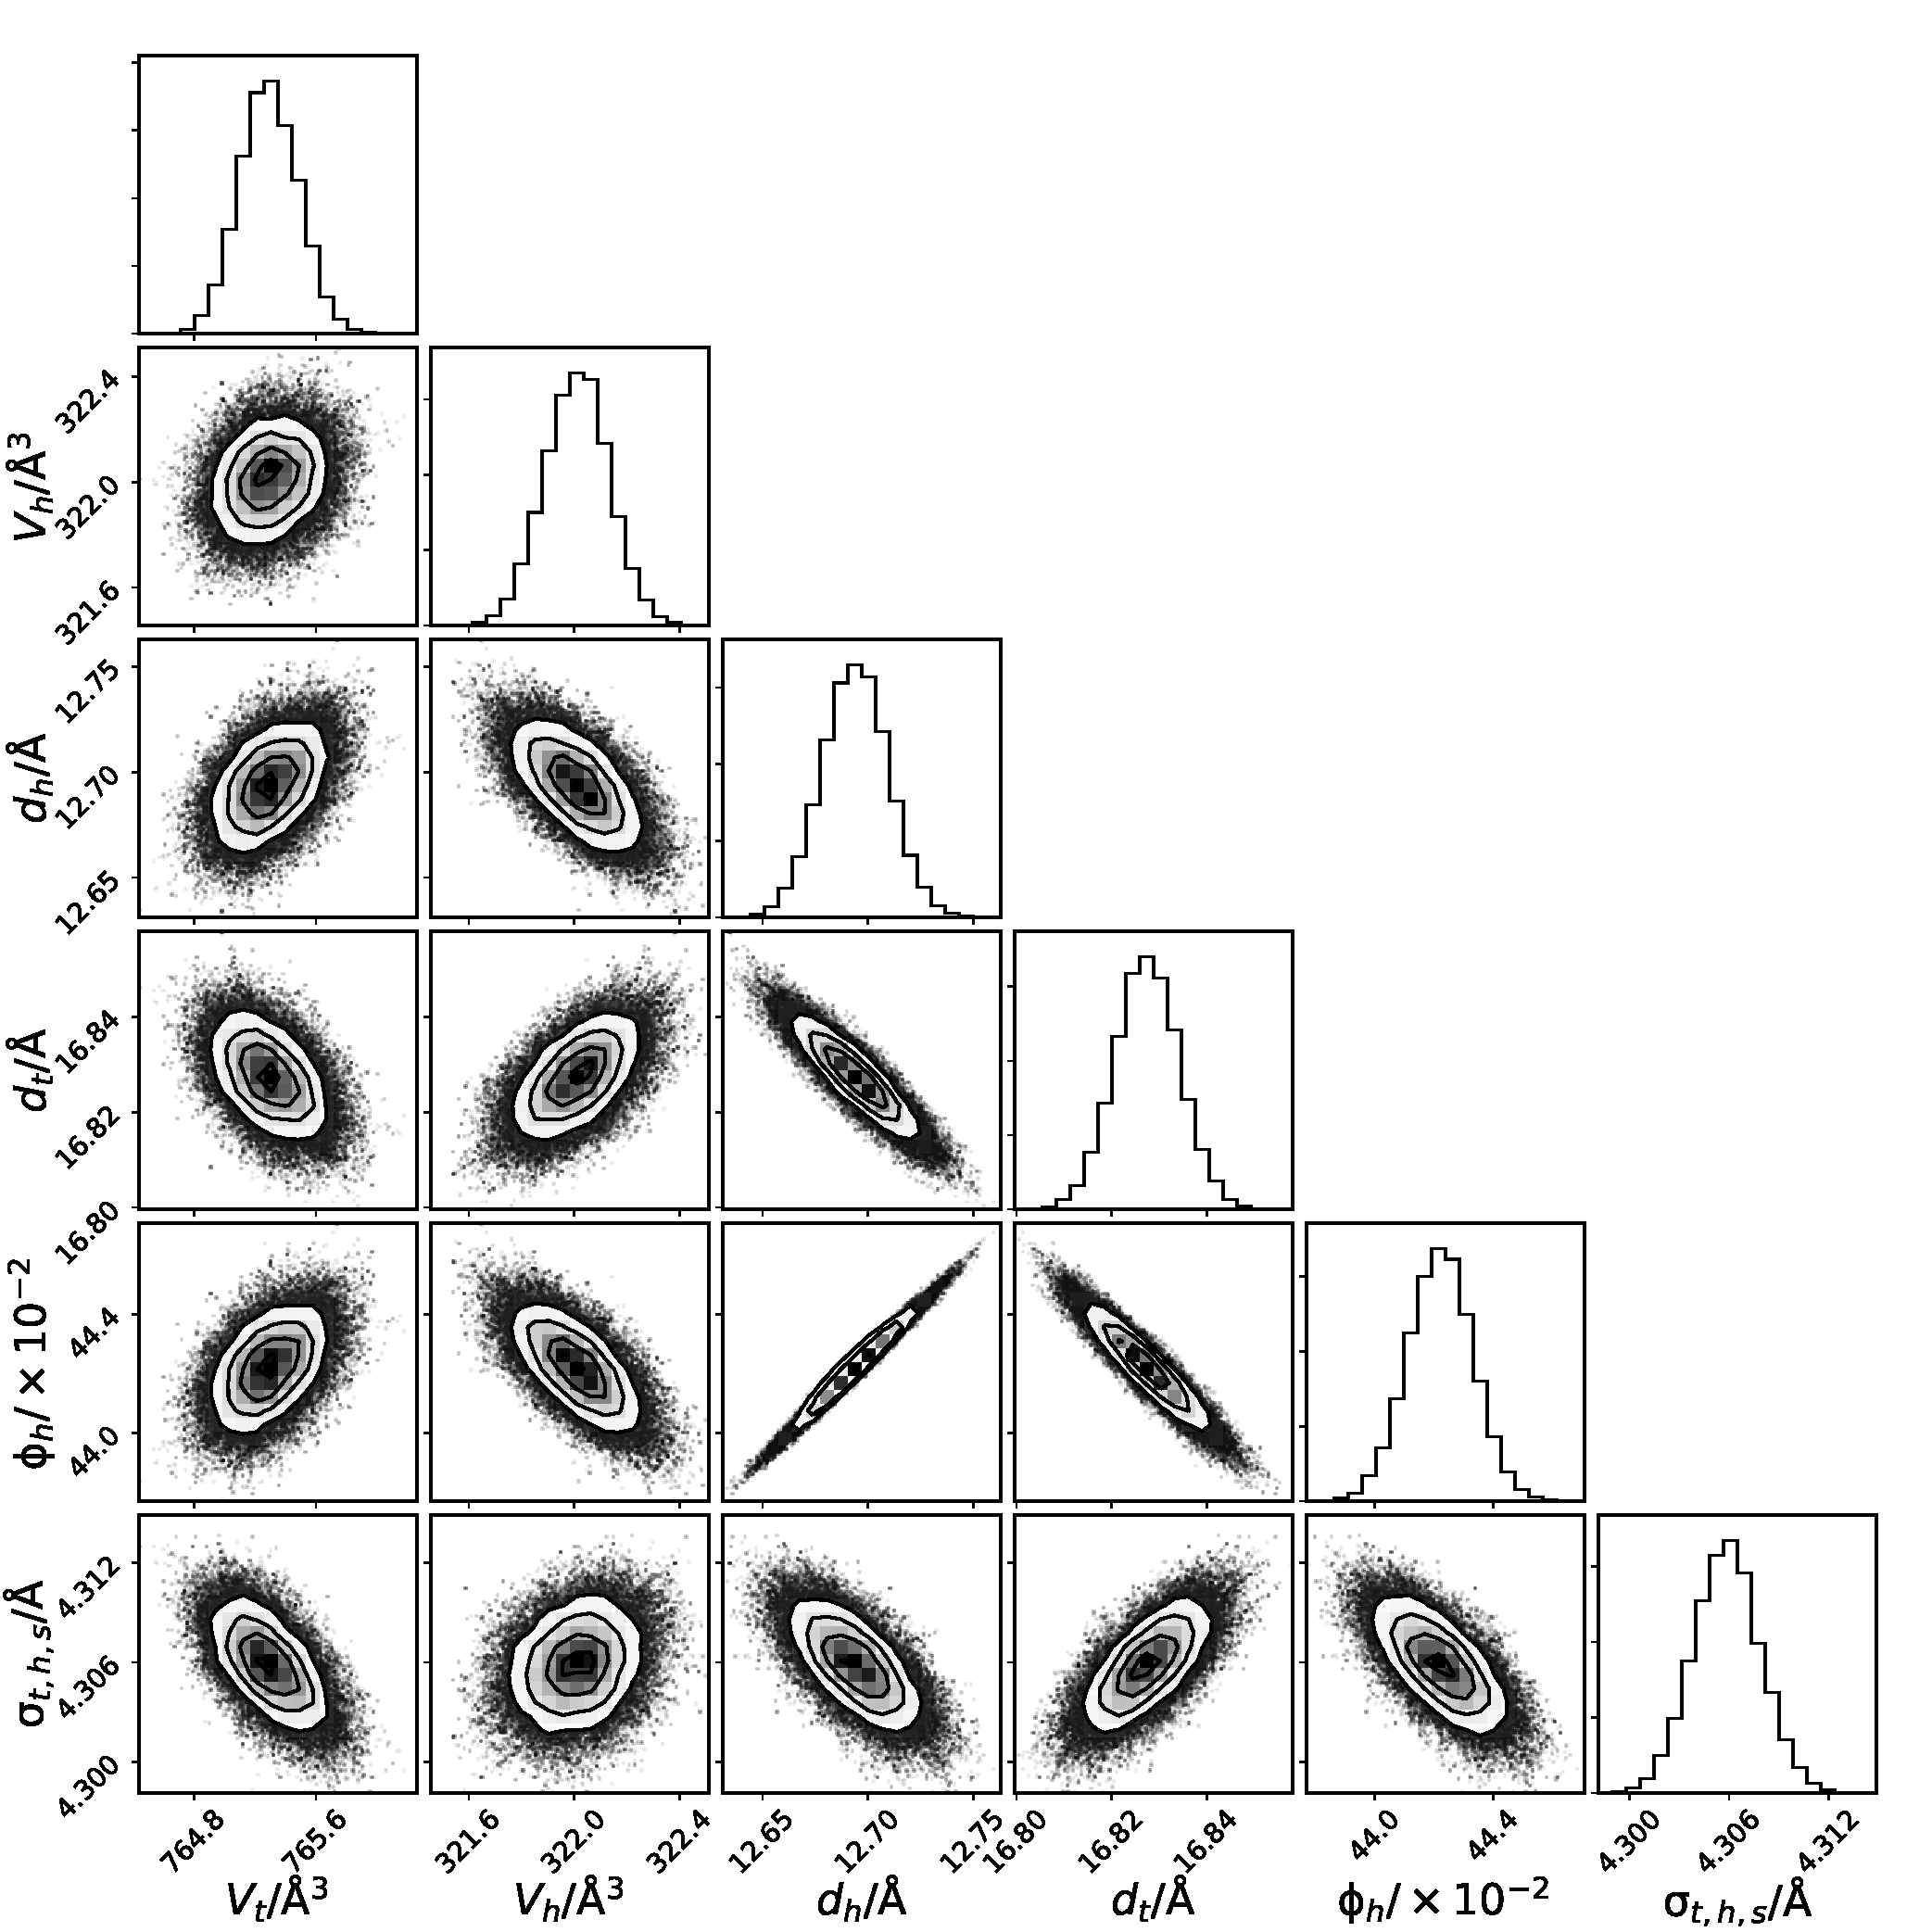
\includegraphics[width=0.50\textwidth]{figures/dppc3_all_corner}
	\caption{The multi-parameter PDFs for the chemically-consistent model of DPPC X-ray reflectometry data at \SI{25}{\milli\newton\per\meter}.}
	\label{fig:dppc3}
\end{figure}
\begin{figure}[H]
	\centering
	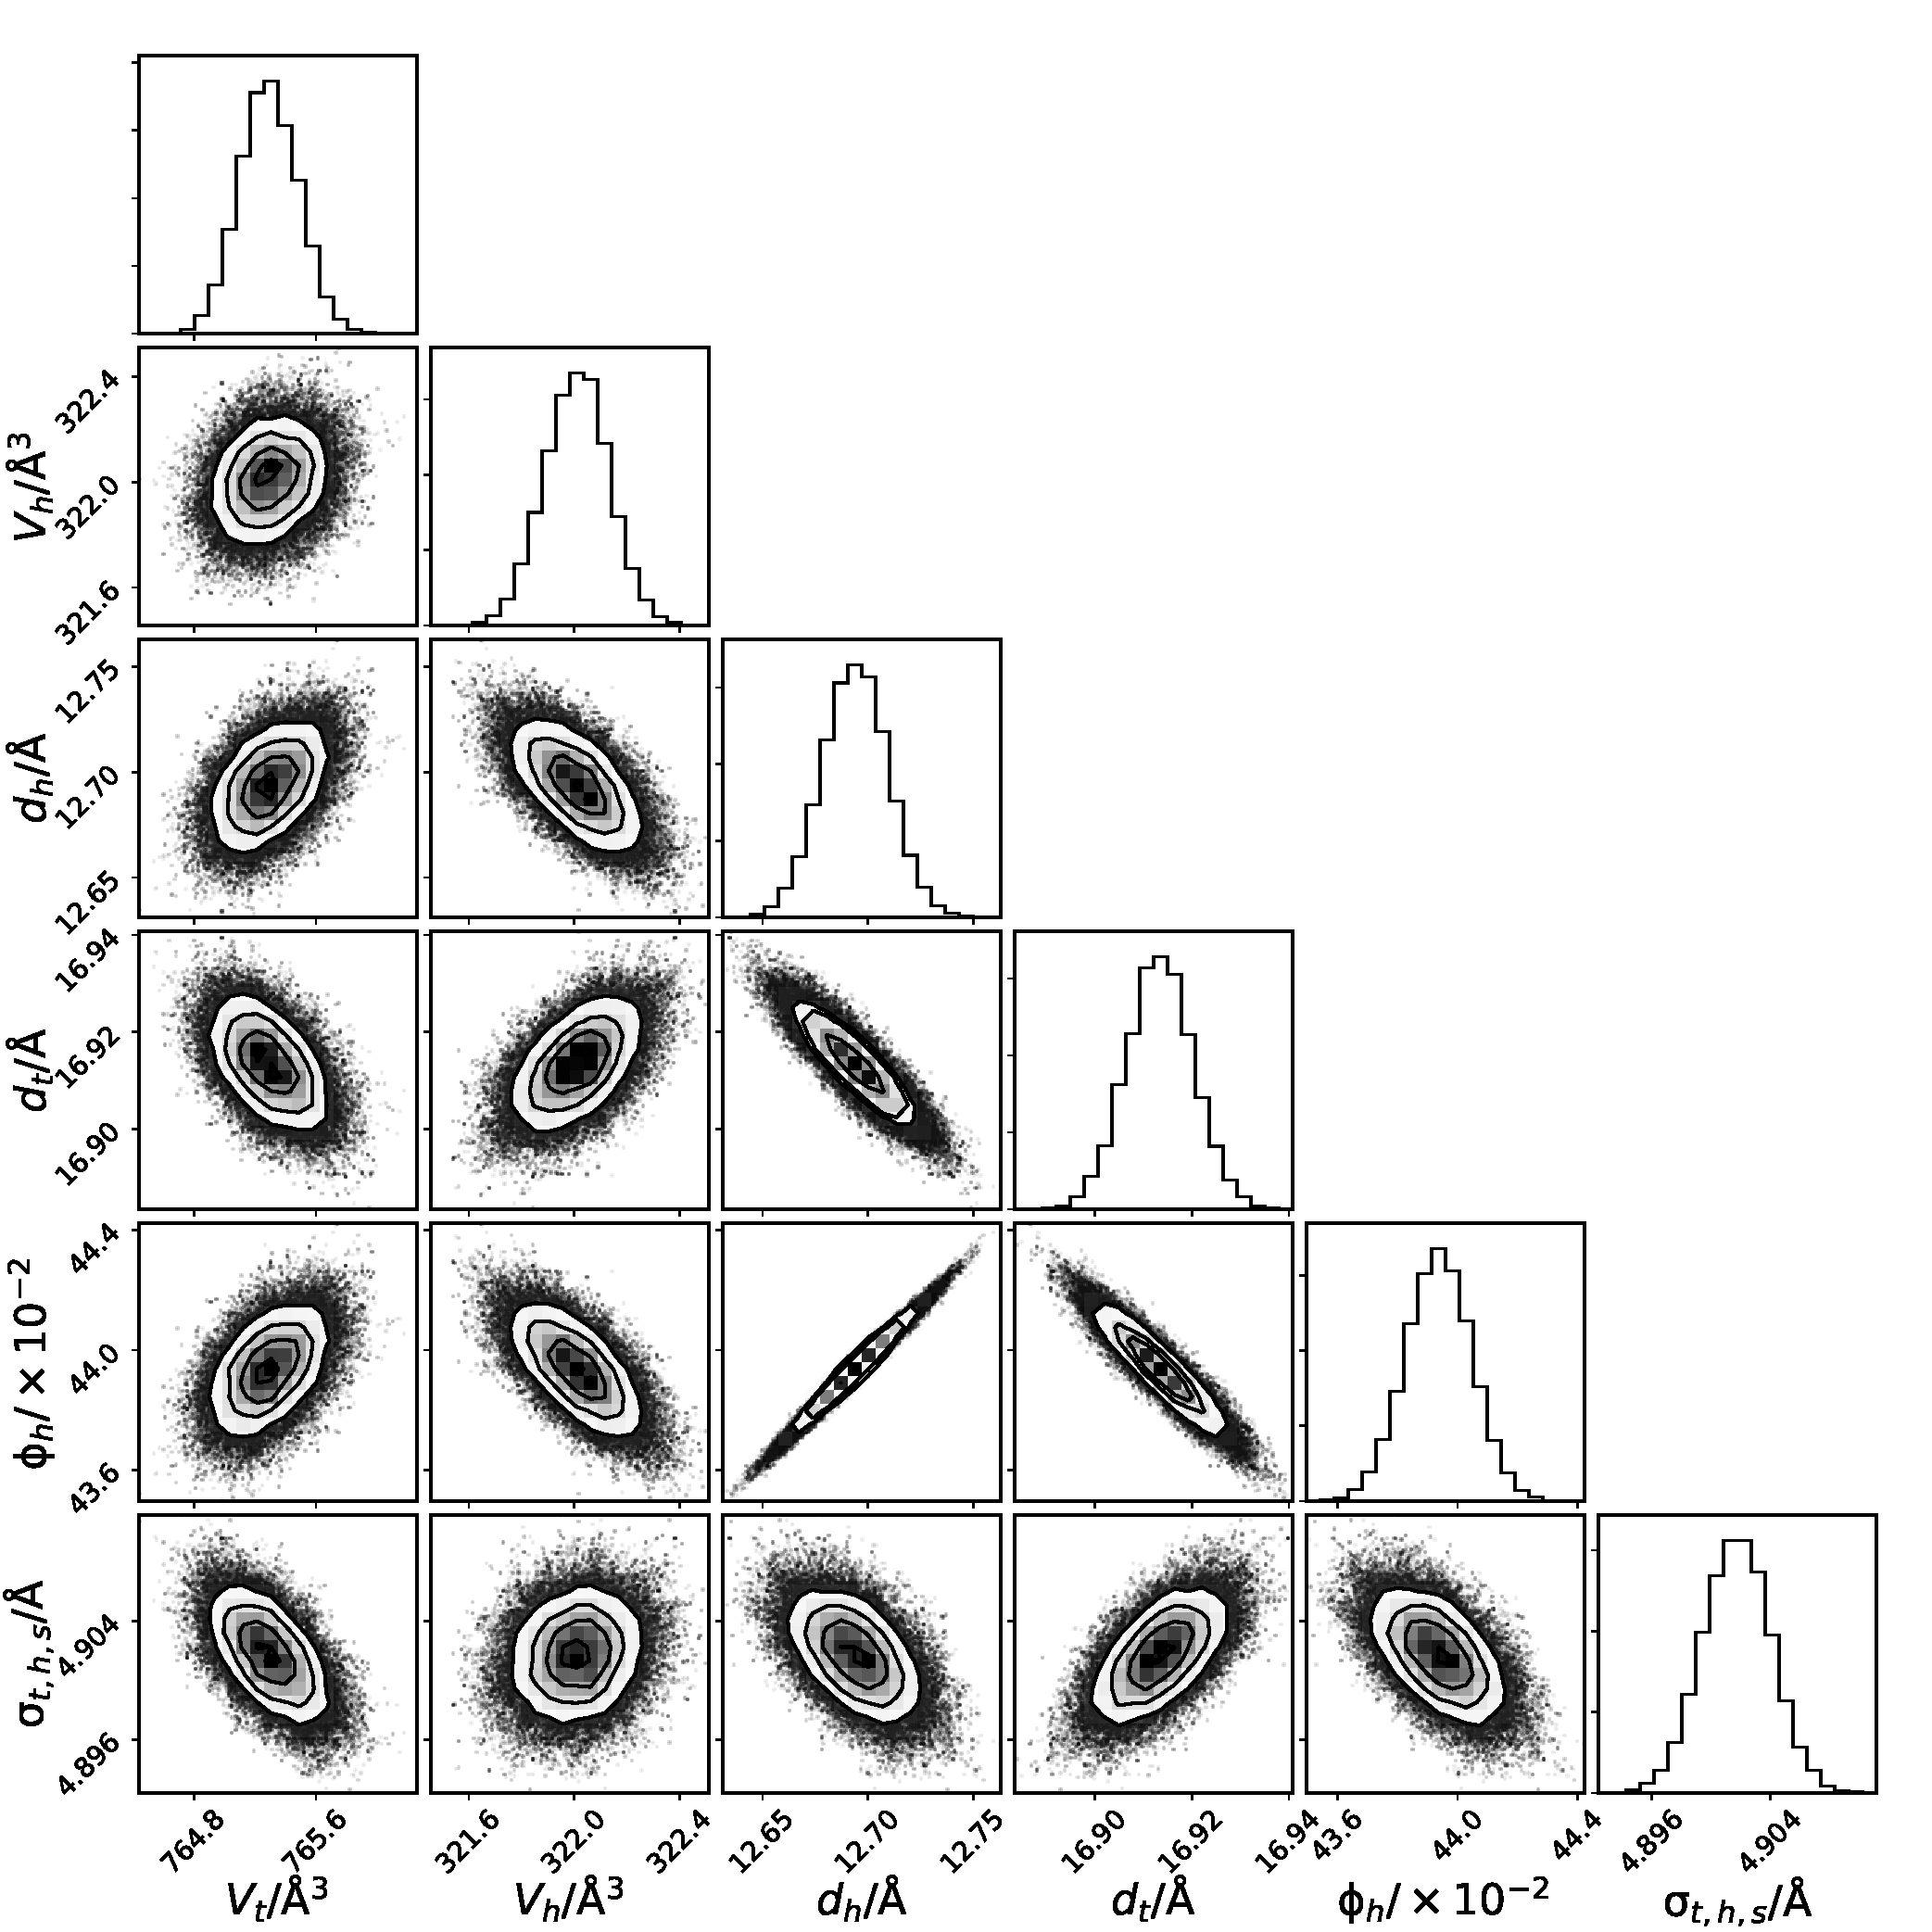
\includegraphics[width=0.50\textwidth]{figures/dppc4_all_corner}
	\caption{The multi-parameter PDFs for the chemically-consistent model of DPPC X-ray reflectometry data at \SI{30}{\milli\newton\per\meter}.}
	\label{fig:dppc4}
\end{figure}
\begin{figure}[H]
	\centering
	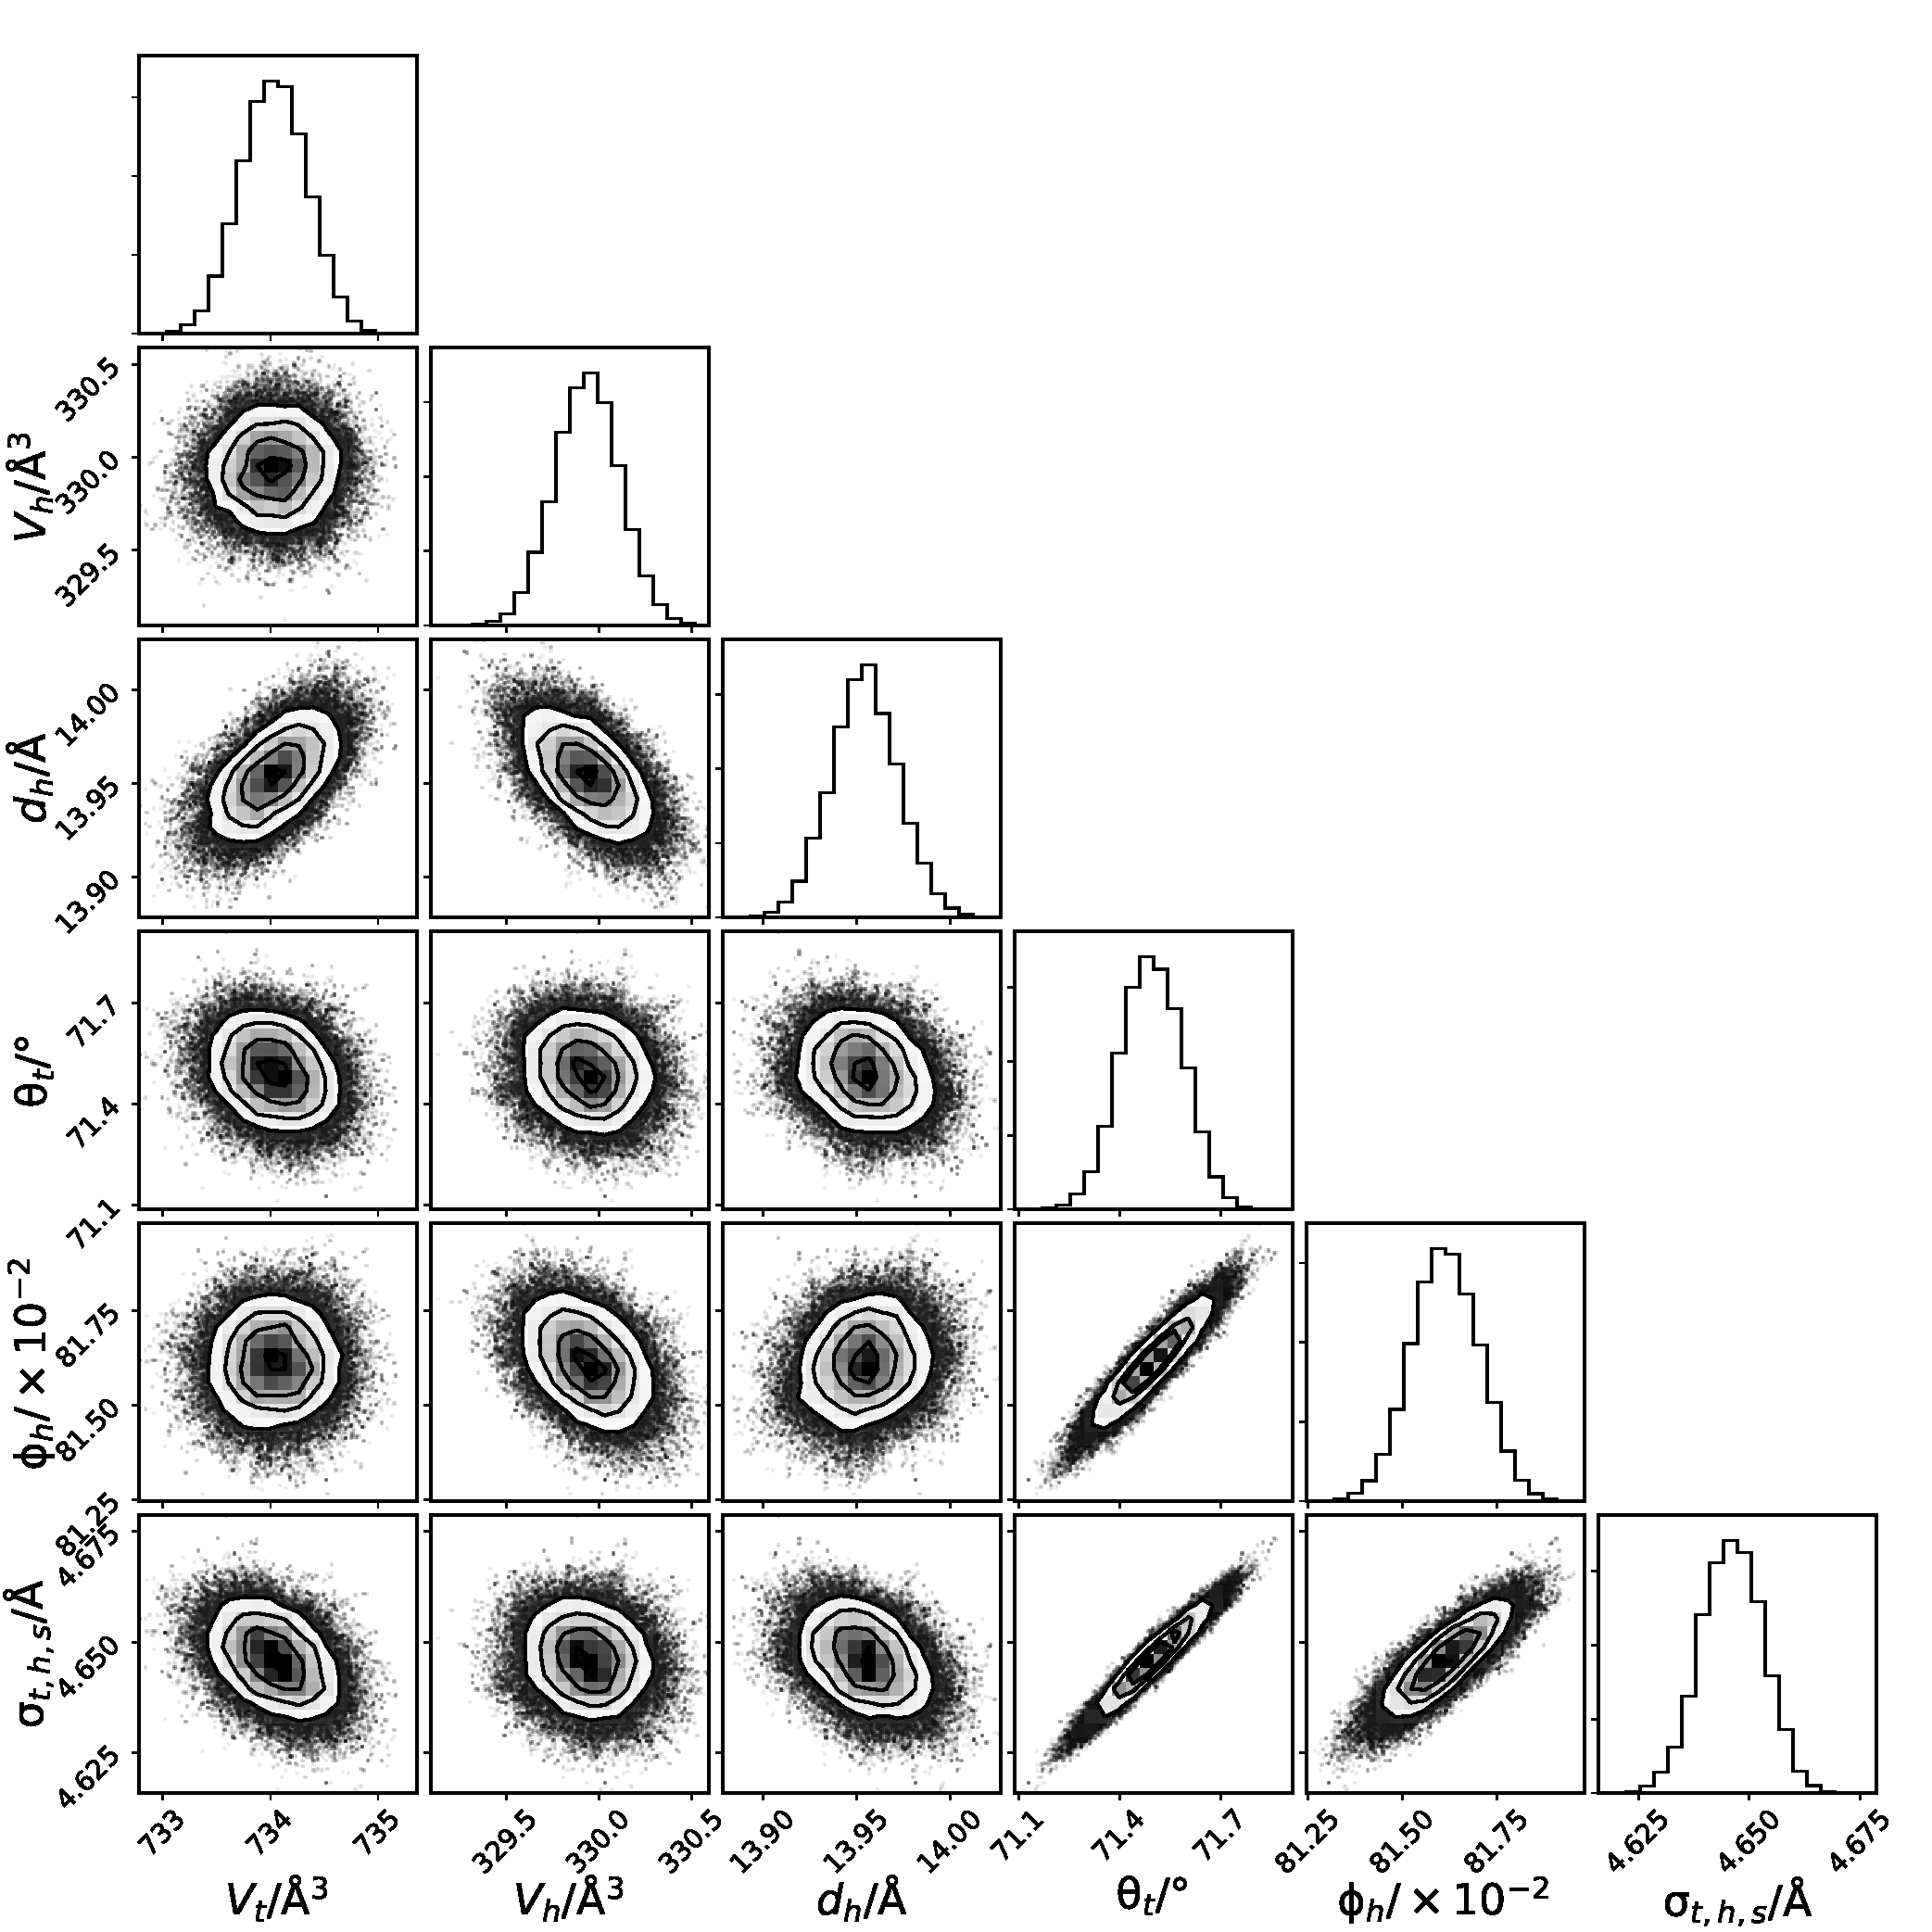
\includegraphics[width=0.50\textwidth]{figures/dmpg1_all_corner}
	\caption{The multi-parameter PDFs for the chemically-consistent model of DMPG X-ray reflectometry data at \SI{15}{\milli\newton\per\meter}.}
	\label{fig:dmpg1}
\end{figure}
\begin{figure}[H]
	\centering
	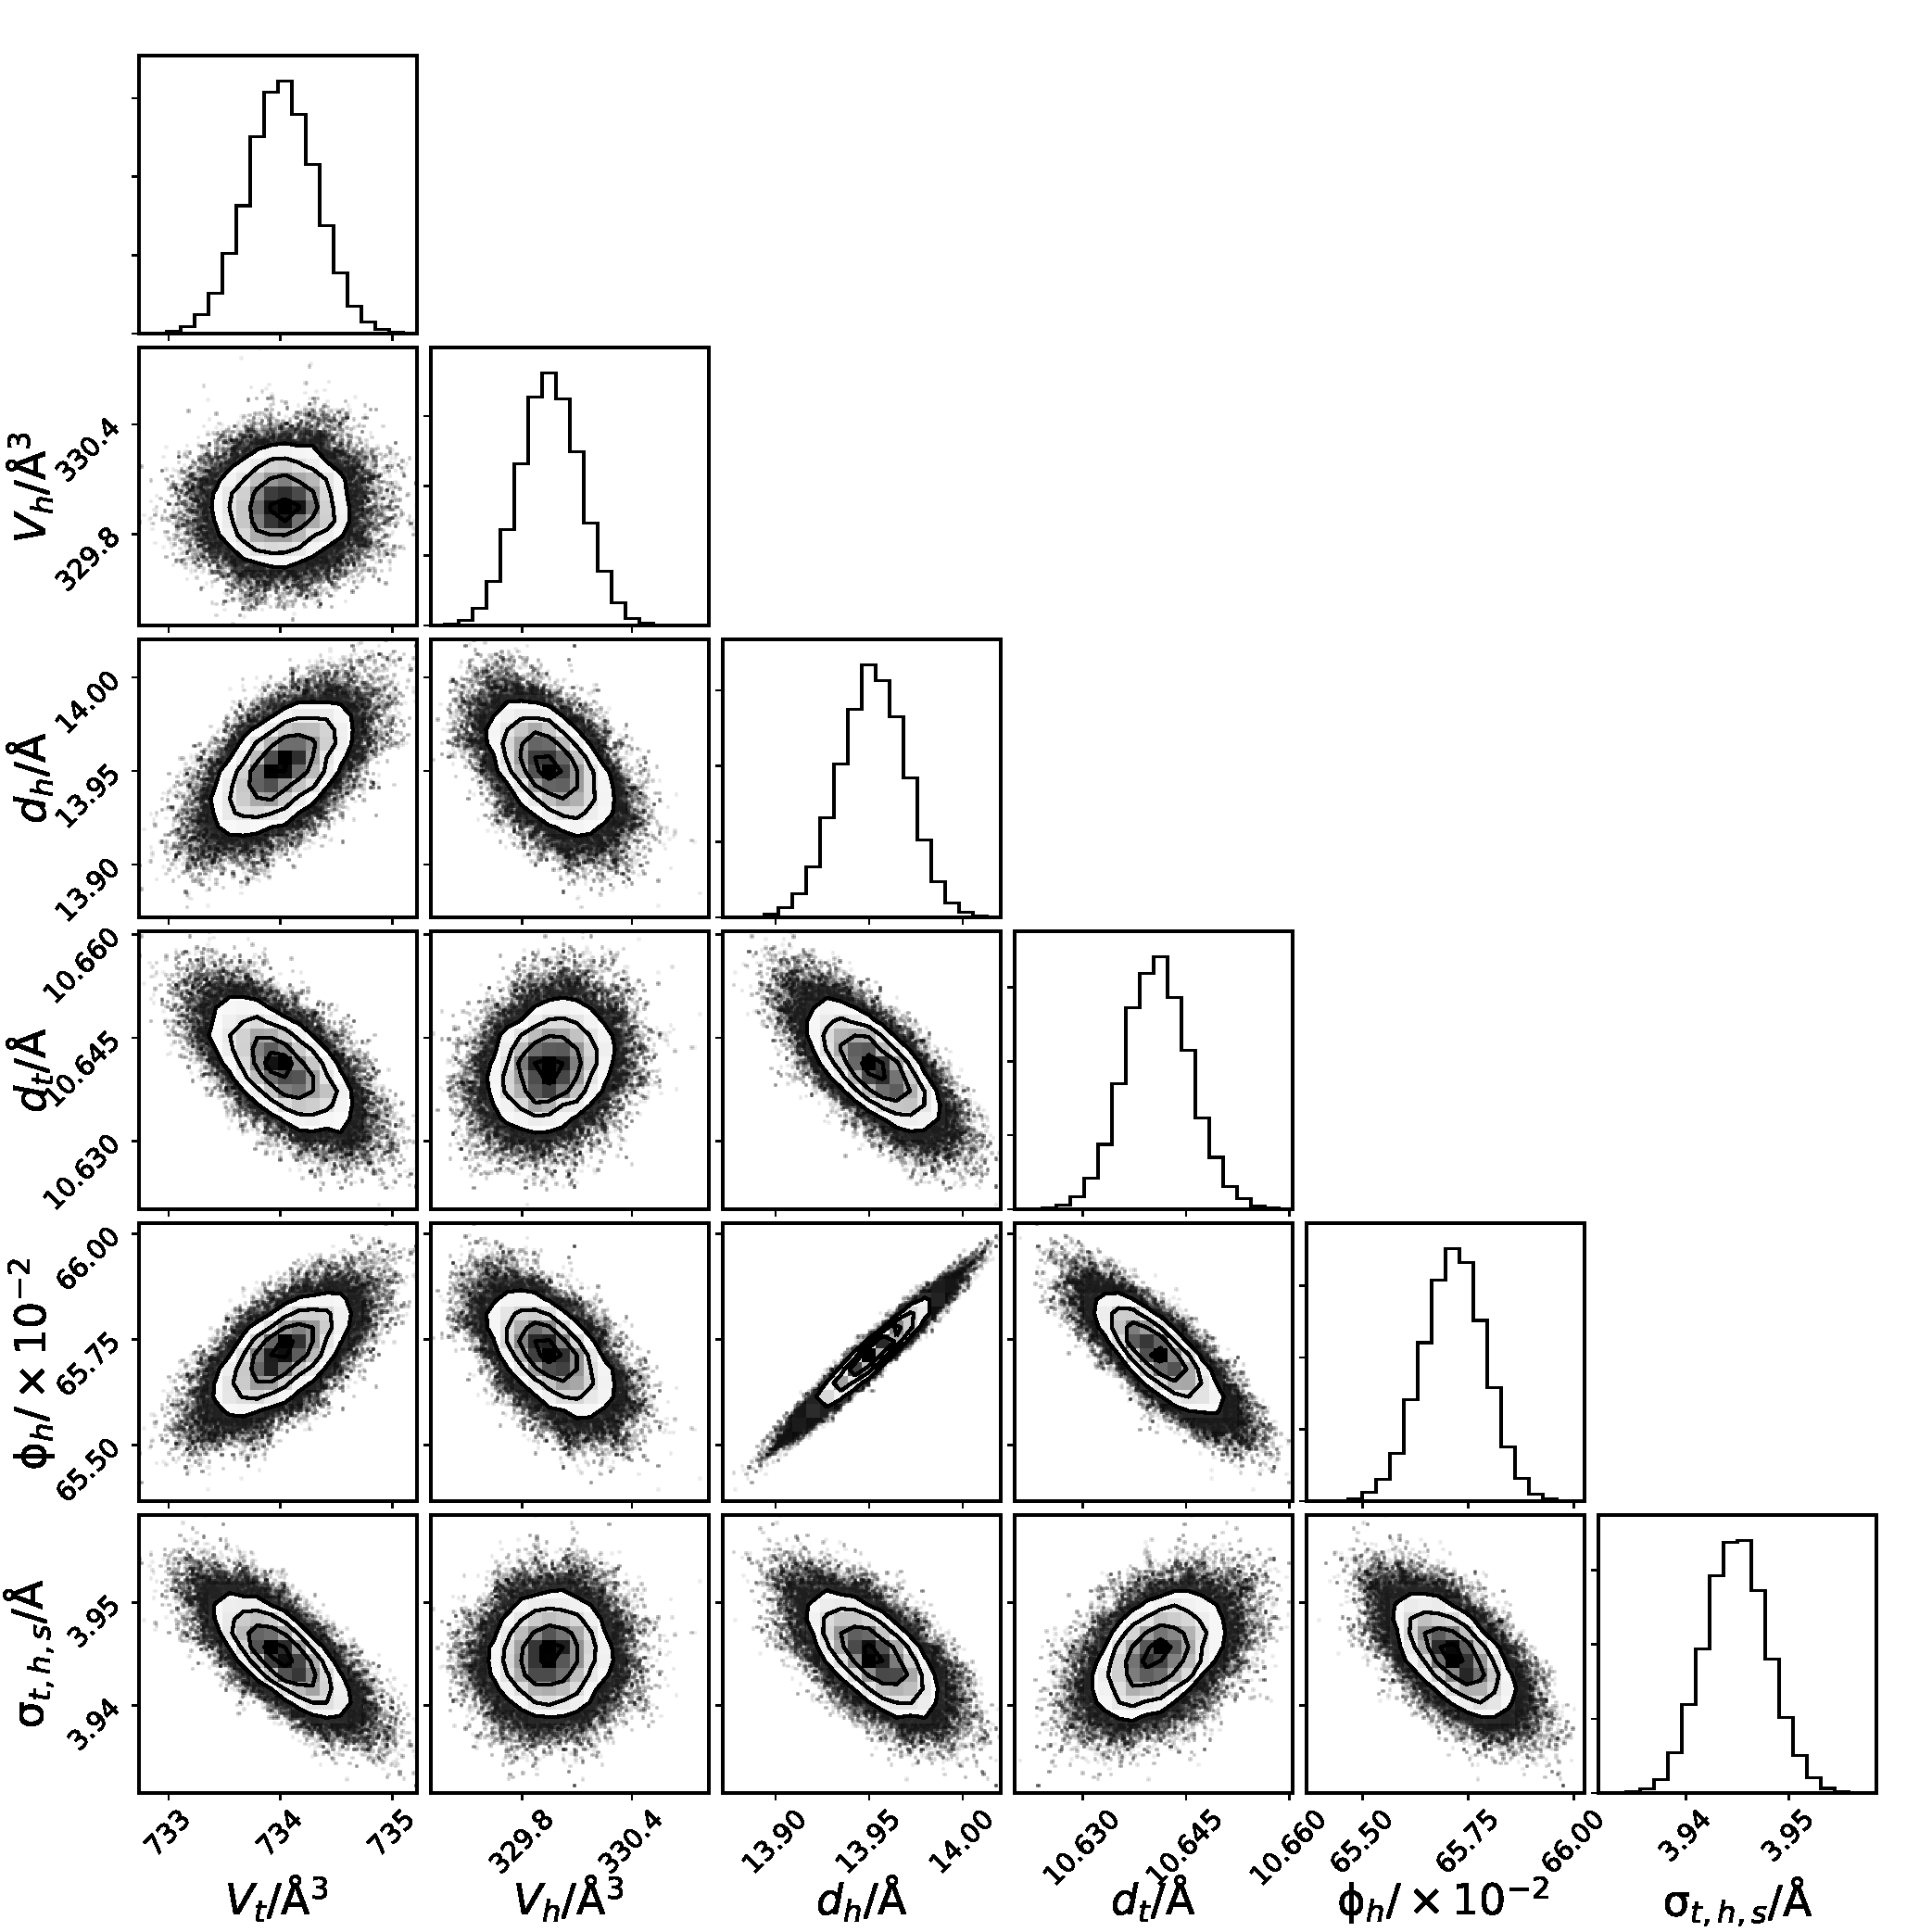
\includegraphics[width=0.50\textwidth]{figures/dmpg2_all_corner}
	\caption{The multi-parameter PDFs for the chemically-consistent model of DMPG X-ray reflectometry data at \SI{20}{\milli\newton\per\meter}. }
	\label{fig:dmpg2}
\end{figure}
\begin{figure}[H]
	\centering
	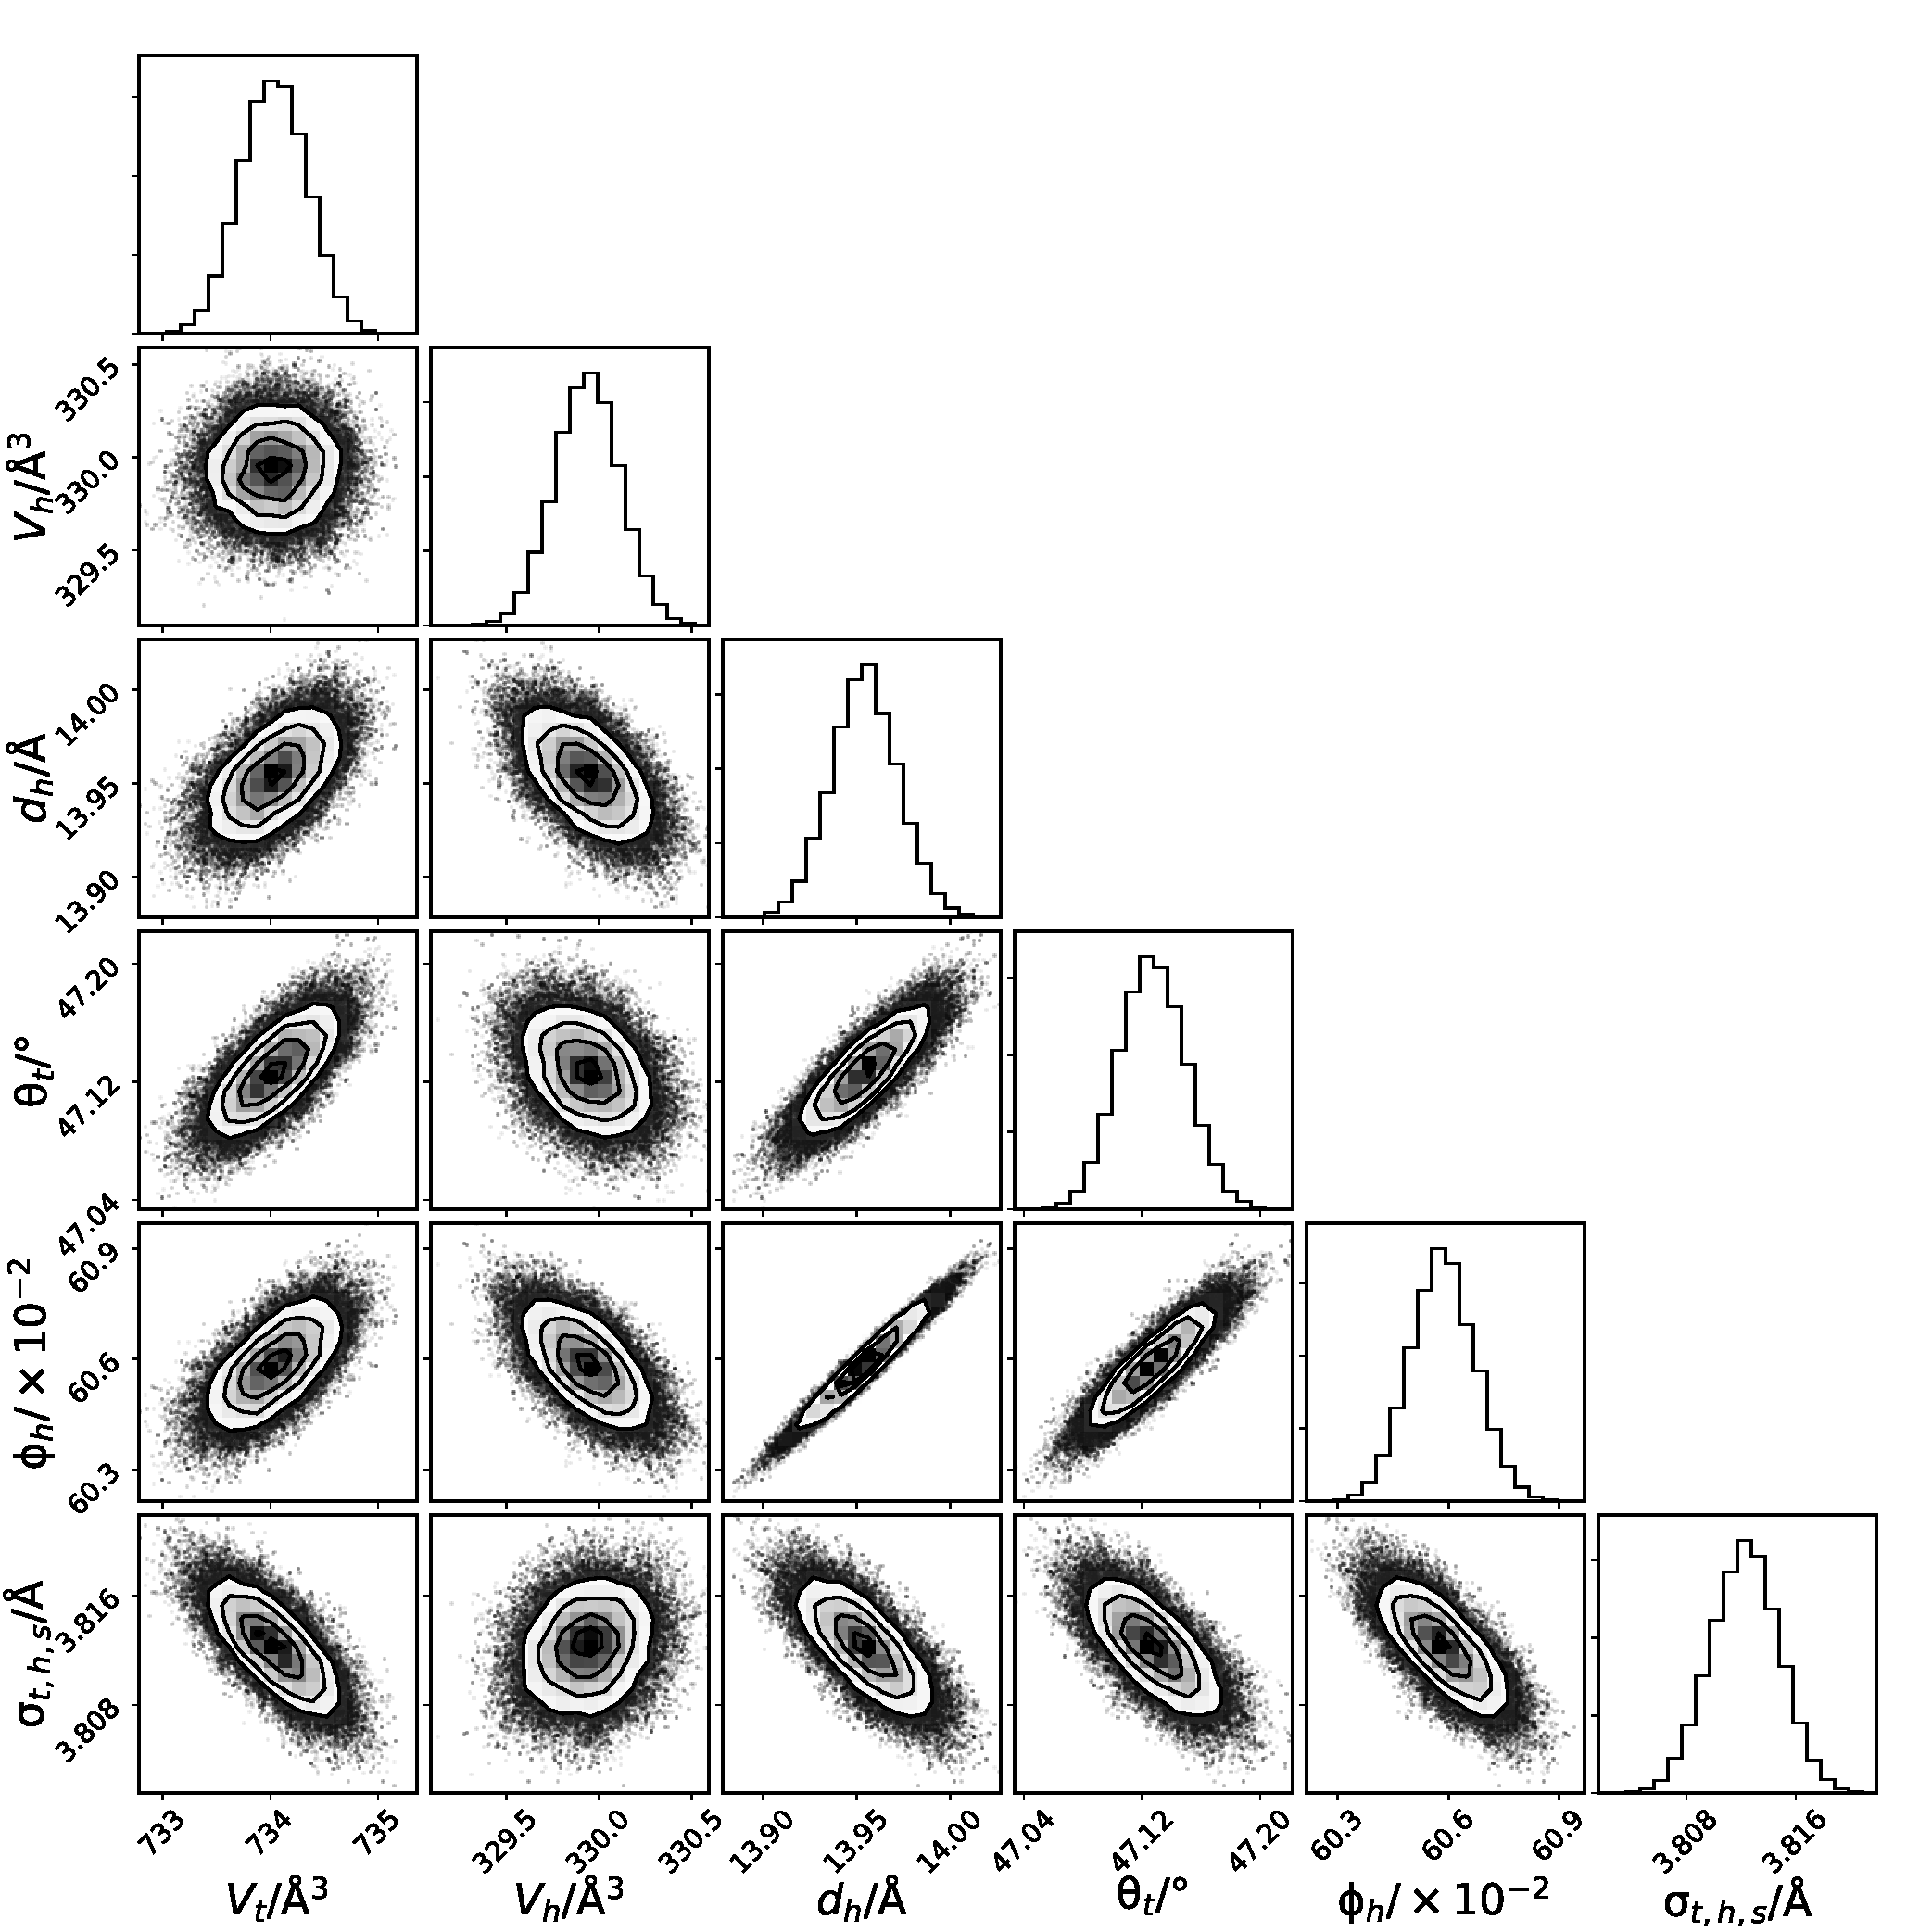
\includegraphics[width=0.50\textwidth]{figures/dmpg3_all_corner}
	\caption{The multi-parameter PDFs for the chemically-consistent model of DMPG X-ray reflectometry data at \SI{25}{\milli\newton\per\meter}.}
	\label{fig:dmpg3}
\end{figure}
\begin{figure}[H]
	\centering
	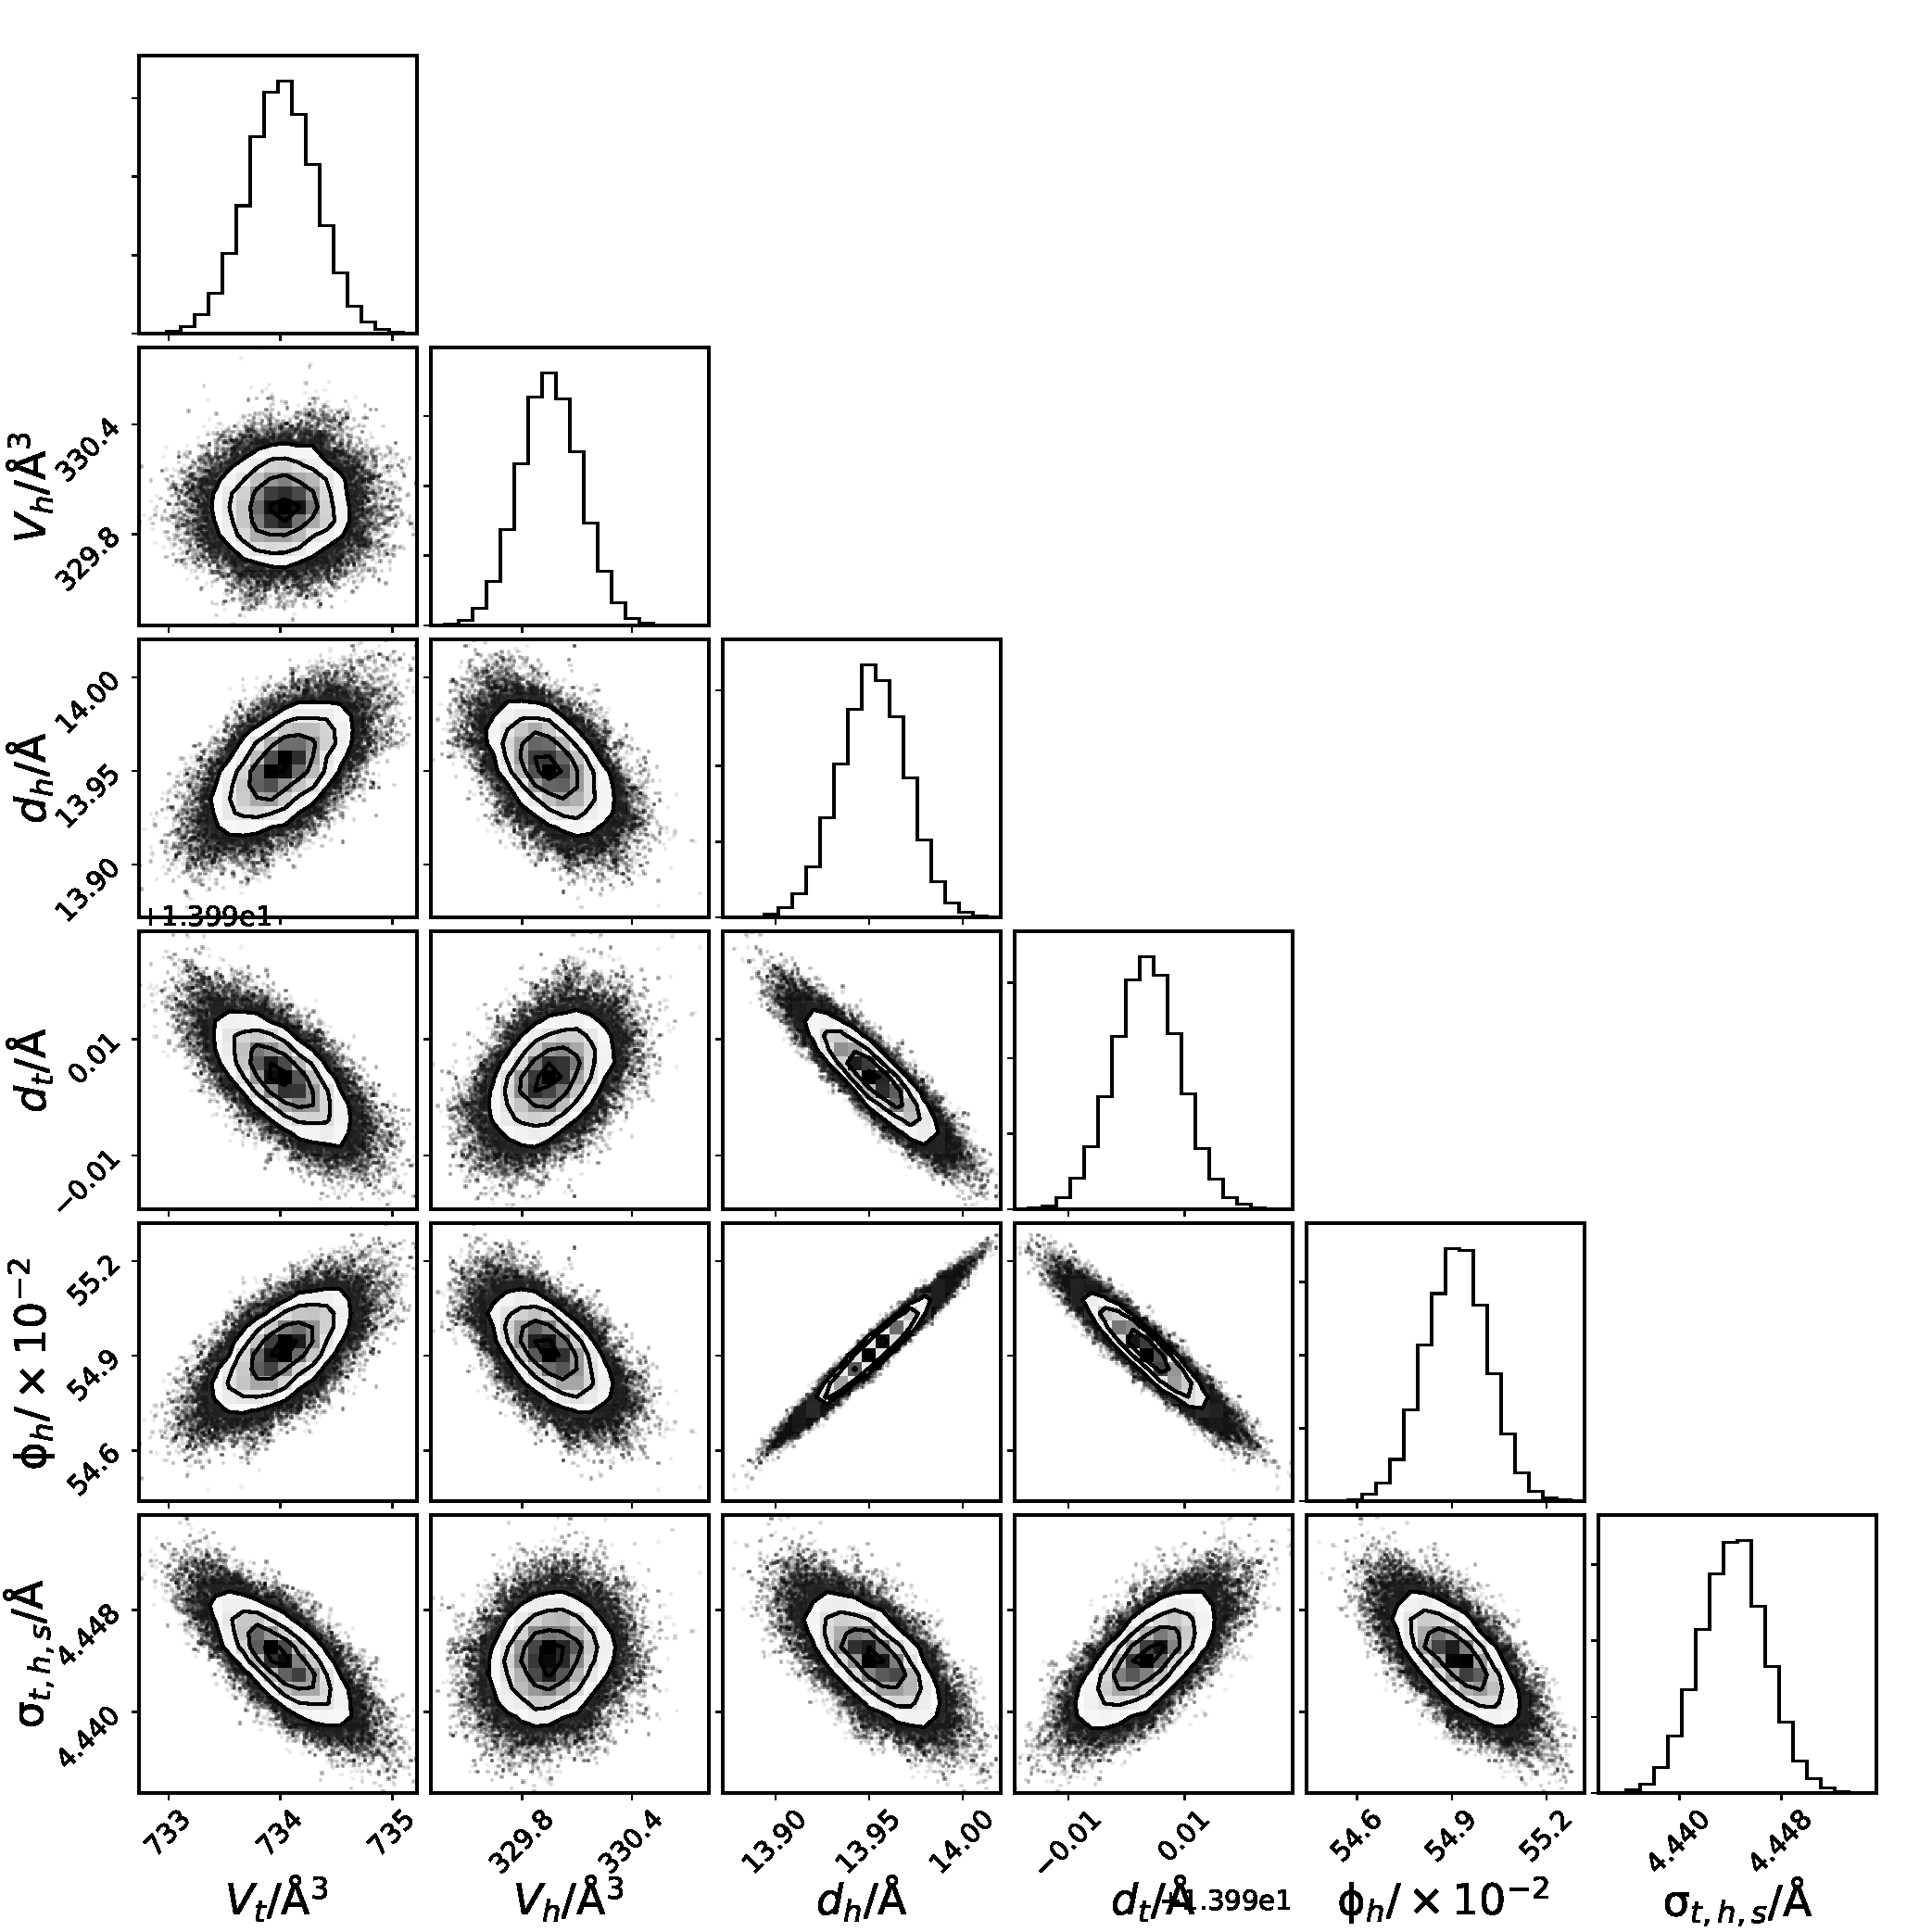
\includegraphics[width=0.50\textwidth]{figures/dmpg4_all_corner}
	\caption{The multi-parameter PDFs for the chemically-consistent model of DMPG X-ray reflectometry data at \SI{30}{\milli\newton\per\meter}.}
	\label{fig:dmpg4}
\end{figure}
\begin{figure}[H]
	\centering
	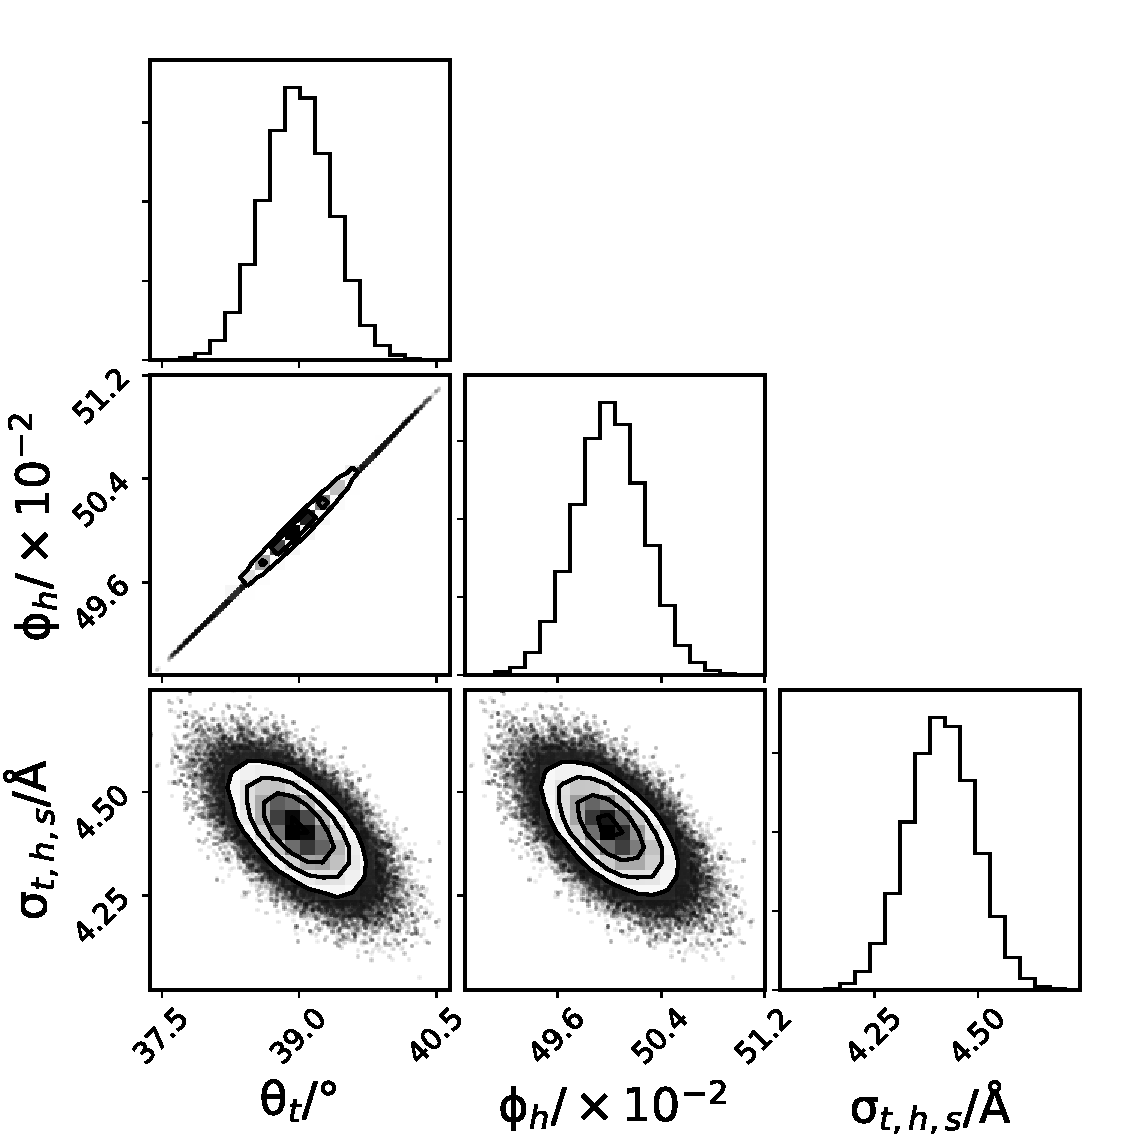
\includegraphics[width=0.50\textwidth]{figures/dmpc_20n_all_corner}
	\caption{The multi-parameter PDFs for the chemically-consistent model of two contrast DMPC neutron reflectometry data at \SI{20}{\milli\newton\per\meter}.}
	\label{fig:dmpcn1}
\end{figure}
\begin{figure}[H]
	\centering
	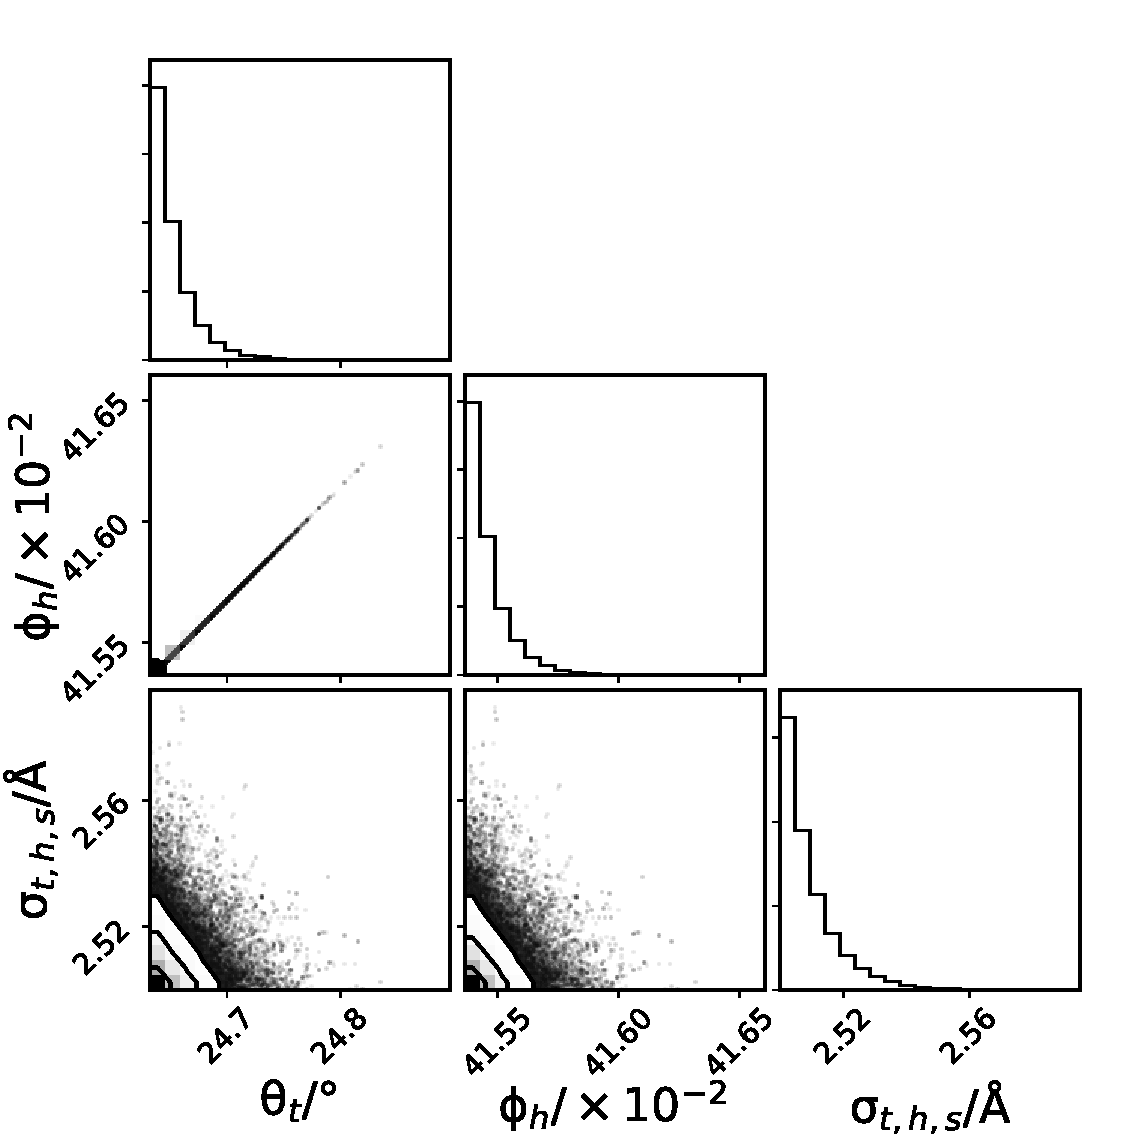
\includegraphics[width=0.50\textwidth]{figures/dmpc_25n_all_corner}
	\caption{The multi-parameter PDFs for the chemically-consistent model of two contrast DMPC neutron reflectometry data at \SI{25}{\milli\newton\per\meter}.}
	\label{fig:dmpcn2}
\end{figure}
\begin{figure}[H]
	\centering
	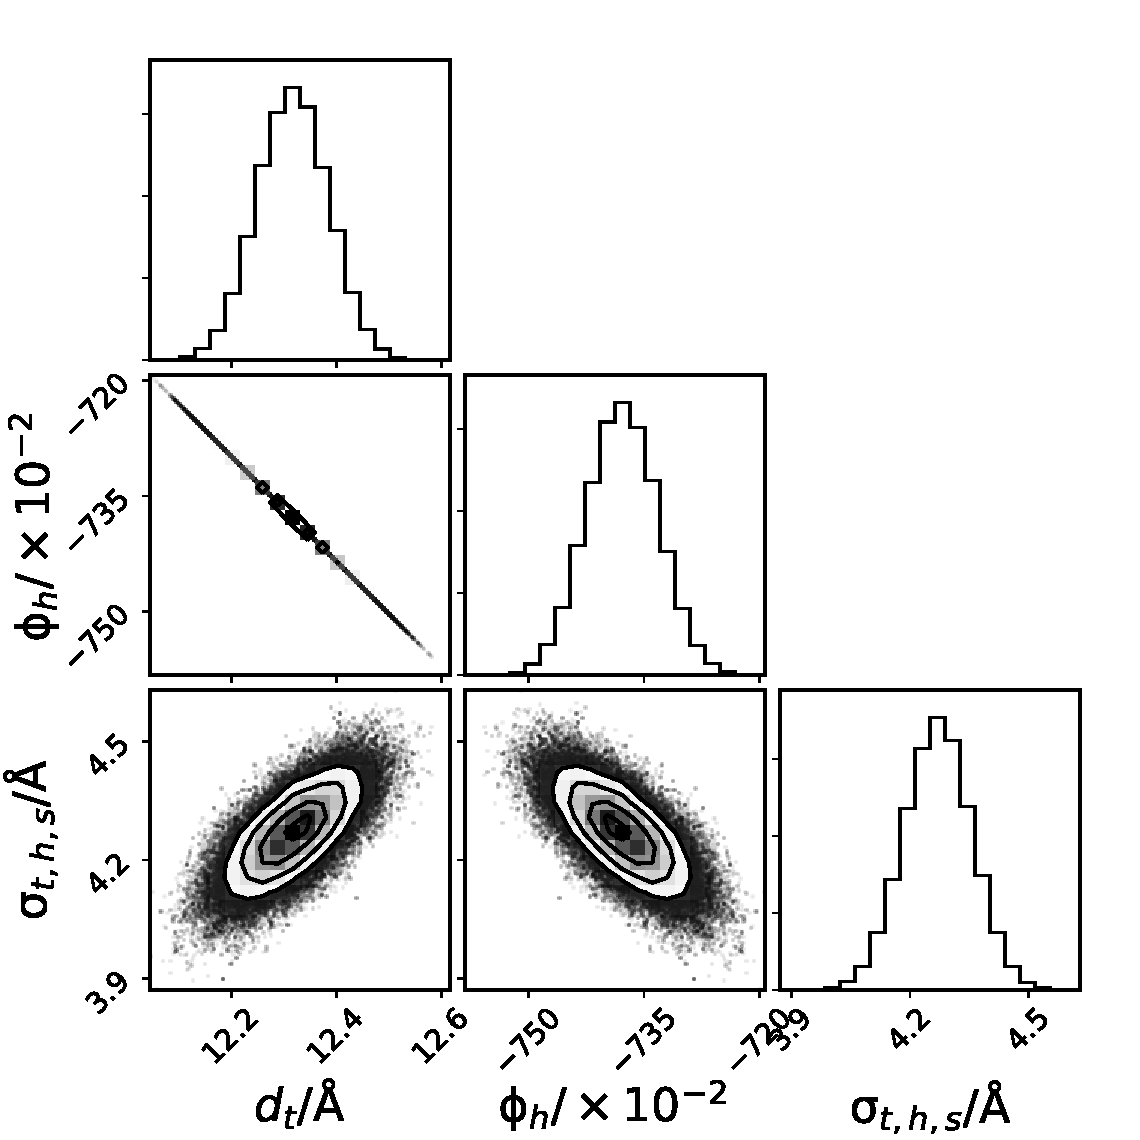
\includegraphics[width=0.50\textwidth]{figures/dppc_15n_all_corner}
	\caption{The multi-parameter PDFs for the chemically-consistent model of two contrast DPPC neutron reflectometry data at \SI{15}{\milli\newton\per\meter}.}
	\label{fig:dppcn1}
\end{figure}
\begin{figure}[H]
	\centering
	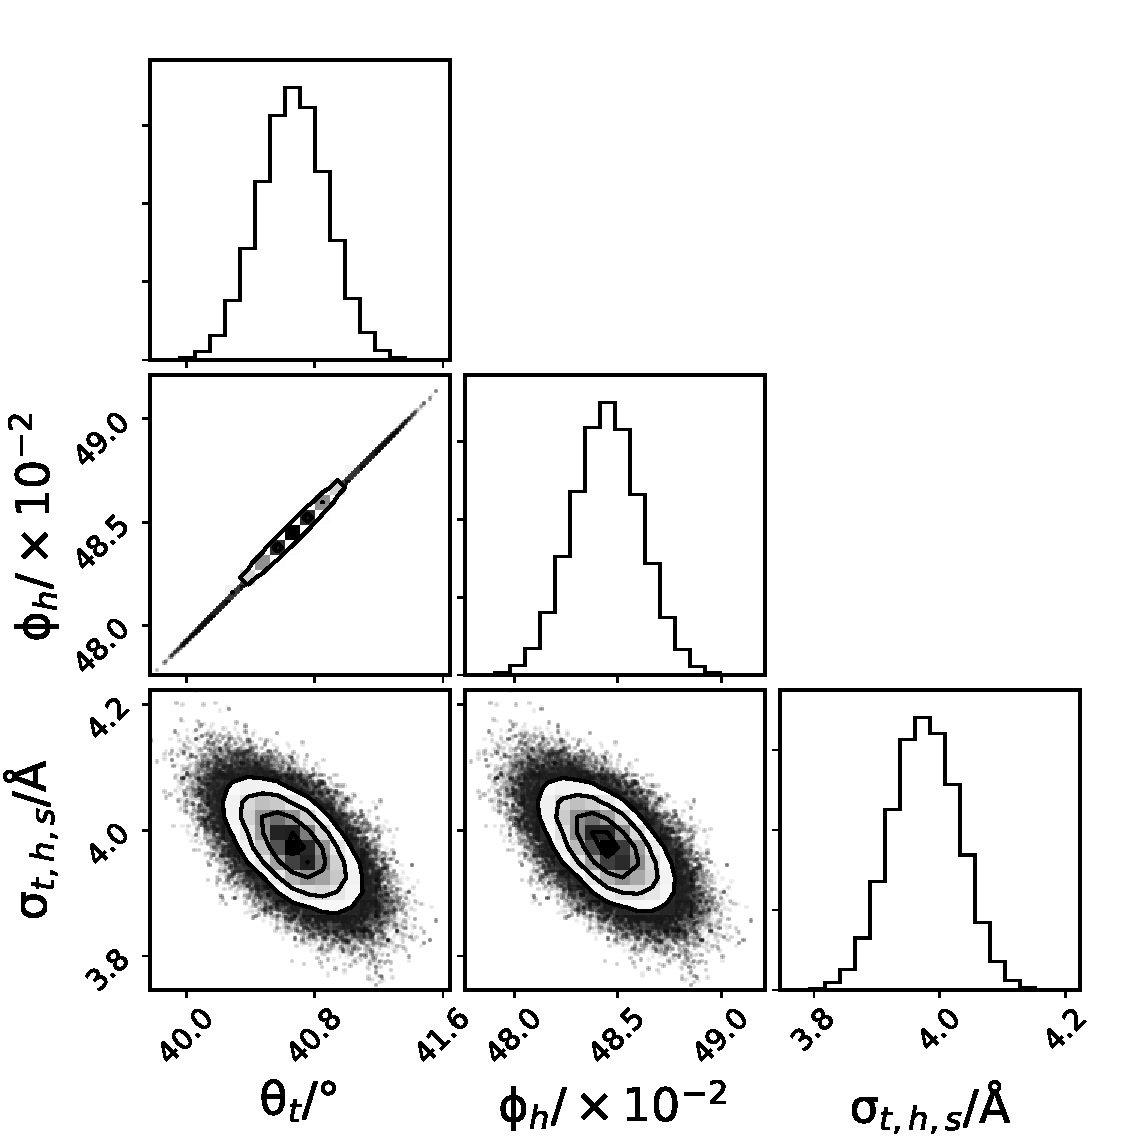
\includegraphics[width=0.50\textwidth]{figures/dppc_20n_all_corner}
	\caption{The multi-parameter PDFs for the chemically-consistent model of two contrast DMPC neutron reflectometry data at \SI{20}{\milli\newton\per\meter}.}
	\label{fig:dppcn2}
\end{figure}

%%%REFERENCES%%%
\bibliography{bibi} %You need to replace "rsc" on this line with the name of your .bib file
\bibliographystyle{rsc} %the RSC's .bst file
\end{document}
